% Documento principale

\documentstyle[amsfonts,../styles/psfig,../styles/tesisty,../styles/appsty]{../styles/deithesi}

% hyptesi.tex: contiene scomposizione in sillabe delle parole 
% Lista hyphenation.

\hy{a-do-zio-ne}
\hy{al-go-rit-mi}
\hy{a-ni-so-tro-po}
\hy{a-per-tu-ra}
\hy{bi-na-riz-za-zi-o-ne}
\hy{ca-rat-te-riz-za}
\hy{ca-mpio-na-men-to}
\hy{chi-u-su-ra}
\hy{co-lo-re}
\hy{co-me}
\hy{com-pat-ta}
\hy{con-si-de-ran-do}
\hy{con-si-de-ra-re}
\hy{con-si-de-ra-ta}
\hy{cor-ri-spon-de-reb-be}
\hy{co-stru-i-re}
\hy{de-ci-ma-zio-ne}
\hy{de-fi-ni-ti}
\hy{de-fi-ni-zi-o-ne}
\hy{de-fi-ni-ta}
\hy{del-l}
\hy{di-la-ta-zi-o-ne}
\hy{di-pen-do-no}
\hy{di-scri-mi-nan-te}
\hy{di-stri-bu-zi-o-ne}
\hy{do-mi-nan-te}
\hy{ec-ces-si-va}
\hy{ef-fi-ci-en-za}
\hy{e-ner-gi-a}
\hy{e-ro-sio-ne}
\hy{e-spri-mer-li}
\hy{e-ster-ne}
\hy{fi-gu-ra}
\hy{fi-ne-stra}
\hy{im-ma-gi-ne}
\hy{im-ma-gi-ni}
\hy{in-di-pen-den-te-men-te}
\hy{i-nol-tre}
\hy{in-ter-ne}
\hy{li-mi-ta-re}
\hy{li-ne-a-ri}
\hy{lo-ca-li}
\hy{lo-ca-liz-za-zi-o-ne}
\hy{ne-ces-sa-ri-a-men-te}
\hy{o-pe-ra-to-re}
\hy{o-pe-ra-to-ri}
\hy{o-pe-ra-zio-ne}
\hy{op-por-tu-ne}
\hy{or-di-na-men-to}
\hy{pic-co-le}
\hy{pos-si-bi-le}
\hy{pre-e-la-bo-ra-zi-o-ne}
\hy{pri-mi-ti-ve}
\hy{pro-ble-mi}
\hy{rap-pre-sen-ta-zio-ne}
\hy{ri-chi-e-de-re}
\hy{se-con-do}
\hy{se-gu-en-ti}
\hy{sod-di-sfa-no}
\hy{strut-tu-ra-le}
\hy{stru-cturing}
\hy{suf-fi-ci-en-te-men-te}
\hy{tra-scu-ra-bi-le}
\hy{tra-sla-zio-ni}
\hy{va-lo-ri}
\hy{va-ri-an-ze}
\hy{vo-le-va}

\includeonly{tesi-abstract,tesi-intro,tesi-operators,tesi-segment,tesi-bsplines,tesi-activecont,tesi-algor,tesi-final,tesi-append1,tesi-append2}

\begin{document}

%===================================================================================
% Indice generale
\tableofcontents

%===================================================================================
% Indice delle figure
\listoffigures

%===================================================================================
% Sommario (=Abstract)
% Sommario
\preface

%--------------------------------------------------------------------------------------------
In questa tesi ci si pone l'obiettivo di fornire una soluzione al problema della segmentazione
di macchie cutanee, i nei, per effettuare successivamente delle misure che possono riguardare
lo stato dei bordi, la forma e le simmetrie.

Il problema della segmentazione \e risolto utilizzando un algoritmo basato su un nuovo modello
di contorni attivi, {\it snakes} o {\it active contours}, in cui la funzione energia
potenziale, o funzione costo, non \e legata alla definizione del bordo come gradiente di una
immagine intensit\aac, ma \e funzione della distanza fra le intensit\a interna ed esterna
alla curva chiusa che individua lo snake.
Si realizza cos\iac\,\,la fusione delle informazioni locali nell'intorno dello snake e quelle
globali date dalla media delle intensit\aac\,\,nelle due regioni individuate.

Per quanto riguarda il modello del contorno si \e considerata la sua rappresentazione a
B-splines cubiche uniformi, la quale permette di mantenere la curva sufficientemente regolare
con una sua descrizione sufficientemente compatta; infatti essa \e descritta interamente da
un insieme limitato di parametri: i suoi {\it control points}.
Per permettere alla curva di adattarsi alla complessit\a dell'oggetto da segmentare, che per
sua natura non \e nota a priori, \e necessario rendere flessibile il numero dei control points;
\e stato perci\o definito un metodo di ridistribuzione dei campioni della curva con l'ausilio
di un reticolo, che rappresenta una scomposizione simpliciale (triangolazione) del piano
immagine.
L'associazione tra i nuovi campioni e i nuovi control points \e realizzata in base ad un
opportuno criterio che misura la complessit\a locale della curva nei punti campione
individuati.

Per migliorare le prestazioni della segmentazione \e opportuno partire da un contorno
iniziale prossimo a quello reale della macchia considerata, intendendo quindi tale
procedimento come una fase di presegmentazione.
Lo stato iniziale dello snake pu\o essere dato dal contorno della regione ottenuta a partire
dalla binarizzazione della componente principale della {\it trasformata di Karhunen-Lo\`eve}
(o di {Hotelling}) dell'immagine originale, successivamente elaborata con degli operatori
morfologici in modo che risulti compatta.

Elaborando la componente principale con un operatore locale anisotropo, il cui
comportamento in un punto dell'immagine dipende dalle caratteristiche dei punti in un
opportuno intorno, \e possibile definire una procedura per ridurre l'effetto di disturbo
di elementi come i peli.

%===================================================================================
% Introduzione
% Introduzione
\chapter{Introduzione}
%---------------------------------------------------------------------------------------------
Uno dei problemi posti in dermatoscopia \e la misura delle caratteristiche delle macchie
cutanee, per cui \e di interesse sviluppare degli strumenti che permettano di effettuare
tali misure in modo automatico.

Le misure riguardano generalmente le dimensioni, lo stato del bordo, se \e pi\u o meno
frastagliato, e le simmetrie sia relativamente alla forma sia rispetto alla pigmentazione
della superficie del neo.

Per poter effettuare tali misure \e necessario, per prima cosa, individuare la macchia, o neo,
estraendola dal contesto determinato dalla pelle circostante, tenendo presente gli elementi di
disturbo tipo i peli, le cui dimensioni non possono essere considerate sempre trascurabili
relativamente a quelle del neo.

\vs(5)

Due sono quindi gli obiettivi che ci si \e proposti di raggiungere:
\ben
\im un problema di {\it segmentazione}: individuare il neo;
\im rappresentazione semplice e compatta del suo contorno per facilitare le successive misure.
\een

Per quanto riguarda la segmentazione esiste un'ampia scelta di metodi che si sviluppano a
partire da due modi equivalenti di interpretare il problema.
I primi definiscono la soluzione come la partizione dell'immagine in regioni uniformi, ovvero
la partizione a cardinalit\a massima ottenibile rispetto ad un dato criterio di uniformit\aac,
che nel nostro caso potrebbe essere il colore (in quanto il neo \e una regione con
pigmentazione differente, generalmente pi\u scura, rispetto alla pelle circostante).
La seconda classe di metodi invece considera come obiettivo l'individuazione dei contorni che
separano le diverse regioni.

Concettualmente le due tecniche sono equivalenti, in pratica, hanno un comportamento
complementare: nel primo caso si ha una minor sensibilit\a al rumore presente
nell'intorno dei contorni mentre si ha difficilmente una rappresentazione compatta dei
segmenti ottenuti; nel secondo caso invece si ha una maggior sensibilit\a al rumore,
ma al contrario si ha una maggior capacit\a di localizzazione dei bordi \e la possibilit\a
di ottenere rappresentazioni compatte del contorno dei segmenti, in particolare con l'utilizzo
di opportuni modelli di {\it contorni attivi} ({\it active contours} o {\it snakes}) che sono
trattati in questa tesi.

Recentemente sono stati proposti inoltre degli algoritmi con combinano i due
approcci (\cite{Duncan}, \cite{Yuille} e \cite{Yezzi}) in modo da compensarne i difetti e
sommarne i vantaggi.
La prima soluzione \cite{Duncan} prevede l'interazione dei due blocchi distinti attraverso
una serie di regole che stabiliscono come i due interagiscono fino a raggiungere uno stato di
equilibrio.

La seconda soluzione, che \e qui considerata, realizza l'obiettivo a partire dalla
definizione di un nuovo modello di snakes in cui i contorni non sono direttamente
caratterizzati come le zone ad alto gradiente, ma indirettamente attraverso
una nuova funzione energia che tiene conto della statistica delle regioni separate dallo
snake e che \e minima quando questi si dispone lungo il contorno dell'oggetto considerato.
In particolare l'algoritmo proposto da Yezzi et al. in \cite{Yezzi} presenta delle specifiche
che lo rendono interessante per la semplicit\a della definizione della funzione energia e 
per ci\o che ne consegue in termini di implementazione.

L'algoritmo permette infatti di segmentare l'immagine nei suoi diversi elementi non appena
sia fissata la primitiva, {\it feature}, rispetto alla quale risultano distinti; \e da
notare che non \e necessario conoscere il valore della primitiva caratteristico di ciascun
oggetto ma \e sufficiente sapere che per ciascuno \e differente.
Un'altro vantaggio rilevante \e dato dal fatto che la definizione data permette di considerare
non una sola feature alla volta, ma contemporaneamente un vettore di features che possono
essere di natura diversa tra loro.
Nel caso specifico permette di trattare le immagini a colori che sono matrici $R \times C$ di 
pixels a ciascuno dei quali \e associato un vettore di tre elementi, nel caso pi\u semplice
le tre componenti $RGB$.

Accanto alla definizione della funzione energia occorre definire il modello che 
rappresenta fisicamente la curva chiusa e quindi lo snake: si \e scelta
una rappresentazione a B-splines cubiche uniformi.
La curva \e rappresentata perci\o come l'unione di tratti di cubica ({\it spans}) che sono
combinati secondo dei parametri, i punti di controllo o {\it control points}; l'ordine del
polinomio definisce il grado di regolarit\a della curva.

In tal modo si \e ottenuta una rappresentazione compatta, come si voleva, 
interamente rappresentata dai punti di controllo, che sono in numero limitato, e rispetto
ai quali \e possibile definire le misure delle caratteristiche geometriche del contorno.

Un problema associato alla scelta del metodo di segmentazione riguarda l'inizializzazione
del contorno attivo: lo snake definito in \cite{Yezzi} concettualmente \e 
abbastanza insensibile all'inizializzazione (in pratica vi possono essere dei limiti se
l'immagine non \e considerabile bimodale) a differenza dei modelli di snake precedenti che
si basano sulla ricerca degli edge nell'intorno della curva e per i quali \e opportuna una
buona inizializzazione.
In ogni caso \e opportuna per ridurre i tempi di esecuzione dell'algoritmo.

L'inizializzazione si pu\o intendere come una fase di presegmentazione ed \e data dal
contorno della regione ricavata binarizzando la componenete principale della
{\it trasformata di Karhunen-Lo\`eve} (o di {\it Hotelling}) dell'immagine originale, seguita
da alcune elaborazioni con operatori morfologici per ottenere una regione compatta.
Inizializzando la curva in prossimit\a del bordo della macchia \e possibile realizzare
un'implementazione locale dell'algoritmo di Yezzi che permette di ridurre le due regioni
interna ed esterna a due fascie definite nell'intorno dello snake.
In tal modo si ha che le due aree possono essere approssimativamente uguali, indipendentemente
dalle dimensioni della macchia rispetto al piano immagine, ed inoltre \e
possibile escludere le zone prossime ai bordi del sensore, maggiormente sensibili ai disturbi
dovuti alla illuminazione non uniforme e agli stessi effetti di bordo dell'ottica.

In questa fase \e possibile inoltre ridurre gli elementi di disturbo come i peli: 
sfruttando il fatto che questi hanno una elevata correlazione lungo una direzione, che
\e comunque incognita, \e possibile realizzare un operatore locale che
elabora l'immagine in funzione della misura di anisotropia rilevata nell'intorno
del punto considerato. 
Esistono diverse definizioni per tale misura, nel nostro caso si \e considerata una funzione
della media dei valori dell'intensit\a della stessa componente principale lungo
direzioni\footnotemark\, prefissate; quindi in corrispondenza dei punti che
si considerano appartenenti al pelo, per cui la misura \e superiore ad un valore di soglia,
si sostituisce il valore dell'intensit\a con un nuovo valore che dipende dai pixels
circostanti che molto probabilmente appartengono alla cute o al neo.

\footnotetext{Considerando che tali rette-direzioni sono definite in uno spazio non
 continuo ma discreto (segmenti di rette digitali).}

A partire dalla curva iniziale, definita da un certo numero di control points distribuiti
nel piano, \e necessario permettere che questa possa adattarsi alla complessit\a 
dell'oggetto che rileva durante la sua evoluzione.
Si \e pensato quindi di realizzare una riparametrizzazione della curva, basata su un
metodo di {\it triangolazione} (o {\it scomposizione simpliciale}), e la definizione
di un criterio di complessit\a per determinare un nuovo numero di punti di controllo.
 

%--------------------------------------------------------------------------------------------
% Contenuto dei capitoli
\contcap{Contenuto dei capitoli}

\begin{description}
\im[\sl Capitolo 2.] Sono descritti alcuni operatori per l'elaborazione digitale delle
   immagini:
   \bi
   	\im {\it trasformata di Karhunen-Lo\`eve}
   	\im {\it operatori morfologici}
   	\im {\it rank-order filters}
   \ei	
\im[\sl Capitolo 3.] Introduzione al problema della segmentazione e descrizione di alcuni
   algoritmi di binarizzazione.
\im[\sl Capitolo 4.] Definizione e propriet\a delle B-splines.
\im[\sl Capitolo 5.] I modelli dei contorni attivi: l'approccio statistico proposto da
   Yezzi et al. \cite{Yezzi}.
\im[\sl Capitolo 6.] Descrizione dell'architettura dell'algoritmo proposto con alcuni
   risultati.
\end{description}

\finepar
%===================================================================================
% Corpo della tesi

% Operatori per l'elaborazione digitale delle immagini
\chapter{Operatori per l'elaborazione digitale delle immagini}\lb{OEDI}

%======================================================================================
\section{Cambiamento di risoluzione}

Le immagini analogiche generate da un sistema ottico per poter essere memorizzate ed
elaborate vengono campionate nelle coordinate spaziali e quantizzate nell'intensit\a.
La suddivisione dell'immagine in $M$ righe e $N$ colonne individua un numero finito
$M \cdot N$ di elementi d'immagine ({\it pixel}); $M$ ed $N$ specificano quindi la risoluzione
dell'immagine.
In alcuni casi un'alta definizione pu\o risultare non indispensabile e anzi costituire
un limite all'efficienza dell'algoritmo in quanto si ha un elevata quantit\a di dati da
analizzare.
Inoltre vi sono applicazioni in cui si sfrutta la possibilit\a di analizzare l'immagine a
diverse scale di definizione per poter individuare alcune strutture dell'imma-gine che
risultano invarianti al variare della risoluzione.
In particolare con l'adozione di opportune strutture dati come la piramide di immagini 
(\cite{Zamperoni}, \cite{Meer}).

%-------------------------------------------------------------------------------------
\subsection{Riduzione della risoluzione}

La trasformazione che porta alla riduzione della risoluzione mappa necessariamente diversi
punti dell'immagine ad alta risoluzione in un punto di quella a risoluzione inferiore.
Il caso pi\u semplice \e dato dal campionamento in cui si considerano, ad esempio, i punti
dell'immagine ad indici dispari:

\vs(5)

sia $f\,(\,x\,,\,y\,)$ l'immagine di partenza di dimensioni $(\,R,C\,)$, con $R$ e $C$
pari, allora  
\be
h\,(\,x\,,\,y\,)\,=\,f\,(\,2\,x\,-\,1\,,\,2\,y\,-\,1\,)
\lb{campion}
\ee

con le due dimensione ridotta di un fattore $2$. 

\vs (5)

A causa della riduzione della risoluzione si pu\o avere una perdita nella definizione di 
alcuni dettagli dell'immagine; tale perdita di informazione che pu\o essere limitata
con un'opportuna scelta del nucleo della trasformazione stessa, per esempio considerando
la media del valore dei pixel nell'intorno del punto considerato\footnotemark:
\beqa
h\,(\,x\,,\,y\,) & = & \frac{1}{4}\,[\,f\,(\,2\,x\,-\,1\,,\,2\,y\,-\,1\,)\,+\, 
                                     f\,(\,2\,x\,-\,1\,,\,2\,y\,)\,+ \nonumber\\
                 &   &              +\,f\,(\,2\,x\,,\,2\,y\,-\,1\,)\,+\,
                                     f\,(\,2\,x\,,\,2\,y\,-\,1\,)\,]
\lb{media}
\eeqa
\footnotetext{La costruzione della piramide di immagini pu\o essere visto come un processo
di decimazione, per cui il nucleo che rende minima la perdita d'informazione dovuta al
campionamento, ovvero che permette la ricostruzione dell'immagine originale, \e il filtro
passa-basso ideale.}

Per un maggior approfondimento sulla scelta del nucleo si pu\o far riferimento a quanto
riportato in \cite{Meer}.

%======================================================================================
\section{Trasformazioni dello spazio dei colori}

Generalmente le immagini a colori sono rappresentate per mezzo del modello $RGB$, dove ad ogni
pixel \e associato un vettore tridimensionale le cui componenti sono proprio i valori
di rosso $R$, verde $G$ e blu $B$ in cui \e possibile scomporre il colore percepito del pixel.

Una rappresentazione di questo tipo \e per\o legata alle caratteristiche del sensore (CCD) che
ha fornito l'immagine per cui spesso si ricorre ad altri spazi in cui rappresentare le 
propriet\a intrinseche del colore meno sensibili alle 
caratteristiche del sensore stesso.

Esiste una vasta gamma di possibili modelli, trasformazioni, metriche che possono essere
utilizzate per evidenziare le propriet\a utili alle diverse applicazioni \cite{Wyszecki}; nel nostro
caso si sono considerate la trasformazione che permette di ottenere le componenti $HSI$
del colore e la {\it trasformazione di Karhunen-Lo\`eve}.

%-------------------------------------------------------------------------------------
\subsection{Lo spazio HSI}

La trasformazione che mappa lo spazio $RGB$ nello spazio $HSI$ (o $HSV$) \e non lineare con
alcune singolarit\a:
\bi

\im (\,{\it Hue}\,) {\it Tonalit\a}: caratterizza il colore dominante nel punto {\bf x} 
    del-l'immagine.
    Una possibile rappresentazione dello spazio della coordinata pu\o essere quello
    di figura. 

    \begin{figure}[h]
    \centerline{
     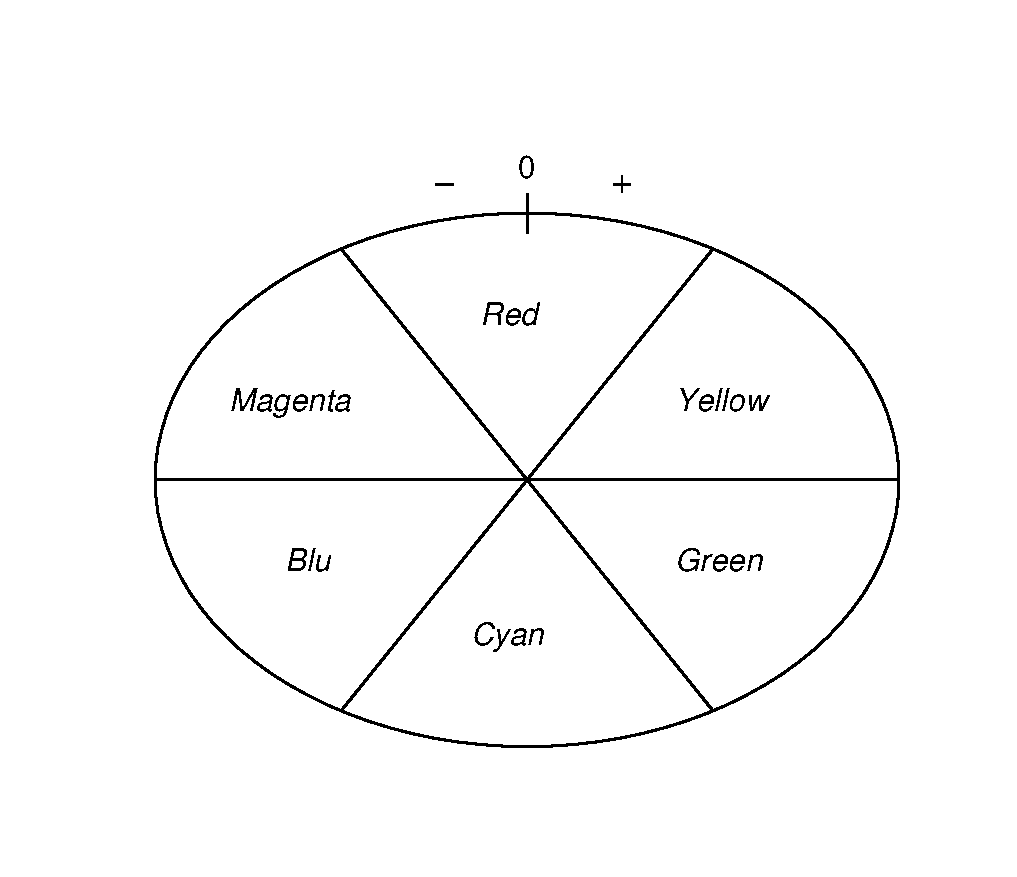
\psfig{file="./images/hsi.eps",width=5.8cm,height=5cm,bbllx=80pt,bblly=260pt,bburx=560pt,bbury=570pt,clip=}}
    \caption{Rappresentazione dello spazio della coordinata ${\it Hue}$}
    \end{figure}


    E' pu\o essere definita formalmente 
    \be
    H\,=\,\arctan\,(\,\sqrt{3}\,(\,G\,-\,B\,),2\,R\,-\,G\,-\,B\,)
    \ee
    
    che vale $0$ in presenza della sola componente monocromatica $R$.

\im (\,{\it Intensity}\,) {\it Luminosit\a}:
    \be
    I\,=\,\frac{R\,+\,G\,+\,+\,B}{3}
    \ee

    vale $0$ nel caso del colore nero ed \e massima per il bianco.

\im (\,{\it Saturation}\,) {\it Saturazione} o {\it Purezza}: misura il rapporto fra
    la componente monocromatica dominante e quella bianca necessarie ad ottenere
    il colore del punto.
    \be
    S\,=\,1\,-\,3\,\frac{\min\,\{\,R,G,B\,\}}{I}
    \ee    
    $S\,=\,1$ denota un colore puro, mentre vale $S\,=\,0$ se bianco ($R\,=\,G\,=\,B\,=\,1$).

\ei

Alternativamente alla componente $I$ si pu\o trovare la componente $V$ definita

\bi

\im {\it Value}:
    \be
    V\,=\,\max\,\{R,G,B\}
    \ee
 
\ei

%-------------------------------------------------------------------------------------
\subsection{Trasformata di Karhunen-Lo\`eve o di Hotelling}

La {\it trasformata di Karhunen-Lo\`eve o di Hotelling}, con le sue varianti, \e la trasformazione
che permette di ottenere i migliori risultati nei problemi di segmentazione  \cite{Lee},
\cite{Schmid} e di analisi della tessitura ({\it texture}) \cite{Wouver} rispetto ai diversi 
modelli di colore.
L'effetto della {\it trasformata di Hotelling} sui vettori di un dato spazio \e quello di
proiettarli in un nuovo spazio con le stesse dimensioni dove per\o ora le componenti 
risultano statisticamente scorrelate.

\vs(10)

Di seguito consideriamo la definizione della trasformazione applicata al caso di 
immagini a colori definite nello spazio $RGB$:

\vs(5)

dati i pixels ${\bf x}$ dell'immagine $I$, si considerano il vettore media e
la matrice di covarianza

\be
{\bf m}\,=\,E\,[\,{\bf x}]
\ee
\be
{\bf k}\,=\,E\,[\,(\,{\bf x}\,-\,{\bf m}\,)\,(\,{\bf x}\,-\,{\bf m}\,)^T\,]
\ee

In pratica si sostituiscono con le rispettive media e covarianza campionaria.

Si procede calcolando gli autovalori $\lambda_i$ e gli autovettori ${\bf e}_i$ della
matrice di covarianza ${\bf k}$; quindi si costruisce la matrice ${\bf A}$ le cui righe
sono gli autovettori ordinati secondo autovalori decrescenti.
La {\it trasformazione di Hotelling} \e ottenuta semplicemente
\be
{\bf y}\,=\,{\bf A}\,(\,{\bf x}\,-\,{\bf m}\,)
\lb{kltrasf}
\ee

Per verificare che le componenti degli ${\bf y}$ sono incorrelate si consideri la 
matrice di covarianza che in questo caso \e anche di correlazione in quanto sono
vettori a media nulla, infatti
\be
{\bf m_y}\,=\,E\,[\,{\bf y}]\,=\,{\bf A}\,(\,E\,[\,{\bf x}\,]\,-\,{\bf m}\,)\,=\,{\bf 0}
\lb{vmediay}
\ee
\be
{\bf k_y}\,=\,E\,[\,(\,{\bf y}\,-\,{\bf m_y}\,)\,(\,{\bf y}\,-\,{\bf m_y}\,)^T\,]
\,=\,{\bf A}\,{\bf k}\,{\bf A}^T
\lb{mcovy}
\ee

Tenendo presente che la matrice di covarianza ${\bf k}$ \e simmetrica, allora esiste
una matrice ortogonale, le cui righe formano una base ortonormale dello spazio $RGB$,
che la diagonalizza. 
La matrice ortogonale \e proprio ${\bf A}$, le cui righe sono gli autovettori di ${\bf k}$,
per cui la matrice diagonale risultante \e ${\bf k_y}$; ci\o significa che
le componenti di ${\bf y}$ sono statisticamente scorrelate e con varianza data
dagli autovalori, elementi della diagonale della matrice di covarianza.

\vs(5)

Dallo sviluppo della {\it trasformata di Hotelling} si osserva che essa permette
di scomporre l'immagine secondo le sue componenti principali valutate lungo
le direzioni a massima varianza.
Questo permette sia di limitare le trasformazioni successive alle componenti di
maggior rilievo, con un risparmio computazionale, sia di migliorare la qualit\a
delle trasformazioni successive in quanto \e possibile scartare le componenti
caratterizzate da una minor varianza (autovalori minori) che sono pi\u sensibili
al rumore (minore $SNR$).

A partire dai vettori trasformati ${\bf y}$ \e possibile riottenere i vettori
dello spazio originario ${\bf x}$ applicando la trasformazione inversa 

\be
{\bf x}\,=\,{\bf A}^{-1}\,{\bf y}\,+\,{\bf m}
\ee

con ${\bf A}^{-1}\,=\,{\bf A}^T$ per l'ortogonalit\a.

Se ora si considerano solo i primi $n$ autovettori e le prime $n$ componenti di ${\bf y}$,
si ricava

\be
\hat{\bf x}\,=\,{\bf A}^T_n\,{\bf y}_n\,+\,{\bf m}
\lb{klappr}
\ee

che rappresenta una approssimazione di ${\bf x}$.

Rilevante \e il fatto che \e possibile stabilire l'errore di approssimazione, ovvero 
la sua potenza statistica, in modo immediato data l'ortogonalit\a delle componenti.
Se $N$ \e il numero totale degli autovalori la potenza dell'errore di stima

\be
P_e\,=\,\sum_{i=n+1}^{N}\,\lambda_i
\ee

Tenendo quindi presente che gli autovalori sono ordinati in modo decrescente tale errore
risulta minimo fissato $n$.

\boss
La trasformata di Karhunen-Lo\`eve dipende, attraverso gli
autovettori della matrice di covarianza, dalle caratteristiche dell'immagine
in esame; si \e verificato per\o \cite{Ohta} che tali autovettori rimangono
pressoch\e invariati per un vasto insieme di immagini di sogetti reali.
\eoss

Quindi la trasformata si pu\o semplificare nella forma

\be
\pmatrix{K_1 \cr
         K_2 \cr
         K_3 \cr} 
\,=\,
\smatrix{3}{ \frac{1}{3} & \frac{1}{3} &  \frac{1}{3} \cr
             \frac{1}{2} &           0 & -\frac{1}{2} \cr
            -\frac{1}{2} &           1 & -\frac{1}{2} \cr}
\,
\pmatrix{R \cr
         G \cr
         B}
\ee  

Si osservi che la prima componente \e definita come l'{\it Intensit\a} in $HSI$.

%======================================================================================
\section{Operatori Morfologici}

Sono una classe importante di operatori locali che operano sulla forma degli elementi
che compaiono nell'immagine.
Gli operatori morfologici vengono utilizzati per eliminare piccoli oggetti, fessure,
buchi, regolarizzare i bordi e per individuare i bordi ({\it edge-detection}); oppure
per estrarre degli oggetti noti da un'immagine ({\it shape analysis \& pattern classification}).
 
La teoria alla base di tali trasformazioni, da cui mutuano il nome, \e la {\it matematica
morfologica} che si sviluppa a partire dalla teoria degli insiemi che assumono, in
tale contesto, un significato particolare.
In questo paragrafo si propone una breve introduzione ai due operatori base, {\it dilatazione}
({\it dilation}) ed {\it erosione} ({\it erosion}), e le due trasformazioni fondamentali,
ottenute dalle precedenti, {\it apertura} ({\it opening}) e {\it chiusura} ({\it closing}).
Per un maggior approfondimento si rimanda ai riferimenti \cite{Haralick87},\cite{Haralick92}
dello stesso autore in cui si possono trovare, oltre alle dimostrazioni, maggiori
argomentazioni sull'importanza di tali operatori e diverse indicazioni sulle possibili
applicazioni. 

\vs(5)

Di seguito si considerano le definizioni dei diversi operatori e le loro principali
propriet\a in particolare in relazione alla loro implementazione.

%-------------------------------------------------------------------------------------
\subsection{Dilatazione ed Erosione}

\bdf

Siano $A$ e $K$ due sottoinsiemi di $\M(E)^N$, si definisce {\bf dilatazione} di $A$ data $K$
\be
A\,\oplus\,K\,=\,\{\,c\,\in\,\M(E)^N\,:\,c\,=\,a\,+\,k,\,a\,\in\,A,\,k\,\in\,K\,\}
\ee

si definisce {\bf erosione} di $A$ dato $K$
\be
A\,\ominus\,K\,=\,\{\,c\,\in\,\M(E)^N\,:\,c\,+\,k\,\in\,A,\,\forall\,k\,\in\,K\,\}
\ee

\edf

\boss
In generale i termini $A$ e $K$ sono due generici sottoinsiemi dello spazio $\M(E)^N$,
in realt\a il primo operando \e l'immagine che si sta elaborando mentre il secondo
costituisce il nucleo o elemento strutturale ({\it structuring element}) della 
trasformazione rappresentante un parametro di forma di un elemento dell'immagine.
\eoss

Per implementare in modo pi\u efficiente i due operatori \e opportuno esprimerli come 
combinazioni dell'immagine traslata

\bdf
Dati $A\,\subseteq\,\M(E)^N$, $x\,\in\,\M(E)^N$, si definisce traslazione di $A$ dato $x$
\be
A_x\,=\,\{\,c\,\in\,\M(E)^N\,:\,c\,=\,a\,+\,x,\,a\,\in\,A\,\}
\ee
\edf

\bpr
\be
A\,\oplus\,K\,=\,\bigcup_{k \in K}\,A_k
\lb{tr_dil}
\ee

\be
A\,\ominus\,K\,=\,\bigcap_{k \in K}\,A_{-k}
\ee
\epr

\bpr
 Gli operatori di {\it dilatazione} ed {\it erosione} soddisfano le seguenti propriet\a:

\bi

\im {\bf Commutativa}. Vale solo per l'operatore di {\it dilatazione}. 
    \be
    A\,\oplus\,K\,=\,K\,\oplus\,A 
    \lb{com_dil}
    \ee

\im {\bf Associativa}. Sia $K\,=\,K_1\,\oplus\,K_2$
    \beqa
    \lb{assde}
    A\,\oplus\,K & = & A\,\oplus\,(\,K_1\,\oplus\,K_2\,)\,=\,(\,A\,\oplus\,K_1\,)\,\oplus\,K_2 \\
    A\,\ominus\,K & = & A\,\ominus\,(\,K_1\,\ominus\,K_2\,)\,=\,(\,A\,\ominus\,K_1\,)\,\ominus\,K_2 \nonumber
    \;\;\;\;\;\;\;\;
    \eeqa
    
\im {\bf Distributiva}.

    Fra le possibili combinazioni si considerano in particolare
    \beqa
	\lb{dist}    
    A\,\oplus\,(\,B\,\cup\,C\,) & = & (\,A\,\oplus\,C)\,\cup\,(\,A\,\oplus\,C\,) \\
    %-------------------------------------------------------------------------------   
    A\,\ominus\,(\,B\,\cup\,C\,) & = & (\,A\,\ominus\,C)\,\cap\,(\,A\,\ominus\,C\,) \nonumber
    \eeqa

\ei    
\epr

\boss
Dalle (\ref{assde}) e (\ref{dist}) si possono ricavare due
soluzioni per scomporre il nucleo della tarsformazione ({\it structuring element});
la differenza \e che nelle (\r{assde}) si ottiene una cascata di operazioni elementari
mentre nelle (\r{dist}) tali operazioni sono eseguibili in parallelo.
\eoss

Esiste anche un teorema di dualit\a che lega i due operatori.

\bth
{\bf Dualit\a.}

$$
(\,A\,\ominus\,B\,)^c\,=\,A^c\,\oplus\,\check{B} 
$$

dove $\check{B}\,=\,\{\,x\,:\,\exists\,b\,\in\,B\,:\,x\,=\,-\,b\,\}$

e $(\,^c\,)$ \e l'usuale operazione di complemento rispetto l'insieme $\M(E)^N$.
\eth

Il teorema mette in luce il fatto che le due operazioni non sono l'una l'inversa
dell'altra nel senso usuale del termine, ma si possono considerare complementari.
Nel senso che se si considera la dilatazione di un insieme $A\,\subseteq\,\M(E)^N$,
\e possibile in modo duale ottenere lo stesso risultato con un'operazione di
erosione sull'insieme complementare.
In particolare nel caso in cui il nucleo ({\it structuring element}) sia simmetrico,
per cui $\check{K}\,=\,K$, si ha che l'erosione di $A$ dato $K$ \e perfettamente
complementare alla dilatazione di $A^c$ dato $K$.

\vs(5)

Prima di introdurre i due operatori fondamentali della matematica morfologica
\e opportuno considerare il seguente risultato

\bpr

$$
A\,\oplus\,(\,B\,\ominus\,C\,)\,\subseteq\,(\,A\,\oplus\,B\,)\,\ominus\,C
$$

\epr

che evidenzia l'importanza dell'ordine di applicazione dei due operatori {\it dilatazione}
ed {\it erosione}.

%-------------------------------------------------------------------------------------
\subsection{Apertura e Chiusura}

In pratica le due operazioni considerate nella sezione precedente non sono quasi mai
utilizzate singolarmente ma combinate per realizzare le due trasformazioni fondamentali 
di {\it apertura} ({\it opening}) e {\it chiusura} ({\it closing}).

\bdf

Si definisce {\bf apertura} di $A$ dato $K$

\be
A\,\circ\,K\,=\,(\,A\,\ominus\,K\,)\,\oplus\,K.
\ee

Se $A\,\circ\,K\,=\,A$ si dice che $A$ \e {\bf aperto} rispetto $K$.

Si definisce {\bf chiusura} di $A$ dato $K$

\be
A\,\bullet\,K\,=\,(\,A\,\oplus\,K\,)\,\ominus\,K.
\ee

Se $A\,\bullet\,K\,=\,A$ si dice che $A$ \e chiuso rispetto $K$.

\edf

Una propriet\a importante dei due operatori \e l'idempotenza.

\bth
{\bf Idempotenza.}
\beqa
(\,A\,\circ\,K\,)\,\circ\,K & = & A\,\circ\,K \\
(\,A\,\bullet\,K\,)\,\bullet\,K & = & A\,\bullet\,K \nonumber
\eeqa
\eth

Vale anche una relazione di dualit\a da intendersi come per i due operatori precedenti. 

\bth
{\bf Dualit\a.}
\be
(\,A\,\bullet\,K\,)^c\,=\,A^c\,\circ\,\check{K}
\ee
\eth

Un'interpretazione geometrica dell'azione dei due operatori \e data dal seguente risultato.

\bpr

\be
A\,\circ\,K\,=\{\,x\,\in\,A\,:\,\exists\,y\,:\,x\,\in\,K_y\,\subseteq\,A\,\}
\,=\,\bigcup_{\{y\,:\,K_y\subseteq\,A\}}\,K_y
\ee

\epr

Esprime l'operazione di {\it apertura} come l'unione di tutte le possibili traslazioni
di $K$ che sono contenute in $A$.

Sfruttando la dualit\a si ha invece che l'operazione di {\it chiusura} \e otenuta
come il complemento dell'unione di tutte le traslazioni di $\check{K}$ contenute
in $A^c$.

%-------------------------------------------------------------------------------------
\subsection{Operatori morfologici per immagini binarie}

Nel caso particolare di immagini binarie gli operatori morfologici si riducono ad
espressioni logiche a cui \e possibile applicare le regole dell'algebra di Boole.

Si consideri l'operazione di {\it dilatazione} espressa nella forma (\r{tr_dil}) con
$A$, il sottoinsieme che definisce gli oggetti presenti e i cui pixels assumono valore $1$
({\it foreground}), e $K$ che assume valori in $\{0,1\}$; allora

$$
A\,\oplus\,K\,=\,\bigcup_{k\,\in\,K}\,A_k\,=\,\bigcup_{a\,\in\,A}\,K_a
$$

dove nell'ultimo passagio si \e sfruttata la commutativit\a dell'operatore (\r{com_dil}).

La {\it dilatazione} \e quindi ottenuta centrando la maschera $K$ su tutti i pixel
di $A$ e commutando ad $1$ tutti i pixels vicini che assumono eventualmente il
valore $0$ appartenenti a $A^c$ ({\it background}).

Tale operazione pu\o essere realizzata considerando gli operatori logici $and\,\wedge$ e
$or\,\vee$ tra l'immagine $I\,\supseteq\,A$ e la maschera $K$. Nell'ipotesi verosimile
che quest'ultima sia definita da una finestra-matrice simmetrica di dimensioni 
$(\,2\,n\,+\,1,2\,n\,+\,1\,)$ si ricava

\be
\hat{I}\,(\,r,c\,)\,=\,\bigvee_{i\,=\,-n}^{n}\,\bigvee_{j\,=\,-n}^{n}
\,K\,(\,i,j\,)\,\wedge\,I\,(\,r\,-\,i,c\,-\,j\,)
\ee

A questo punto \e possibile ottenere un'espressione anche per l'{\it erosione} sfruttando
la dualit\a e tenedo conto che $K$ \e simmetrica per cui $\check{K}\,=\,K$ e che
il complemento \e dato dalla negazione

\be
\hat{I}\,(\,r,c\,)\,=\,\overline{\bigvee_{i\,=\,-n}^{n}\,\bigvee_{j\,=\,-n}^{n}
\,K\,(\,i,j\,)\,\wedge\,\overline{I\,(\,r\,-\,i,c\,-\,j\,)}}
\ee

Definiti questi due operatori \e possibile ottenere per composizione anche quelli
pi\u complessi.

%-------------------------------------------------------------------------------------
\subsection{Operatori morfologici per immagini in scala di grigio}

Anche in questo caso le espressioni viste in generale assumono una forma pi\u
semplice una volta che si \e stabilito di lavorare con immagini a toni di grigio.
Lo spazio considerato \e $\M(E)^N\,=\,\M(E)^3$ dove le prime due componenti di ciascun
vettore sono le coordinate del punto dell'immagine mentre la terza rappresenta
il valore dell'intensit\a dell'immagine nel punto.

Per le immagini in scala di grigio le due operazioni che permettono di definire
la {\it dilatazione} e l'{\it erosione} sono quelle di {\it massimo} e {\it minmo}
rispettivamente

\bpr

Siano $F,K\,\subseteq\,\M(E)^2$, $f\,:\,F\,\rightarrow\,\M(E)$ e $k\,:\,K\,\rightarrow\,\M(E)$

\beqa
(\,f\,\oplus\,k\,)(\,x\,) & = & \max_{\matrix{\scriptstyle{\{\,y\,\in\,K,}\cr\scriptstyle{x\,-\,y\,\in\,F\,\}}}}\,
\{\,f\,(\,x\,-\,y\,)\,+\,k\,(\,y\,)\,\} \\
(\,f\,\ominus\,k\,)(\,x\,) & = & \min_{\{\,y\,\in\,K\,\}}\,
\{\,f\,(\,x\,+\,y\,)\,-\,k\,(\,y\,)\,\} \nonumber
\eeqa

\epr
 
Da cui \e possibile ottenere tutti gli altri operatori applicando le definizioni
date precedentemente.

%======================================================================================
\section{Rank-order filters - Mediana}

Rappresentano una classe di operatori locali non lineari che dipendono dal-l'ordinamento
dei valori definiti in una finestra $K\,(\,n,n\,)$, con $n$ dispari, centrata su ogni pixel
dell'immagine $I\,(\,R,C\,)$.

A partire da ${\bf v}_K$, vettore ordinato con valori crescenti, si possono ottenere
$n^2$ possibili risultati associati ai ${\bf v}_K\,(i)$, con $i$ ordine del filtro,
assegnabili al pixel centrale, oggetto dell'elaborazione. 

Se $i=1$ si ha il $min$, con $i=n^2$ il $max$ e con $i=(n^2+1)/2$ la
$mediana$ del vettore, che presenta alcune propriet\a interessanti \cite{Zamperoni}
e \cite{Haralick92}.

\boss
Nella costruzione del vettore ${\bf v}_K$ si \e considerato anche il pixel centrale
della finestra mentre in letteratura si possono trovare anche altre formulazioni che lo escludono.
In questi casi bisogna fare attenzione che se $n$ \e dispari allora $n^2-1$, il numero
di elementi del nuovo vettore ${\bf v}_K^\prime$, \e pari e si hanno due possibili valori
di mediana per $i=(n^2-1)/2$ e $i=(n^2-1)/2+1$. 
\eoss

I {\it rank-order filters} in generale e l'{\it operatore mediana} in particolare, con 
le loro varianti, vengono utilizzati sia per ridurre il rumore presente nell'immagi-ne
({\it image enhancement}) sia come componente per l'estrazione di particolari 
caratteristiche ({\it features}) dell'immagine, quali pattern lineari.
 
%======================================================================================
\section{Misura dell'anisotropia locale}

Bisogna considerare che all'interno di immagini, soprattutto quelle naturali, vi sono
particolari con caratteristiche spesso molto diverse tra di loro.

La possibilit\a di adattare l'operatore alle propriet\a locali dell'immagine permette di
soddisfare delle condizioni che potrebbero risultare altrimenti incompatibili, come 
ridurre il rumore e contemporaneamente conservare o migliorare la definizione dei bordi
({\it edge sharpness}) e dei dettagli.

Bisogna a questo punto definire uno o pi\u parametri che caratterizzino il comportamento del
filtro nei diversi punti dell'immagine.
Ci\o viene realizzato attraverso una {\it misura di anisotropia} che rivela la propriet\a di interesse
come, ad esempio, i punti appartenenti ai bordi (si veda il caso della {\it diffusione anisotropa}
ottenuta variando la forma del filtro gaussiano,
che \e per sua natura isotropo, in funzione del gradiente dell'immagine \cite{Perona}, \cite{Fischl}).  

\vs(5)

Una semplice definizione di anisotropia \e data dalla funzione $\alpha(p)$, misura di anisotropia nel
punto $p$, che stabilisce se il punto $p$ appartiene ad una regione uniforme, $\alpha(p)=0$,
o a una retta (pattern lineare filiforme e ben definito rispetto allo sfondo), $\alpha(p)=1$.

\bdf
Definita una finestra $K(\,n,n\,)$, con $n$ dispari, centrata sul pixel $p$, \e possibile
individuare $T=2\,(n-1)$ {\bf digital straight line segments} passanti per il punto $p$ e che
connettono due punti del bordo della finestra $K$ come in figura (\r{digseg}).
%(L'algoritmo che costruisce tali segmenti \e riportato in Appendice).
Si consideri $M_t$, con $t=1,\dots,T$, la media dell'intensit\a $I(x,y)$ lungo il segmento 
$t-esimo$ moltiplicato per $n$
\be
M_t\,=\,\sum_{i=-z}^{z}\,I\,(\,x+dx(t,i),y+dy(t,i)\,), \qquad z=(n-1)/2
\ee

dove $dx(t,i)$ e $dy(t,i)$ contengono gli spostamenti relativi tra il punto $p(x,y)$ su cui
\e centrata la finestra e i punti appartenenti alla retta $t-esima$.

Si definiscono ora $m_K(p)$ e $M_K(p)$
\bary(2)
m_K(p)\,=\,{\displaystyle{\min_{\matrix \scriptstyle t=1,\dots,T}}}\,\{\,M_t\,\} \quad
 & M_K(p)\,=\,{\displaystyle{\max_{\matrix \scriptstyle t=1,\dots,T}}}\,\{\,M_t\,\} 
\eary

A questo punto \e possibile definire la misura $\alpha(p)$ dell'anisotropia locale
\[
\alpha(p)=\cases{0 & se $M_K(p)=0$ \cr
                 {\displaystyle\frac{M_K(p)-m_K(p)}{M_K(p)+m_K(p)}} & altrimenti. \cr}
\lb{lam}
\]
 
\edf

\begin{figure}[tbp]
 \centerline{
  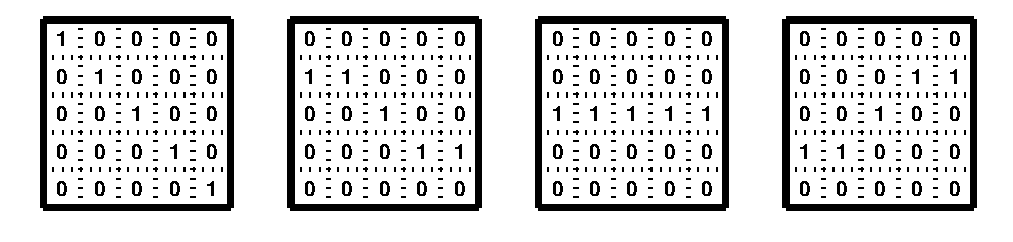
\psfig{file="./images/digseg1.eps",height=3cm,bbllx=80pt,bblly=350pt,bburx=550pt,bbury=450pt,clip=}}
 \centerline{
  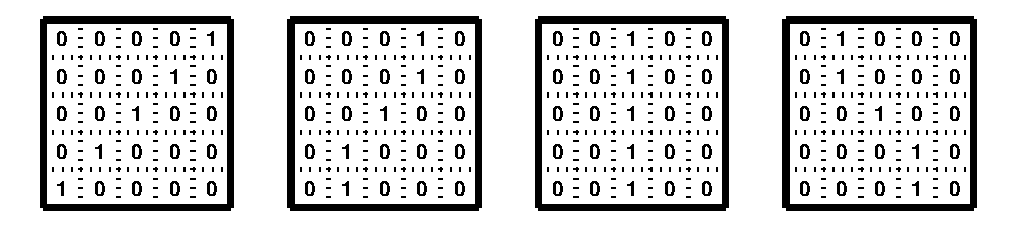
\psfig{file="./images/digseg2.eps",height=3cm,bbllx=80pt,bblly=350pt,bburx=550pt,bbury=450pt,clip=}}
 \caption[Digital straight line segments]
  {Gli $2\,(n-1)=8$ possibili {\it digital straight line segments} distinti passanti per il
   pixel $p$, al centro della maschera $K(n,n)$, nel caso di $n=5$}
 \lb{digseg}
\end{figure}

\finepar
 







% Segmentazione
\chapter{Segmentazione}\lb{SGM}

Il processo di segmentazione ha come risultato finale la ripartizione dell'im-magine in
unit\a morfologiche, segmenti, disgiunte fra loro.
Questo pu\o essere ottenuto determinando i bordi di tali segmenti oppure raggruppando
i pixels (unit\a elementari) in regioni omogenee rispetto ad una particolare propriet\a
({\it feature}) fissata che pu\o essere il colore e/o la tessitura ({\it texture}).

%======================================================================================
\section{Caratterizzazione della segmentazione}

Formalmente la segmentazione pu\o essere definita
\bdf
Dati l'insieme $I$, che definisce nel nostro caso l'immagine da analizzare, e il
predicato di omogeneit\a $\cal O$, la segmentazione di $I$ dato $\cal O$ \e una
partizione $\cal P$ di $I$ in $N$ sottoinsiemi, o regioni, $R_i$ tali che
\ben
\im \quad ${\displaystyle \bigcup_{i=1}^{N}\,R_i\,=\,I}
     \qquad R_i\,\cap\,R_j\,=\,\emptyset \quad \forall\,i\,\neq\,j$

\im \quad ${\cal O}(R_i)\,=\,true \quad \forall\,i$

\im \quad ${\cal O}(R_i\,\cup\,R_j)\,=\,false \quad \forall\,R_i,R_j \quad adiacenti$
\een
 
\edf

La prima \e propria della definizione di partizione; pi\u interessanti le altre due
che stabiliscono che ciascuna regione \e omogenena rispetto $\cal O$ e soprattutto
che a conclusione della segmentazione le regioni adiacenti devono necessariamente essere
diverse tra loro, al contrario sarebbe possibile unirle con una
ulteriore semplificazione della rappresentazione della stessa immagine $I$.

%======================================================================================
\section{Tecniche di segmentazione}

Seguendo la classificazione data in \cite{Lucchese} le tecniche di segmentazione possono
essere suddivise nel seguente modo
\ben
\im Tecniche definite sullo spazio delle primitive ({\it features}).\par
    ({\sl Feature-Space Based Techniques}) 
    \ben
    \im Clustering \& Adaptive k-means Clustering
    \im Histogram Thresholding
    \een
\im Tecniche definite sull'intera morfologia dell'immagine.\par
    ({\sl Image-Domain Based Techniques})
    \ben
    \im Split \& Merge
    \im Region Growing
    \im Edge Based
    \im Neural-Network Based Classification
    \een
\im Tecniche che tengono conto della fisica dell'interazione tra la luce e le 
    superfici dei materiali.\par 
    ({\sl Physics Based Techniques})
\een 

Anche se la classificazione in \cite{Lucchese} \e definita in relazione alle tecniche
che considerano l'informazione ricavata dal solo {\it colore} delle superfici, 
\e possibile estenderla anche al caso in cui si consideri la tessitura
({\it texture segmentation}).


%--------------------------------------------------------------------------------------
\subsection{Feature-Space Based Techniques}\lb{ftdom}

Nell'ipotesi che ciascun elemento dell'immagine sia omogeneo e definito da una ben nota
primitiva ({\it feature}) \e possibile raggruppare i pixels che la soddisfano considerandoli 
come un'unica unit\a ({\it cluster}).
Alternativamente \e possibile costruire un particolare istogramma, definito nello spazio
delle {\it features}, e dalla sua analisi determinare uno o pi\u valori di soglia 
({\it binarization \& multilevel thresholding}) che suddividono lo spazio in un certo
numero di classi.

Il difetto di tali approcci \e che non tengono in conto la morfologia dei clusters 
individuati trascurando le relazioni spaziali di vicinanza fra le features.
A causa dei disturbi dovuti alle condizioni di illuminazione \e probabile che si abbiano
i clusters principali non compatti e ben definiti, come dovrebbero risultare, ma interroti da
altri clusters piccoli o piccolissimi che possono complicare o falsare i successivi
passi di analisi e riconoscimento degli oggetti visualizzati.

%--------------------------------------------------------------------------------------
\subsection{Image-Domain Based Techniques}\lb{imdom}

Per garantire anche quest'ultima condizione di compattezza \e necessario introdurre delle 
condizioni che tengano conto della distribuzione spaziale delle features.

% .  .  .  .  .  .  .  .  .  .  .  .  .  .  .  .  .  .  .  .  .  .  .  .  .  .  .
\subsubsection{Tecniche di Split \& Merge e Region Growing}

Le prime suddividono ricorsivamente ({\it split}) l'immagine in unit\a sempre pi\u piccole
fino ad ottenere una partizione omogenea; successivamente procedono alla
fusione ({\it merge}) di clusters vicini, appartenenti in generale a due rami differenti
della ripartizione, che si possano considerare omogenei fra loro.

Le seconde invece partono dalla definizione di alcuni nuclei iniziali, {\it semi} e
progressivamente li accrescono agglomerando i punti vicini che soddisfano il criterio
di prossimit\`a, o omogeneit\a, fissato.

In entrambe le classi di algoritmi \e rilevante la scelta del criterio
di omogeneit\a, il predicato $\cal O$, che generalmente viene definito come 
funzione che misura la distanza fra le classi in relazione alla {\it distribuzione delle
features al loro interno} \cite{Puzicha}.
Nello stesso articolo \e sottolineato il fatto che non \e possibile stabilire una
misura che sembri offrire delle prestazioni superiori alle altre in ogni applicazione,
ma che comunque alcune si comportano meglio in determinate ipotesi di lavoro.
Nel caso della segmentazione risulta che la scelta mediamente  soddisfacente
in termini di errore di ripartizione \e la $\chi^2-statistics$.

Inoltre nel caso delle tecniche ad accrescimento tipo {\it region growing} \e problematica
anche la decisione dei punti di aggregazione iniziali i quali possono essere fissati
in corrispondenza dei punti di minimo del modulo del gradiente del colore dell'immagine, a cui
corrispondono regioni abbastanza uniformi, oppure realizzando una opportuna quantizzazione
dei colori presenti, o pi\u semplicemente distribuendo i semi in modo uniforme.

% .  .  .  .  .  .  .  .  .  .  .  .  .  .  .  .  .  .  .  .  .  .  .  .  .  .  .
\subsubsection{Tecniche basate sulla rilevazione dei bordi ({\it Edge})}\lb{imedg}

Alla stessa classe di algoritmi appartengono quelli che realizzano la segmentazione
individuando i bordi ({\it edge}), cio\e l'insieme dei punti di transizione,
e quindi a maggior contrasto, fra una regione omogenea e l'altra.
Nel caso di immagini scalari, in cui \e presente la sola componente di intensit\`a, esistono 
diversi algoritmi ottenuti applicando all'immagine un opportuno operatore, Sobel, Kirsch,
pseudo-Laplace, LoG (Mexican-hat), morfologici \cite{Zamperoni} o il pi\u noto filtro di
Canny \cite{Canny} che rappresenta il filtro lineare ottimo, nel caso unidimensionale e con 
rumore gaussiano bianco, che soddisfa le seguenti condizioni
\ben
\im bassa probabilit\a di mancare un buon edge e bassa probabilit\a di considerare
    vero un falso edge; ovvero massimizzare l'$SNR$ in uscita al filtro;
\im corretta localizzazione dell'edge.
\een 
Il risultato \e un filtro le cui prestazioni possono essere ottenute, con buona
approssimazione, anche dalla derivata prima, $G_{\sigma}^{\,\prime}\,(x)$, della gaussiana
$$
G_\sigma(x)\,=\,\frac{1}{\sigma\,\sqrt{2\,\pi}}\exp\,\Big(\,-\,\frac{x^2}{2\,\sigma^2}\,\Big);
$$
e quindi gli edges sono determinati dalla convoluzione 
$$
C(x)\,=\,G_{\sigma}^{\,\prime}(x) \ast I(x)\,=\,(\,G_{\sigma} (x) \ast I(x)\,)^{\,\prime}
$$
per le propriet\a del filtro gaussiano.

\vs(5)

L'estensione al caso bidimensionale \e ottenuta tenendo presente che si deve ora considerare
il gradiente di $G_\sigma (x,y)$
$$
C(x,y)\,=\,\nabla G_\sigma \ast I\,=\,\nabla (\,G_\sigma \ast I\,)\,=\,
 \nabla (\,G_\sigma (x) \ast (\,G_\sigma (y) \ast I\,)\,)
$$
dove le ultime due uguaglianze sono valide ancora per le prorpiet\a della gaussiana.

Noto $C$ \e possibile determinare l'orientazione dell'{\it edgel} (edge element)
dalle componenti di $C\,/\,|C|$ mentre la sua altezza dal modulo $|C|$.

E' possibile che fra gli {\it edgel} determinati ve ne siamo molti non desiderati dovuti
ad esempio alla tessitura delle superfici o ad altri disturbi che non sono eliminati
dalla convoluzione col filtro passa basso $G_\sigma$.
Si potrebbe pensare di poter aumentare la scala $\sigma$, ma ci\o vorrebbe dire
ridurre la capacit\a di localizzazione degli edge; invece si fissa un valore di soglia
per la scala utilizzata in modo da scartare gli edge che hanno un'intensit\a inferiore.

Il problema appena individuato \e dovuto alla due condizioni strutturali rispetto le quali
\e stato definito il filtro e che non possono essere soddisfatte contemporaneamente; 
infatti una migliore realizzazione della prima porta un degrado della seconda, e viceversa.
La scelta dei parametri \e quindi frutto di un compromesso ({\it trade-off}) fra le due.

Esistono inoltre delle situazioni in cui il filtro di Canny pu\o fallire:
\bi
\im nel caso di un'area dell'immagine con un gradiente di intensit\a che \e costante
    ma non nullo il filtro pu\o decidere per la presenza di edges quando invece non
    dovrebbero esserci;
\im se si \e in presenza di edge composito, per esempio gradino pi\u rampa,
    si ha un errore sistematico nella localizzazione dell'edge stesso;
\im non riesce ad individuare le giunzioni a $T$ che si hanno quando tre regioni 
    distinte e adiacenti l'una all'altra.
\ei
 
Una delle cause dei problemi appena menzionati \e la natura lineare del filtro; infatti
\e mostrato in \cite{Perona90} che per ogni famiglia finita di filtri lineari esiste
un {\it edgel} composito per cui le risposte presentano un errore sistematico.
Sempre in \cite{Perona90} \e fornita la soluzione al problema che \e data dalla
scelta di una diversa classe di filtri ottenuti come combinazione di filtri
in quadratura tra loro.
Dalla convoluzione tra questi e l'immagine, ed elevando al quadrato il modulo, si ottiene
una forma quadratica che individua l'{\it edgel} nel suo punto di estremo.
Tale forma quadratica dipende anche dalla fase e quindi l'estremo determinato permette
di definire l'orientazione dell'{\it edgel} in modo pi\u preciso rispetto al caso precedente,
con una risoluzione che \e possibile stabilire a priori.
Un altro grado di libert\a \e dato dalla forma della coppia di filtri che \e vincolabile
fissando un criterio che condizioni gli {\it edgel} risultanti: un elevato $SNR$, come
nel caso di Canny, minima varianza dell'errore di localizzazione, bassa probabilit\a
di {\it edgel} multipli (cio\e falsi {\it edgel} dovuti al ripple del filtro e che si affiancano
a quelli veri), etc.

\vs(5)

Nel caso delle immagini a colori si possono applicare gli stessi metodi previa l'estensione
della nozione di gradiente nel caso di immagini vettoriali che \e realizzabile in due
modi:
\ben
\im calcolare per ciacuna componente il gradiente e quindi combinare opportunamente
    i risultati parziali;
\im definire l'estensione del calcolo del gradiente per funzioni vettoriali
    \cite{Gevers}, \cite{Lucchese}

    Sia definita l'immagine 
    $$
    {\bf \Psi}({\bf x}):\,\M(R)^2\,\longrightarrow\,\M(R)^N
    $$
    la variazione di ${\bf \Psi}({\bf x})$, $d{\bf \Psi}$, per uno spostamento infinitesimo
    $d{\bf x}$ \e espressa dalla forma differenziale
    $$
    d{\bf \Psi}\,=\,\frac{\,\partial {\bf \Psi}}{\partial x}\,dx\,+
                  \,\frac{\,\partial {\bf \Psi}}{\partial y}\,dy
    $$
    la cui norma al quadrato risulta
    $$
    d{\bf \Psi}^2\,=\,d{\bf x}^T\,G\,d{\bf x}
    $$
    dove $G$ \e una matrice $(2 \times 2)$ le cui componenti sono 
    $$
    g_{ij}\,=\,\frac{\partial {\bf \Psi}}{\partial x_i}
             \,\frac{\partial {\bf \Psi}}{\partial x_j}.
    $$
    Le direzioni di estremo della forma quadratica sono definite dagli autovettori di $G$, 
    mentre gli autovalori associati stabiliscono l'altezza del-l'estremo; quindi
    riferendoci all'immagine di partenza, gli autovettori indicano le direzioni di massima
    e minima variazione, mentre gli autovalori l'entit\a della variazione rispetto al
    punto {\bf x}.
    
    \vs(5)
 
    {\sl La ripidit\a ({\it sharpeness}) dell'immagine nel punto, ovvero il "{\it gradiente}",
    pu\o essere definito dalla radice quadrata della differenza dei due autovalori;
    cos\iac\,\,facendo si \e ottenuto in una sola misura l'informazione sulle variazioni
    di grandezza vettoriali}.
\een

Rispetto all'immagine originale costituita da tutti i suoi {\it pixels}, \e quindi possibile
ottenere una rappresentazione pi\u compatta considerando gli {\it edgels} ricavati con
uno degli edge-detector menzionati.
Il grado di compressione risulta dipendente dall'immagine considerata in quanto
vi possono essere comunque un numero elevato di elementi in base anche alla scelta del
valore di soglia fissato; inoltre la rappresentazione non tiene conto della possibile
continuit\a degli edgels, rendendo difficoltosa l'interpretazione degli oggetti, o di
loro parti, individuati.

Per ovviare a questo inconveniente si pu\o ricorrere ad un'altra classe di modelli 
denominati {\bf active contours} o {\it snakes}, originalmente proposti da Kass \cite{Kass}
e rielaborati nel caso particolare delle immagini a colori nei {\it color snakes} \cite{Gevers}
dove si sfrutta la definizione data sopra sul calcolo del gradiente
per immagini vettoriali.

\vs(5)

{\sl Tale modello rappresenta uno degli elementi fondamentali dell'algoritmo proposto in
questa tesi e sar\a perci\o approfondito nei prossimi capitoli}.

% .  .  .  .  .  .  .  .  .  .  .  .  .  .  .  .  .  .  .  .  .  .  .  .  .  .  .
\subsubsection{Tecniche di classificazione basate sulle reti Neuronali}

Una rete neuronale \cite{Bose} \e costituita da uno o pi\u strati ({\it multi-layer}), esclusi
quello d'ingresso e quello di uscita, di celle elementari, i {\it neuroni}.
Ciascun neurone \e costituito da due elementi: il primo, denominato {\it adaptive linear
combiner}, riceve in ingresso i segnali provenienti dai neuroni dello strato che
lo precede e li combina linearmente secondo dei coefficienti, {\it pesi sinattici};
mentre il secondo \e una particolare funzione, {\it legge di attivazione} che elabora
il risulato della combinazione determinando il nuovo stato del neurone, che rappresenta
l'uscita che si propaga agli strati successivi.
Esempi di leggi di attivazione sono la funzione segno, la rampa lineare, la sigmoide 
\footnote{$1/(1+\exp(-k\,x))$}, etc.

Il vantaggio di presentare una struttura intrinsecamente parallela, che pu\o risultare
determinante in termini di tempo di calcolo, oltre ad un buon comportamento nei confronti
dei disturbi, \e controbilanciato dallo svantaggio di richiedere una fase di
apprendimento ({\it learning}) in cui vengono adattati i pesi sinattici in relazione alle
caretteristche del {\it pattern} in esame. 

Esistono due tipi principali di apprendimento:
\bi
\im {\it supervisionato}: deve essere disponibile una collezione, {\it training set},
     di coppie $I/O$. Le leggi di apprendimento sono definite in modo che sia
     minimo l'errore in uscita fra il valore desiderato e quello reale fornito
     dalla rete, una volta fissati i pesi.\par 
     Gli algoritmi si suddividono quindi in {\it algoritmi a correzione d'errore}
     ($\alpha-LMS$ o Widrow-Hoff Delta, MRI, MRII) e {\it algoritmi a discesa lungo il
     gradiente dell'errore} ($\mu-LMS$, Back-Propagation) sviluppati in base al tipo di 
     rete (single-layer, AdaLinE o multi-layer, M-AdaLinE). 
\im {\it senza supervisione}: in questo caso non \e disponibile un insieme di prova
    ma \e la rete che aggiorna il suo comportamento in relazione al tipo di ingressi.
    Si realizza una struttura basata su rapporti di associazione tra un dato tipo
    di ingresso \e una quota di neuroni che risultano particolarmente attivi quando
    questi si presenta e che \e fissata incrementando il valore dei rispettivi pesi
    sinattici.
    Uno dei modelli di rete che utilizza questo tipo di apprendimento \e dato dalle
    reti di Kohonen o $SOM$ ({\it Self Organizing Map}). 
\ei

Un'altra importante tipologia di reti \e data dalle {\it reti di Hopfield} che presentano 
carateristiche peculiari:
\bi
\im a differenza dei modelli precedenti in cui i segnali si propagano in una sola
    direzione dall'ingresso verso l'uscita ({\it feed-forward}), queste presentano
    anche dei collegamenti in retroazione ({\it feed-back}) dato che ciascun nodo
    della rete, il neurone, \e collegato con tutti gli altri ({\it fully-connected});
    per cui non \e pi\u possibile una organizzazione a strati;
\im una volta annullato l'ingresso l'evoluzione dello stato del neurone pu\o raggiungere
    una condizione di equilibrio stabile, con l'esaurimento del transitorio, oppure rimanere
    in uno di stato di instabilit\a con oscillazioni permanenti;
\im vengono utilizzate nella risoluzione di problemi di ottimizzazione 
    nella minimizzazione di {\it funzioni costo} che possono, nel nostro caso,
    rappresentare dei vincoli per la segmentazione.
    In particolare i minimi di tali funzioni corrispondono agli stati finali stabili,
    o attrattori stabili, della rete.
\ei
    
%--------------------------------------------------------------------------------------
\subsection{Physics Based Techniques}

Sostanzialmente non differiscono dalle precedenti se non nel fatto che inseriscono
dei termini che tengano conto del comportamento fisico delle superfici dei materiali,
in termini di riflessione, al variare delle condizioni di illuminazione.
Pu\o risultare infatti che la superficie di uno stesso materiale, caratterizzata
da un solo colore, pu\o apparire invece non uniforme con possibili problemi di
sovrasegmentazione in quanto si individuano pi\u regioni di quelle reali.
In generale i materiali sono suddivisi in tre categorie: dielettrici otticamente omogenei,
dielettrici otticamente non omogenei e metalli; per ciasuna delle quali \e definibile
un modello che rappresenti i fenomeni di riflessione della superficie che determinano il
colore percepito.
Tali modelli tengono conto della geometria e del tipo di superficie, della posizione relativa
sorgente-soggetto, della natura della sorgente (la lunghezza d'onda della luce emessa)
ovvero se sia luce bianca o abbia delle componenti monocromatiche prevalenti.
In alcuni casi permettono di determinare le diverse componenti di riflessione dovuti
anche alle interazioni fra gli oggetti presenti fra cui necessariamente il sensore che
effettua la misura. 

%======================================================================================
\section{Texture segmentation}

Come accennato precedentemente le tecniche utilizzate nella segmentazione sono valide
sia che si consideri il solo colore sia che si consideri la tessitura ({\it texture})
sia che vengano utilizzate entrambe.

A differenza del colore che \e una propriet\a puntuale, la tessitura da una descrizione
locale delle relazioni spaziali fra pixel vicini; inoltre dipende dalla scala 
utilizzata, ovvero ad un determinato livello di risoluzione alcuni dettagli possono non
essere presenti mentre lo sono se la si aumenta, come se si analizzasse la stessa superficie 
a diversi gradi di ingrandimento.

Per cui gli algoritmi di analisi della tessitura fanno largo utilizzo di metodi
a multirisoluzione con strutture tipo {\it piramide di immagini} a cui sono applicate
filtri la cui forma dipende dalla scala del livello.

Vista la caratteristica che devono avere i filtri una delle scelte comunemente adottate
\e data dal filtro gaussiano $G_\sigma$, il cui fattore di forma \e dato dalla sua varianza,
oppure, per problemi pi\u complessi, dalla famiglia di filtri complessi che vanno sotto
il nome di {\it filtri di Gabor}
$$
G_\sigma({\bf x},{\bf k})\,=\,\frac{1}{\sigma\,\sqrt{2\,\pi}}
                           \exp\,\Big(\,-\,\frac{{\bf x}^T\,{\bf x}}{2\,\sigma^2}\,\Big)
                           \exp\,\Big(\,{\mit i}\,{\bf k}^T\,{\bf x}\,\Big)
$$
con $\sigma$ funzione di ${\bf k}$, il pararmetro che caratterizza la feature di interesse.
Si considera quindi il modulo della convoluzione tra il filtro e l'immagine data
ottenendo, per ogni pixel, ad un dato livello di risoluzione, un vettore $n-dimensionale$
dei coefficienti di Gabor che descrive le relazioni spaziali tra il pixel in esame e quelli prossimi.

Per caratterizzare l'intera tessitura \e opportuno ora considerare la distribuzione di tali
features nell'intorno del pixel sfruttando le considerazioni viste precedentemente nella
sezione (\r{imdom}) oppure quanto suggerito in \cite{Puzicha}.

\vs (3)

Il problema appena esposto pu\o essere visto in una forma pi\u generale considerando la 
matrice delle mutue occorrenze ({\it co-occurrence matrix}) (si veda a proposito 
\cite{Haralick92}):
\bdf {\bf Matrice delle mutue-occorrenze}.

Dati l'insieme $Q$ delle primitive (features) in cui \e scomposta l'immagine e l'insieme
$A$ degli attributi associati ad ogni primitiva (ad esempio l'intensi-t\`a) dalla
funzione $f$, si definisca una relazione binaria $S\,\subseteq\,Q \times Q$ che esprima
la relazione spaziale che intercorre fra ogni coppia di features $(q_i,q_j)$
(distanza, adiacenza, etc.).
Si definisce la matrice delle occorrenze mutue
$$
P(a_i,a_j)\,=\frac{\M(\#)\,\{\,(q_i,q_j)\,\in\,S\,:\,f(q_i)=a_i,\,f(q_j)=a_j\,\}}{\M(\#)\,S}
$$
\edf
 
che rappresenta in termini di frequenze relative la distribuzione delle feature in $S$.

Una volta ottenuta le distribuzioni $P_1$ e $P_2$ di due regioni $S_1$ e $S_2$
e possibile applicare i diversi criteri di omogeneit\a o similarit\a.

\vs(3)

Altre tecniche per descrivere la tessitura sono basate sull'analisi dell'im-magine nel dominio
della frequenza, anche se poco utilizzato, sull'uso di operatori morfologici, attraverso
la definizione di edge per regioni a tessitura differente, sulla sintesi  di particolari
modelli {\sl ARMA} o modellando la tessitura come un processo aleatorio e ricorrendo
a un {\it Discrete Markov Random Field}.

%======================================================================================
\section{Binarizzazione}

Nell'ambito delle {\it Feature-Space Based Techniques} (\r{ftdom}) si \e accennato
a {\it binarization \& multilevel thresholding} per la determinazione dei valori di soglia
che realizzano la ripartizione dello spazio delle {\it features}.

Si prende ora in considerazione il caso in cui tali {\it features} siano l'intensit\a o una componente dei
modelli per la rappresentazione del colore.
Nonostante le limitazioni di tali tecniche segnalate in (\r{ftdom}), queste possono comunque
rappresentare una soluzione all'inizializzazione degli {\it active contours} (\r{imdom}).  

%--------------------------------------------------------------------------------------
\subsection{Binarizzazione come tecnica di segmentazione}\lb{segbin}

Nel caso in cui l'immagine si possa ritenere bimodale ({\it foreground \& background}),
ad esempio due oggetti di colori diversi, il testo e la pagina su cui \e scritto,
\e possibile aumentare la discriminazione fra i diversi elementi
determinando un opportuno valore di soglia.

La binarizzazione ({\it binarization} or {\it spatial thresholding}) rappresenta perci\o una delle
prime forme di segmentazione sviluppata per le immagini in scala di grigio e successivamente
estesa alle immagini a colori \cite{Lucchese}.

Per ridurre i tempi di calcolo \e possibile calcolare la soglia  analizzando l'istogramma
dei valori di un'opportuna "intensit\aac", che pu\o essere direttamente l'immagine a toni di grigio
o una o pi\u componenti delle possibili rappresentazioni delle immagini a colori
($RGB$, $HSI$) e delle loro trasformate ({\it trasformata di Hotelling}) opportunamente
combinate.

\vs(5)

Una volta realizzato l'istogramma questi viene normalizzato ottenendo un vettore
di frequenze relative intese come la distribuzione di probabilit\a per i livelli
di intensit\a della primitiva considerata.

Se $N(i)$ \e il numero di pixels con intansit\a $i$ e $N$ \e il numero totale di pixels,
la frequenza relativa risulta
$$
P\,(i)\,=\,\frac{N(i)}{N} 
$$
La distribuzione ottenuta \e la descrizione statistica dell'intensit\a dei punti
dell'immagine, per cui \e possibile applicare un qualsiasi metodo di classificazione
supervisionato e non supervisionato ({\it supervised \& unsupervised}) che permetta
di costruire una funzione discriminante.
Il caso pi\u semplice prevede che tale funzione sia costante e pari al valore della
soglia, oppure si pu\o introdurre un'isteresi che permette di ridurre gli effetti
delle oscillazioni dell'intensit\a nell'intorno del valore di soglia, in modo
da rendere la binarizzazione pi\u robusta e ottenere delle regioni pi\u uniformi.

%--------------------------------------------------------------------------------------
\subsubsection{Un algoritmo iterativo}

A partire da un valore di soglia iniziale, che pu\o essere il valore medio della
scala di intensit\aac, si procede con approssimazioni successive che portano ad una
soluzione finale che si arresta quando la differenza fra due stime successive
\e inferiore ad uno scarto $\varepsilon$ fissato.

\balg

Il numero di livelli $L$ su cui \e quantizzata l'intensit\a \e solitamente pari a $256$ che 
corrisponde ad un'occupazione di memoria di un $byte$ per ciascun pixel e quindi
i valori  $i$ che pu\o assumere appartengono alla sequenza $\{0,\dots,L-1\}$. 

\bdsc

\im[\tt Passo 0] Si fissa la soglia iniziale $s=(L-1)/2$.

\im[\tt Passo 1] $s_a\,=\,s$
    \bary(2)
    \ds Q_0\,=\,\sum_{i=0}^{\lfloor s \rfloor}\,P(i)  
      & \ds \mu_0\,=\,\sum_{i=0}^{\lfloor s \rfloor}\,i\,\frac{P(i)}{Q_0} \\ 
     & \\
    \ds Q_1\,=\,\sum_{i=\lfloor s+1 \rfloor}^{L-1}\,P(i)  
      & \ds \mu_1\,=\,\sum_{i=\lfloor s+1 \rfloor}^{L-1}\,i\,\frac{P(i)}{Q_1} \\
    \eary
    
        
\im[\tt Passo 2] Aggiornamento della stima di $s$
    \beqa
    s & = & \frac{1}{2}\,\big[\,\mu_0\,+\,\mu_1\,\big]\qquad
    \,Q_0\,\wedge\,Q_1\,\ne\,0 \nonumber\\
    s & = & \mu_0\qquad\qquad\,
    \,Q_0\,\ne\,0\,\wedge\,Q_1\,=\,0 \nonumber\\
    s & = & \mu_1\qquad\qquad\,
    \,Q_0\,=\,0\,\wedge\,Q_1\,\ne\,0 \nonumber
    \eeqa

\im[\tt Passo 3] Se \quad$|\,s\,-\,s_a\,|\,\leq\,\varepsilon$\quad l'algoritmo termina 
   altrimenti si torna al {\tt Passo 1}.

\edsc

\lb{algiter}
\ealg

Il numero di passi \e ovviamente funzione della tolleranza $\varepsilon$ fissata, comunque
generalmente il procedimento si arresta dopo pochi passi.
La soglia ottenuta \e tale da minimizzare 

$$
\sum_{i=0}^{\lfloor s \rfloor}\,(\,i-\mu_0\,)^2\,P(i)\,+\,\sum_{i=\lfloor s+1 \rfloor}^{L-1}\,(\,i-\mu_1\,)^2\,P(i)
$$

che esprime la somma delle varianze dei due gruppi di pixels in cui \e ripartita l'immagine.

%--------------------------------------------------------------------------------------
\subsection{Binarizzazione come problema di classificazione}

Come accennato precedentemente \e possibile intendere la binarizzazione co-me la soluzione
di un problema di classificazione dove la funzione discriminante \e costante e pari alla
soglia.
La capacit\a del classificatore dipende dalla conoscenza delle caratteristiche 
dei dati da analizzare e quanto queste informazioni siano descritte dal classificatore
stesso.
In alcuni casi \e possibile ritenere che la descrizione statistica dell'intensit\a
dei pixels dell'immagine, descritta attraverso il suo istogramma normalizzato,
sia approssimabile alla combinazione di due gaussiane centrate attorno a due valori
medi ben distinti e con varianze sufficientemente piccole in modo che non vi sia
una eccessiva interferenza, cio\e sia abbastanza netta la zona di separazione in cui
cadr\a sicuramente il valore di soglia. 

Con queste ipotesi risulta semplice considerare, ad esempio, il criterio della 
minimizzazione della {\it distanza di Kullback} $J$ definita 

$$
J\,=\,\sum_{i=0}^{L-1}\,P(i)\,\log\frac{P(i)}{f(i)}
$$

dove $f(i)\,=\,Q_0\,g_0(i)\,+\,Q_1\,g_1(i)$ \e la distribuzione di massa ottenuta
come combinazione pesata di due distribuzioni gaussiane $g_0$ e $g_1$ i cui pesi
sono le probabilit\a relative dei due gruppi.

\vs(5)

Un'altra soluzione \e data dall'algoritmo proposto da Otsu \cite{Otsu},
\cite{Haralick92},\cite{Zamperoni}
\bdf
Si definisce $s$, soglia, il valore che minimizza la somma pesata $\sigma_W^2$ 
({\it within-group variance}) delle varianze dei due gruppi $\Omega_0$ e $\Omega_1$
risultati dalla binarizzazione.
\edf

\newpage
\balg
{\bf Minimizzazione della varianza di $\Omega_0$ e $\Omega_1$.}\par
Definiti i parametri
\bary(2)
\ds q_0(t)\,=\,\sum_{i=0}^{t}\,P(i) 
 & \ds q_1(t)\,=\,\sum_{i=t+1}^{L-1}\,P(i) \\
 & \\
\ds \mu_0(t)\,=\,\sum_{i=0}^{t}\,i\,\frac{P(i)}{q_0(t)} 
 & \ds \mu_1(t)\,=\,\sum_{i=t+1}^{L-1}\,i\,\frac{P(i)}{q_1(t)} \\
 & \\
\ds \sigma_0^2(t)\,=\,\sum_{i=0}^{t}\,[i-\mu_0(t)]^2\,\frac{P(i)}{q_0(t)} 
 & \ds \sigma_1^2(t)\,=\,\sum_{i=t+1}^{L-1}\,[i-\mu_1(t)]^2\,\frac{P(i)}{q_1(t)} 
\eary

\be
\sigma_W^2\,=\,q_0(t)\,\sigma_0^2(t)\,+\,q_1(t)\,\sigma_1^2(t)
\lb{sigmaW}
\ee

il valore di soglia $s$ pu\o essere ottenuto
\be
s\,=\,\arg\,\min_{t}\,\big\{\,\sigma_W^2(t)\,\big\}
\lb{smin}
\ee
\ealg

Un'algoritmo pi\u efficiente \e realizzabile rielaborando le espressioni precedenti
ottenendo una formulazione duale che consideri il valore di soglia che massimizzi
la varianza fra le due classi $\Omega_0$ e $\Omega_1$ ({\it between-group variance})
\be
\sigma_B^2(t)\,=\,q_0(t)\,[\mu_0(t)-\mu]^2\,+\,q_1(t)\,[\mu_1(t)-\mu]^2
\lb{sigmaB}
\ee

con $\ds \mu\,=\,\sum_{i=0}^{L-1}\,i\,P(i)$ media totale.

\balg
{\bf Duale. Massimizzazione della varianza tra $\Omega_0$ e $\Omega_1$.}

Una volta sviluppata l'espressione genarale della varianza totale 
$\ds \sigma^2\,=\,\sum_{i=0}^{L-1}\,[i-\mu]^2\,P(i)$ \e possibile scomporre la sommatoria
nei due termini di estremi $\{0,t\}$ e $\{t+1,L-1\}$ per ottenere, tenendo conto dei parametri
definiti precedentemente, l'equazione
\beqa
\sigma^2 & = & q_0(t)\,\sigma_0^2(t)\,+\,q_1(t)\,\sigma_1^2(t)\,+ \nonumber\\
         &   & \quad +\,q_0(t)\,[\mu_0(t)-\mu]^2\,+\,q_1(t)\,[\mu_1(t)-\mu]^2
\eeqa

nella quale si riconoscono le due componenti $\sigma_W^2(t)$ e $\sigma_B^2(t)$
definite, rispettivamente, dalle (\r{sigmaW}) e (\r{sigmaB}).

Dato che $\sigma^2$ \e indipendente da t, costante una volta fissata $P(i)$, se $\sigma_W^2(t)$
diminuisce allora $\sigma_B^2(t)$ necessariamente deve aumentare e il risultato che si ottiene
\e la soluzione del problema duale del precedente (\r{smin})

\be
s\,=\,\arg\,\max_{t}\,\big\{\,\sigma_B^2(t)\,\big\}
\lb{smax}
\ee

Sfruttando le relazioni
\bary(2)
\ds \mu\,=\,q_0(t)\,\mu_0(t)\,+\,q_1(t)\,\mu_1(t) 
 & e\quad \ds q_1(t)\,=\,1\,-\,q_0(t)
\eary

quest'ultima ricavata da $\ds \sum_{i=0}^{L-1}\,P(i)\,=\,1$, che vale perche' $P(i)$ \e una
funzione distribuzione di massa, si ottiene un'ulteriore semplificazione
\be
\sigma_B^2(t)\,=\,q_0(t)\,[1-q_0(t)]\,[\mu_0(t)-\mu_1(t)]^2
\ee

a cui possono essere associate le espressioni ricorsive
\beqa
q_0(t+1) & = & q_0(t)\,+\,P(t+1) \nonumber\\
& & \nonumber \\
\mu_0(t+1) & = & \frac{q_0(t)\,\mu_0(t)\,+\,(t+1)\,P(t+1)}{q_0(t+1)} \nonumber\\
& & \nonumber\\
\mu_1(t+1) & = & \frac{\mu\,-\,q_0(t+1)\,\mu_0(t+1)}{1\,-\,q_0(t+1)} \nonumber
\eeqa

dove $\mu$ viene calcolata una volta per tutte non appena \e nota la distribuzione $P(i)$,
mentre gli altri termini sono aggiornati ad ogni passo sfruttando i risultati precedenti 
con una migliorata efficienza dell'algoritmo rispetto alla formulazione originale.  

\lb{algdisc}
\ealg

%--------------------------------------------------------------------------------------


\finepar


%======================================================================================


% Descrizione a B-splines di un acurva nel piano
\chapter{Descrizione a B-splines di una curva nel piano}\lb{BSC}

%==========================================================================================
\section{Introduzione}

Descrivere la curva ${\bf r}(u,t)$ in termini di spline significa determinare le due funzioni
$x(u,t)$ e $y(u,t)$, componenti di ${\bf r}$, note appunto come splines, ottenute dalla
composizione di segmenti di funzioni polinomiali o {\it spans}.
Le {\it B-splines} rappresentano una particolare classe di splines in cui la funzione 
$x(u,t)$ \e ottenuta come combinazione lineare di $N_B$ funzioni base (da cui B-spline)
$B_i(u)$, e con combinatori i {\it control points} $x_i(t)$, $i=0,\dots,N_B-1$
\be
x(u,t)\,=\,\sum_{i=0}^{N_B-1}\,B_i(u)\,x_i(t).
\ee
   
Ciascuna base $B_i$ \e definita dall'unione di $d$ segmenti di polinomio di ordine $d$ 
o di grado $d-1$ a supporto finito dato dall'intervallo $[u_i,u_{i+d}[$
dove ciascun $u_i$ rappresenta il {\it nodo} o {\it knot} $i-esimo$ della splines.  
Nel caso particolare delle {\it B-splines uniformi} la sequenza di nodi $\{u_i\}$ \e
equispaziata per cui si considera ${\bf r}(s,t)$ per ciascun span, con 
$$
s=\frac{u-u_i}{u_{i+1}-u_i}\in [0,1[ \quad e \quad u\,\in\,[\,u_i,u_{i+1}\,[.
$$

Si fissa inoltre che ciascuna base presenti anche delle condizioni di regolarit\a, in
particolare che siano continue le prime $d-2$ derivate su tutto il supporto;
in questo modo anche la curva ${\bf r}(u,t)$ \e una funzione $C^{d-2}$ su tutto il dominio.

%----------------------------------------------------------------------------------------
\section{B-splines lineari}

\begin{figure}[tbp]
 \centerline{
  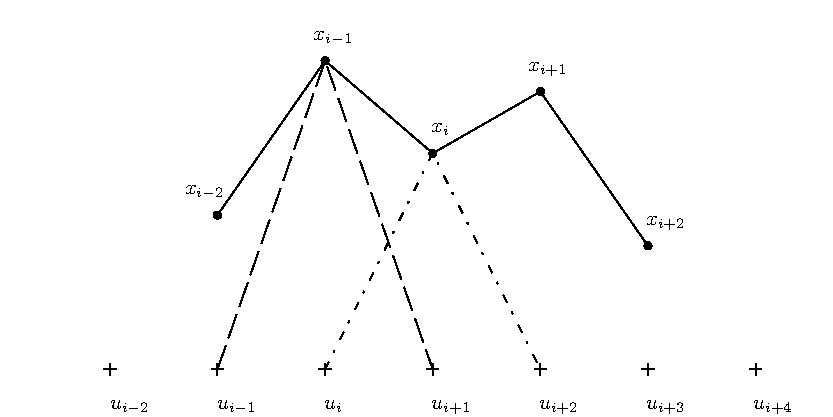
\psfig{file="./images/linearBs.ps",height=6cm,clip=}}
 \caption[B-spline lineari]
  {Esempio di interpolazione con B-splines lineari in cui sono tratteggiate due basi.}
 \lb{Bslin}
\end{figure}

Per comprendere il significato e le propriet\a dei control points e delle basi \e conveniente
considerare dapprima il caso di $d=2$, il pi\u semplice rispetto alle condizioni di
regolarit\a fissate, che corrisponde alle {\it B-splines lineari} (Figura \r{Bslin}).
Il risultato \e l'interpolazione lineare degli stessi punti di controllo $x_i$ dove le basi
$B_i$ sono definite su un intervallo di ampiezza pari a $2$ e hanno forma triangolare.
Fissati quindi $m$ punti o vertici di controllo si hanno $m-1$ segmenti di retta le cui 
equazioni sono esprimibili rispetto al parametro $s$
\beqa
x_{i-1}(s) & = & \,(1-s)\,x_{i-2}\,+\,s\,x_{i-1} \lb{segint}\\
x_i(s) & = & \,(1-s)\,x_{i-1}\,+\,s\,x_i \nonumber\\
x_{i+1}(s) & = & \,(1-s)\,x_{i}\,+\,s\,x_{i+1} \nonumber\\ 
x_{i+2}(s) & = & \,(1-s)\,x_{i+1}\,+\,s\,x_{i+2} \nonumber
\eeqa
$$
con \quad s=\frac{u-u_i}{u_{i+1}-u_i} \quad e \quad u\,\in\,[\,u_i,u_{i+1}\,[
$$
per cui ai due estremi per $s=0$ e $s=1$ corrispondono a $x(0)=x_{i-1}$ e $x(1)=x_i$
rispettivamente\footnotemark.

\footnotetext{Si \e valutato $x(1)$ anche se si \e definito $s$ nell'intervallo aperto
superiormente $[\,0,1\,[$; sarebbe possibile considerare l'intervallo chiuso in quanto
le funzioni splines qui definite sono almeno continue. Cos\iac\,facendo invece si mantengono
gli spans distinti senza punti in comune.}

In Figura \r{Bslin} sono stati tracciati i contributi di $x_{i-1}$ e $x_i$ ricavati
dalle equazioni (\r{segint}) dove si vede che ciascun control points interviene nella
definizione dei due spans adiacenti che lo condividono.
Le due funzioni tratteggiate hanno la stessa forma e altezza che varia con la posizione
dei control points che \e possibile pensarle come le basi $B_i$ di altezza unitaria
scalate dai punti di controllo $x_i$.
Ne risulta che modificando la posizione di un solo vertice si hanno delle variazioni
locali della curva complessiva, per cui si parla di {\it controllabilit\a locale}, che
rappresenta una delle propriet\a fondamentali delle splines.

E' possibile allora esprimere l'equazione del segmento o span (\r{segint}) che collega i due
vertici $x_{i-1}$ e $x_i$ come la combinazione lineare di due basi $B_{i-1}$ e $B_i$
\be
x_i(u)\,=\,x_{i-1}\,B_{i-1}(u)+\,x_i\,B_i(u)
\lb{comb}
\ee
l'imitatamente all'intervallo $u_i \leq u \leq u_{i+1}$ in cui \e definito lo span, con
\[
B_i(u)\,=\,\cases{
           {\ds\frac{u-u_i}{u_{i+1}-u_i}} & $u_i \leq u \leq u_{i+1}$ \cr
              &   \cr                                                    
           {\ds\frac{u_{i+2}-u}{u_{i+2}-u_{i+1}}} & $u_{i+1} \leq u \leq u_{i+2}$. \cr}
\]

\vs(5)

Quanto appena visto pu\o essere esteso all'intera funzione $x(u)$ (o $x(s)$ nel caso di
B-splines uniformi) e quindi anche a $y(s)$; per cui l'intera curva ${\bf r}(u,t)$ risulta
\be
{\bf r}(u,t)\,=\,\sum_{i=0}^{N_B-1}\,{\bf x}_i(t)\,B_i(u) \qquad {\bf x}_i=(x_i,y_i)
\lb{curva}
\ee
oppure
\be
{\bf r}(s,t)\,=\,\sum_{i=0}^{N_B-1}\,{\bf x}_i(t)\,B(s-i)
\ee
nel caso di B-splines uniformi dove la base $B_i$ \e ottenuta semplicemente traslando
la base di riferimento $B$.

%=========================================================================================
\section{B-splines cubiche uniformi}

Consideriamo ora il caso delle {\it B-spline cubiche} ovvero splines ottenute dalla combinazione
di funzioni base che sono costituite da tratti di polinomi cubici ($d=4$).
Inoltre si assuma definitivamente l'ipotesi di splines uniformi per cui i nodi o knots
$u_i$ sono equispaziati; in particolare \e possibile considerarli posti a distanza unitaria
e quindi possono essere sostituiti con una sequenza di interi come in Figura (\r{Bscubic}).
Ciascuna base perci\o \e ottenuta come traslazione di una base di riferimento, come
accennato precedentemente.

\begin{figure}[tbp]
 \centerline{
  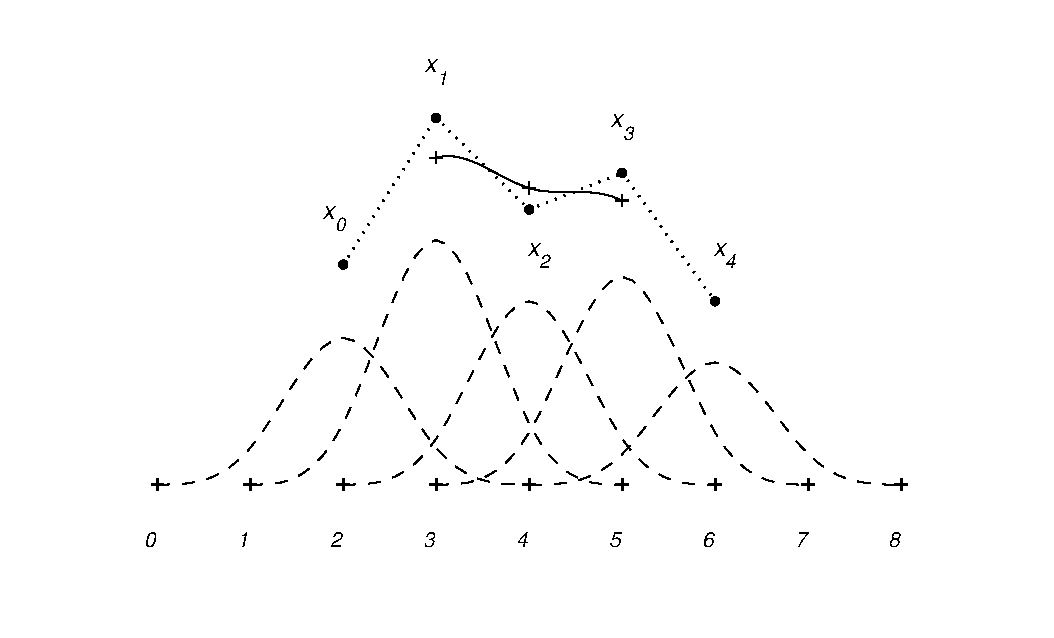
\psfig{file="./images/cubicBs.eps",height=6cm,clip=}}
 \caption[Curva a B-splines cubiche uniformi]
  {Tratto di curva ottenuto dalla combinazione delle funzioni base date dalle B-splines
   cubiche secondo i control points $x_i$. Nel caso di splines uniformi ciacuna base
   $B_i$ \e ottenuta come traslazione di una base di riferimento $B$.}
 \lb{Bscubic}
\end{figure}

A differenza del caso delle B-spline lineari, quelle cubiche non passano
necessariamente per i control points ma al pi\u possono avvicinarsi; tutto dipende dal
numero dei punti di controllo e dalla loro disposizione (nel caso in cui questi siano
allineati la spline deve necessariamente attraversarli).

\begin{figure}[tbp]
 \centerline{
  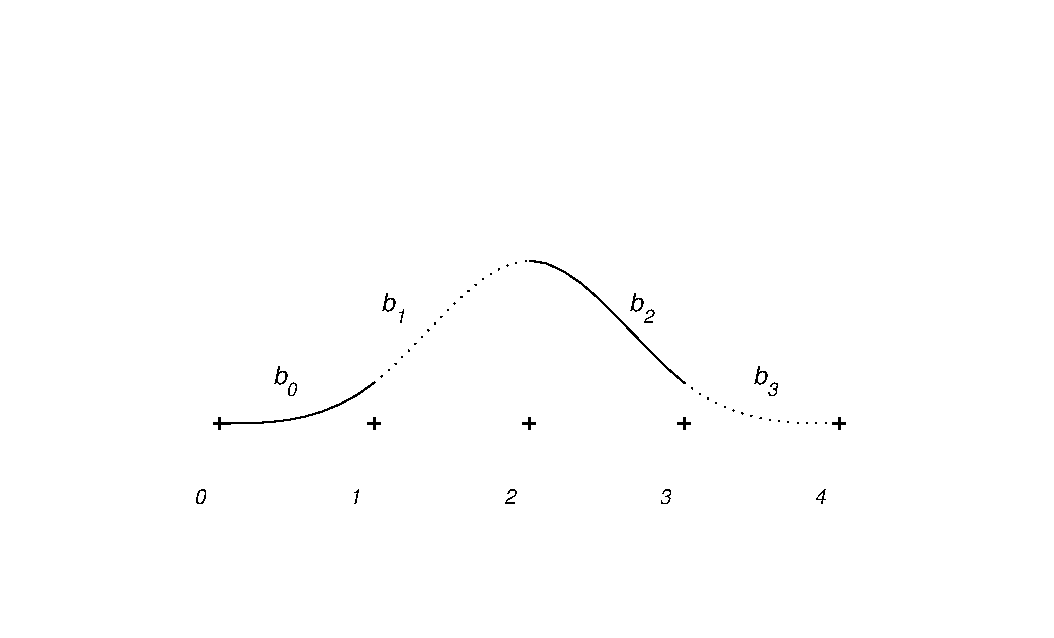
\psfig{file="./images/Bcubic.eps",height=6cm,clip=}}
 \caption[B-spline cubica di riferimento]
  {Base di una B-spline cubica uniforme: \e una curva a tratti di polinomi cubici a supporto
   finito pari a $d=4$ volte la distanza fra due nodi.}
 \lb{BaseBc}
\end{figure}

Dalla Figura \r{Bscubic} si possono individuare alcune caratteristiche della curva ottenuta
dalla combinazione delle B-splines cubiche in particolare, ma che \e possibile estendere
all'intera famiglia delle B-splines:

fissati $m$ {\it control points}, con indice $i=0,\dots,m-1$ 
\ben
\im si hanno $m$ basi $B_i$;
\im la curva \e scomponibile in $m-3$ {\it spans}
\im che si appoggiano su $m-2$ nodi;
\im la spline generata si sviluppa quindi a partire dal quarto nodo $u_3$ e termina in
    corrispondenza del nodo $u_m$.
\een


In Figura \r{BaseBc} \e rappresentata la base $B(s)$ di riferimento menzionata nella
quale sono indicati con diverso tratto i quattro segmenti di polinomio cubico 
\be
a_js^3\,+\,b_js^2\,+\,c_js\,+\,d_j \qquad 0 \leq j \leq 3. 
\ee
Ne risultano quindi $16$ incognite date dai coefficienti dei polinomi che possono essere
individuati in modo univoco considerando i vincoli che derivano dalla regolarit\a imposta
precedentemente alle curve a B-spline, ovvero che siano $C^2$ su tutto il dominio:
\bary(3)
0\,=\,b_0(0)      & 0\,=\,b_0^{(1)}(0)            & 0\,=\,b_0^{(2)}(0)            \\
b_0(1)\,=\,b_1(0) & b_0^{(1)}(1)\,=\,b_1^{(1)}(0) & b_0^{(2)}(1)\,=\,b_1^{(2)}(0) \\
b_1(1)\,=\,b_2(0) & b_1^{(1)}(1)\,=\,b_2^{(1)}(0) & b_1^{(2)}(1)\,=\,b_2^{(2)}(0) \\
b_2(1)\,=\,b_3(0) & b_2^{(1)}(1)\,=\,b_3^{(1)}(0) & b_2^{(2)}(1)\,=\,b_3^{(2)}(0) \\
b_3(1)\,=\,0      & b_3^{(1)}(1)\,=\,0            & b_3^{(2)}(1)\,=\,0            
\eary
che come si nota impongono la continuit\a fino alla derivata seconda ($d-2$) compresa nei
punti di raccordo o {\it breakpoints} tra le curve polinomiali valutati per $s=0$ e $s=1$.

Un'ultima condizione \e fissata imponendo che
$$
b_0(0)\,+\,b_1(0)\,+\,b_2(0)\,+\,b_3(0)\,=\,1
$$
che si riduce a 
$$
b_1(0)\,+\,b_2(0)\,+\,b_3(0)\,=\,1
$$
dato che \e gi\a stato fissato $b_0(0)=0$.

Risolvendo le equazioni nei coefficienti incogniti $a_j$, $b_j$, $c_j$, $d_j$ per i quattro
segmenti che compongono $B$ si ricava
\beqa
b_0(s) & = & \frac{1}{6}\,s^3 \nonumber\\
 & \nonumber\\
b_1(s) & = & \frac{1}{6}\,\Big(\,-3s^3+3s^2+3s+1\,\Big) \nonumber\\
 & \lb{polcubic}\\
b_2(s) & = & \frac{1}{6}\,\Big(\,3s^3-6s^2+4\,\Big) \nonumber\\
 & \nonumber\\
b_3(s) & = & \frac{1}{6}\,\Big(\,-s^3+3s^2-3s+1\,\Big) \nonumber
\eeqa

Da queste \e possibile ottenere un'interessante espressione per lo {\it span} $i-esimo$ definito
sull'intervallo $[u_i,u_{i+1}[$.
A partire dalla (\r{curva}), trascurando per semplicit\a la variabile temporale,
\be
{\bf r}(u)\,=\,\sum_{i=0}^{N_B-1}\,{\bf x}_i\,B_i(u);
\ee
e tenendo presente che la base $B_i$ e non nulla solo su $[u_i,u_{i+d}[$, allora nell'inter-vallo
$[u_i,u_{i+1}[$ intervengono solo un numero finito, pari a $d$, di basi 
\beqa
{\bf r}_i(u) & = & \sum_{j=0}^{3}\,{\bf x}_{i-j}\,B_{i-j}(u)\,= \nonumber\\
             &   & \\
             & = & {\bf x}_{i}\,B_{i}(u)\,+\,{\bf x}_{i-1}\,B_{i-1}(u)\,+\,
                   {\bf x}_{i-2}\,B_{i-2}(u)\,+\,{\bf x}_{i-3}\,B_{i-3}(u) \nonumber
\eeqa

Inoltre, limitatamente all'intervallo considerato, la $B_i$ contribuisce con il tratto di
polinomio $b_i$ per cui l'espressione si semplifica ulteriormente nella
\beqa
{\bf r}_i(s) & = & \sum_{j=0}^{3}\,{\bf x}_{i-j}\,b_{j}(s)\,= \nonumber\\
             &   & \lb{rsempl}\\
             & = & {\bf x}_{i}\,b_{0}(s)\,+\,{\bf x}_{i-1}\,b_{1}(s)\,+\,
                   {\bf x}_{i-2}\,b_{2}(s)\,+\,{\bf x}_{i-3}\,b_{3}(s) \nonumber
\eeqa
per ogni quaterna $[\,{\bf x}_i,{\bf x}_{i-1},{\bf x}_{i-2},{\bf x}_{i-3}\,]$ di
{\it control points}.

\boss
Il vantaggio di quest'ultima espressione \e che pu\o essere convenientemente espressa in
forma matriciale.
Riordinando i termini della (\r{rsempl}) nella forma
\be
{\bf r}_i(s)\,=\,{\bf x}_{i-3}\,b_{3}(s)\,+\,{\bf x}_{i-2}\,b_{2}(s)\,+\,
                 {\bf x}_{i-1}\,b_{1}(s)\,+\,{\bf x}_{i}\,b_{0}(s) 
\ee
la si pu\o scrivere come prodotto di vettori
\be
{\bf r}_i(s)\,=\,{\bf b}(s)\,{\bf x}_i\,=\,
                 \qmatrix{b_3(s) & b_2(s) & b_1(s) & b_0(s)\cr}\,
                 \qmatrix{{\bf x}_{i-3} \cr
                          {\bf x}_{i-2} \cr
                          {\bf x}_{i-1} \cr
                          {\bf x}_{i} \cr}.
\ee
Espandendo i termini $b_j$ il primo vettore risulta
\be
{\bf b}(s)\,=\,{\bf s}^T\,{\bf M}\,=\,\frac{1}{6}
               \qmatrix{s^3 & s^2 & s & 1 \cr}\,
               \smatrix{4}{ -1 &  3 & -3 &  1 \cr
                             3 & -6 &  3 &  0 \cr
                            -3 &  0 &  3 &  0 \cr
                             1 &  4 &  1 &  0 \cr} 
\ee   
e quindi concludendo

\be
{\bf r}_i(s)\,=\,\frac{1}{6}\,{\bf s}^T\,{\bf M}\,{\bf x}_i
\lb{cBsmat}
\ee
\eoss

\begin{figure}[tbp]
 \centerline{
  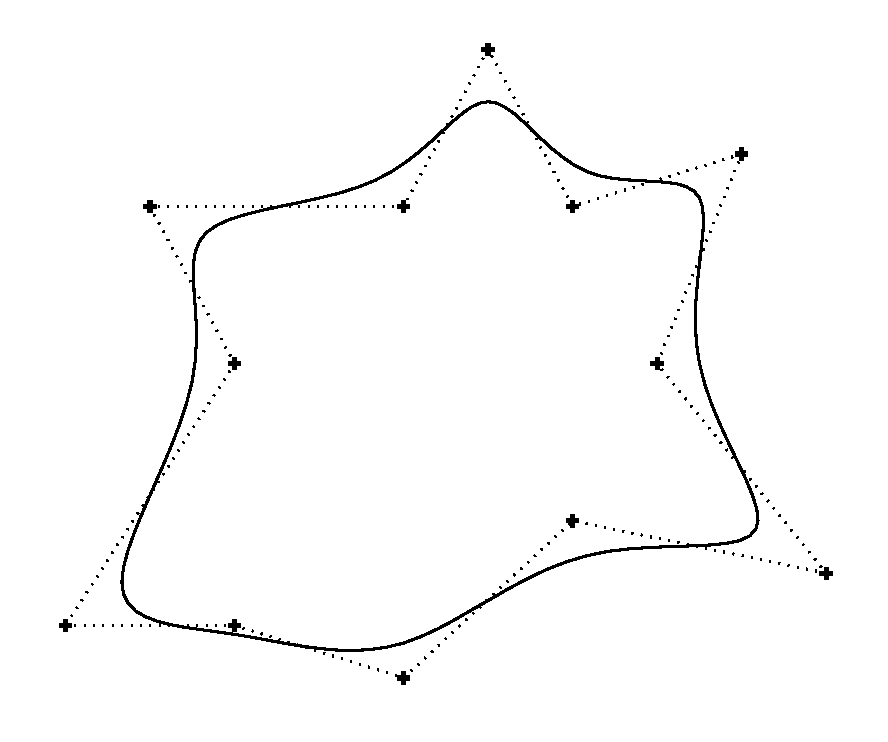
\psfig{file="./images/conv_h1.eps",height=6cm,clip=}}
 \caption[Curva 2D a B-splines ]
  {Esempio di curva bidimensionale chiusa a B-splines cubiche uniformi con poligono dei
   control points.}
 \lb{curva2d}
\end{figure}

%=======================================================================================
\section{Alcune propriet\a delle B-splines}

%---------------------------------------------------------------------------------------
\subsection{Convex hull}

\begin{figure}[tbp]
 \centerline{
  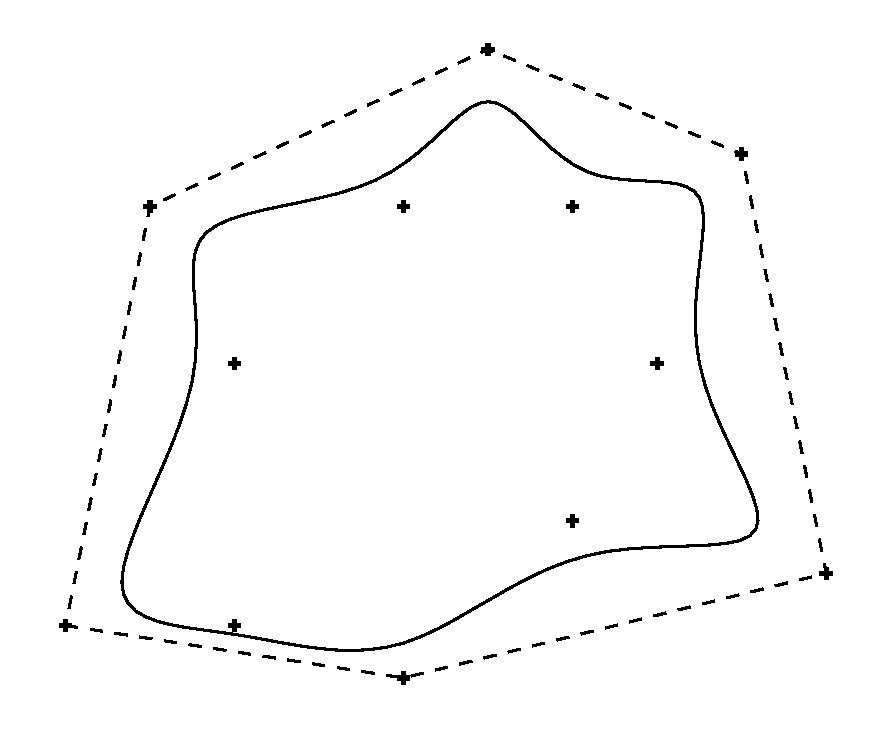
\psfig{file="./images/conv_h2.eps",height=6cm,clip=}}
 \caption[Convex Hull]
  {La regione convessa, convex hull, che contiene tutti i control points e la curva di 
   figura (\r{curva2d}).}
 \lb{convhull}
\end{figure}

In figura (\r{convhull}) \e rappresentato la {\it convex hull} dell'insieme $Q$ dei
{\it control points} definita come il pi\u piccolo poligono convesso tale per cui tutti 
i punti di $Q$ o sono interni o al pi\u appartengono al bordo.

\vs(5)

Dalla definizione di insieme convesso
\bdf
{\bf Insieme convesso.}\par
Si dice che un sottoinsieme $A$ di uno spazio vettoriale \e convesso quando verifica la
condizione:
\be
\alpha\,{\bf x}_1\,+\,(1-\alpha)\,({\bf x}_2-{\bf x}_1)\,\in\,A \qquad 
 \forall\,{\bf x}_1,{\bf x}_2\in A \quad \forall\,\alpha\in [0,1]
\ee
\edf
(Nel nostro caso lo spazio considerato \e $\M(R)^2$ e l'insieme $A$ \e la convex hull).

\e possibile ricavare la condizione che caratterizza la convex hull in funzione dei
control points, ovvero
\bpr
\par
Ciascun punto {\bf p} della convex hull pu\o essere espresso come combinazione lineare
convessa dei control points $[{\bf x}_0,\dots,{\bf x}_{m-1}]$
\be
{\bf p}\,=\,\sum_{i=0}^{m-1}\,w_i\,{\bf x}_i\, ,\qquad
w_i \geq 0\quad\forall i \quad e \quad \sum_{i=0}^{m-1}\,w_i\,=\,1
\ee
\epr   

Si consideri lo span definito dai control points $[{\bf x}_0,{\bf x}_1,{\bf x}_2,{\bf x}_3]$
di Figura \r{Bscubic}; questi risulta contenuto nella convex hull definita dai suoi
$4$ control points nell'ordine, antiorario, $\{{\bf x}_0,{\bf x}_2,{\bf x}_3,{\bf x}_1\}$.
Infatti vale la proposizione precedente in quanto si verifica dalle (\r{polcubic}) che
\be
\sum_{j=0}^{3}\,b_j(s)\,=1 \qquad \forall\quad s \in \,[0,1[
\lb{sumunit}
\ee
ed inoltre $b_j(s)$ \e non negativa, quindi i nostri $w_i$ sono proprio i $b_j$.

In base a questi risultati, noto il poligono dei control points, \e possibile conoscere
lo spazio in cui si trova la curva a B-splines.
In particolare la B-spline approssima in modo regolare le variazioni del poligono
dei control points.

%---------------------------------------------------------------------------------------
\subsection{Invarianza alle traslazioni}

Con tale propriet\a si vuole indicare che anche se i {\it control points} ${\bf x}_i$ vengono
traslati della stessa quntit\a ${\bf v}$ la nuova curva descritta ${\bf r_v}$ \e ottenuta
applicando la stessa traslazione a tutti i punti della curva originaria ${\bf r}$.

\be
{\bf r_v}(u)\,=\,\sum_{i=0}^{m-1}\,B_i(u)\,({\bf x}_i+{\bf v})\,=\,
                 \sum_{i=0}^{m-1}\,B_i(u)\,{\bf x}_i\,+\,
                 {\bf v}\,\sum_{i=0}^{m-1}\,B_i(u)            
\ee

Per la propriet\a precedente (\r{sumunit}) la seconda sommatoria \e pari a $1$ per cui risulta
\be
{\bf r_v}(u)\,=\,\sum_{i=0}^{m-1}\,B_i(u)\,{\bf x}_i\,+\,{\bf v}\,=\,
                 {\bf r}(u)\,+\,{\bf v} \qquad \forall\, u
\ee

%---------------------------------------------------------------------------------------
\subsection{Invarianza alle rotazioni e alle omotetie}

\begin{figure}[tbp]
 \centerline{
  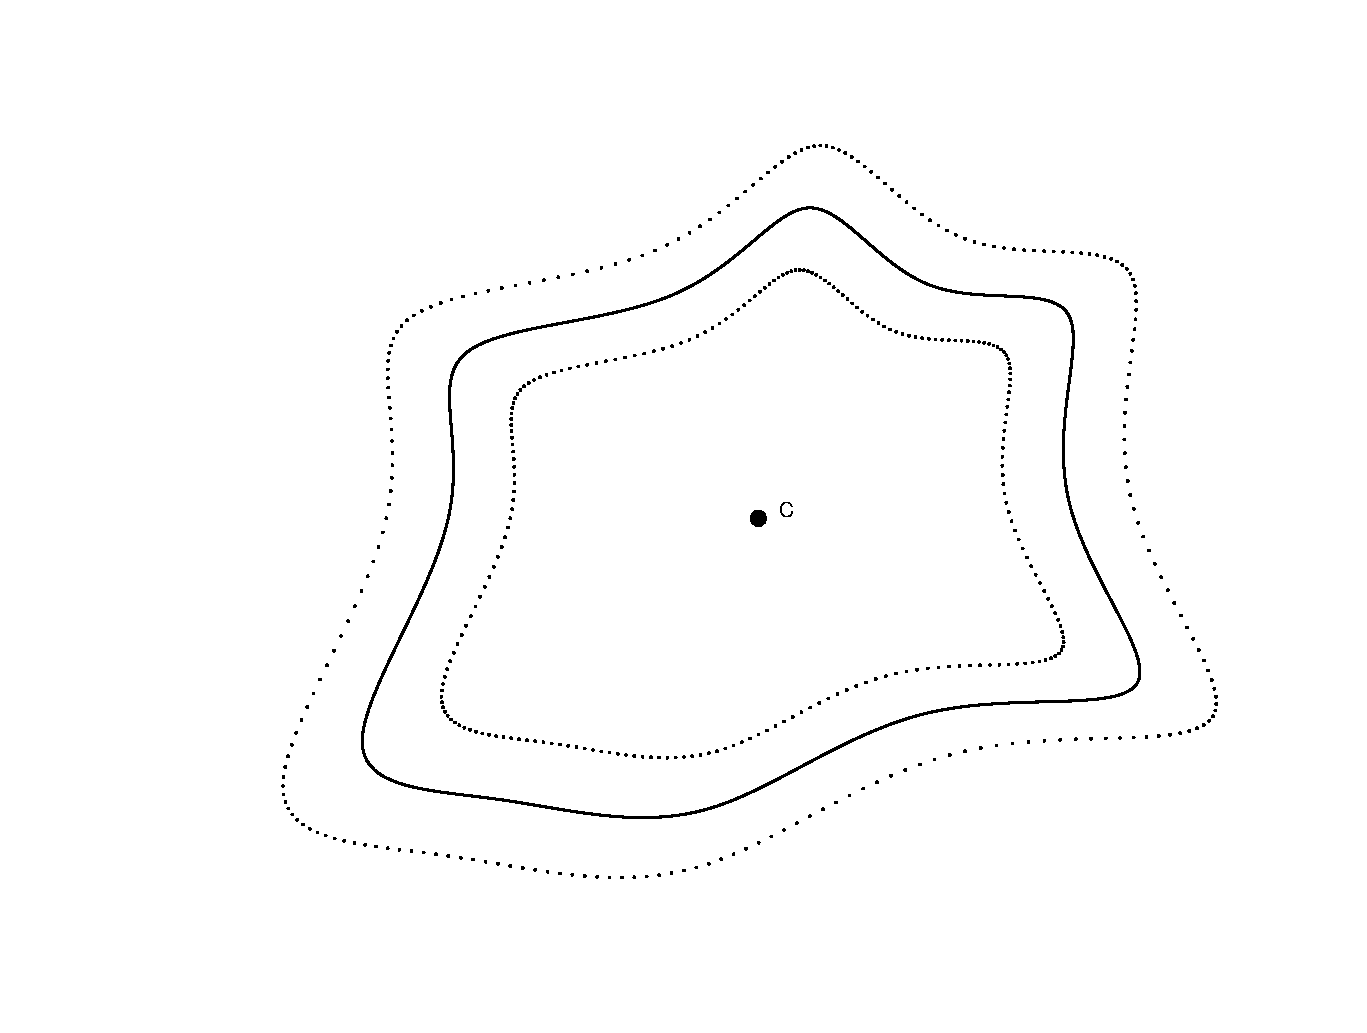
\psfig{file="./images/omotetia.eps",height=6cm,clip=}}
 \caption[Omotetia rispetto al centroide dei control points]
  {Due casi di omotetia rispetto al centroide ${\bf c}$ dei {\it control points}: una
   {\it dilatazione} e una {\it contrazione}}
 \lb{omotetia}
\end{figure}

E' possibile verificare la stessa invarianza sia per le rotazioni sia per le omotetie 
(dilatazioni o contrazioni).

\bi
\im {\it Rotazione}. La rotazione di un angolo $\theta$  
    \be
    {\bf R}(\theta)\,=\,\smatrix{2}{ \cos\theta & -\sin\theta \cr
                                     \sin\theta &  \cos\theta \cr}
    \ee
    \be
    {\bf r_{R(\theta)}}(u)\,=\,\sum_{i=0}^{m-1}\,B_i(u)\,{\bf R(\theta)}{\bf x}_i\,=\,
                               {\bf R(\theta)}\,\sum_{i=0}^{m-1}\,B_i(u)\,{\bf x}_i\,=\,
                               {\bf R(\theta)}\,{\bf r}(u)            
    \ee

\im {\it Omotetie}. Si considera in particolare il cambiamento di scala di fattore $\gamma$ 
    definito rispetto al centroide ${\bf c}$ dei punti di controllo come in Figura \r{omotetia}
    \beqa
    {\bf r_{\bf c}}(u) & = & \sum_{i=0}^{m-1}\,B_i(u)\,[\gamma\,({\bf x}_i-{\bf c})+{\bf c}] \nonumber\\
                       & = & \gamma\,\sum_{i=0}^{m-1}\,B_i(u)\,{\bf x}_i\,+\,
                             (1-\gamma)\,{\bf c}\,\sum_{i=0}^{m-1}\,B_i(u)\,= \nonumber\\
                       & = & \gamma\,{\bf r}(u)\,+\,(1-\gamma)\,{\bf c}
    \eeqa
    in quanto la seconda sommatoria \e pari a $1$ per la propriet\a di {\it convex hull}
    definita precedentemente, e dove
    \be
    {\bf c}\,=\,\frac{1}{N}\,\sum_{i=0}^{m-1}\,{\bf x}_i
    \ee
    La trasformazione esposta pu\o essere espressa in una forma pi\u compatta come
    prodotto di matrici (a tal proposito si veda l'Appendice \r{A2}).
\ei   

%=======================================================================================
\section{Condizioni per gli estremi delle curve a B-splines}

Considerando la Figura \r{Bscubic} si pu\o notare che gli estremi della curva, composta
di due spans, non sono vincolati a dei punti particolari, ma le loro coordinate sono
comunque note valutando la (\r{rsempl}) per $s=0$ e $s=1$ con le rispettive quaterne di
control points.
In generale quindi se $[{\bf x}_0,\dots,{\bf x}_{m-1}]$ \e il vettore dei control points
le coordinate dei punti di "inizio" ${\bf p}_s$ e di "fine" ${\bf p}_e$ della curva risultano
\beqa
{\bf p}_s & = & {\bf r}_3(0)\,=\,\frac{1}{6}\,\bigg[{\bf x}_0+4{\bf x}_1+{\bf x}_2\bigg]
                \nonumber\\
          &   & \\
{\bf p}_e & = & {\bf r}_{m-1}(1)\,=\,\frac{1}{6}\,\bigg[{\bf x}_{m-3}+4{\bf x}_{m-2}+
                                                        {\bf x}_{m-1}\bigg] \nonumber
\eeqa

Per ottenere un comportamento diverso per gli estremi, quale pu\o essere la condizione che li
vuole coincidenti con il primo e l'ultimo control points, si pu\o procedere in due modi:
\bi
\im nel caso particolare delle B-splines uniformi si realizzano i {\it multiple vertices}
    ottenuti raddoppiando o triplicando i due vertici estremi; oppure inserendo altri punti
    di controllo noti come {\it phantom vertices} (\cite{Bartels})
\im un'altra soluzione \e quella di prevedere per gli estremi delle basi differenti (si parla
    in tal caso di B-splines {\it aperiodiche}) ottenute moltiplicando i {\it nodi} e non
    i punti di controllo. In questo modo si riducono i vincoli sulla regolarit\a della base
    e quindi \e possibile utilizzare i gradi di liber-t\a in pi\u per condizionare la posizione
    degli estremi, senza introdurre altri control points (\cite{BlakeAC}).
\ei

%------------------------------------------------------------------------------------------
\subsection{Curve a B-splines chiuse}

Un caso particolarmente interessante per l'applicazione considerata in queta tesi \e dato
dalle a curve a B-splines chiuse, ovvero in cui i due punti ${\bf p}_s$ e ${\bf p}_e$
coincidono (si veda la Figura \r{curva2d}).
E' realizzata semplicemente ponendo uguali i primi e gli ultimi $3$ {\it control points},
ovvero assegnato il vettore ${\bf X}=[{\bf x}_0,\dots,{\bf x}_{m-1}]$ si considera il nuovo
vettore $\hat{\bf X}=[{\bf x}_0,\dots,{\bf x}_{m-1},{\bf x}_0,{\bf x}_1,{\bf x}_2,]$.

%=======================================================================================
\section{Punti singolari delle curve a B-splines}\lb{PSCBS}

Le osservazioni fatte precedentemente sui vincoli per gli estremi delle curve a B-spline
valgono anche nel momento in cui si conceda che la curva abbia delle singolarit\a nelle
derivate, per cui non risulta pi\u $C^{(d-2)}$, come nel caso tipico di punti angolosi o
{\it hinge}.

Nel caso delle B-spline uniformi ci\o pu\o essere ottenuto in due modi:
con l'inserimento di control points interni multipli\footnotemark, oppure, pi\u opportunamente,
introducendo la singolarit\a nelle basi delle B-splines. 

\footnotetext{Aumentare il numero di control points in un tratto della curva significa
anche aumentare il rischio che la curva possa assumere conformazioni non volute come
ad esempio cappi.}

\vs(5)

Per ulteriori considerazioni si rimanda ai riferimenti \cite{BlakeAC}, \cite{Bartels}
in cui \e possibile trovare anche gli algoritmi per il calcolo ricorsivo delle basi
nel caso pi\u generale.

\finepar


% Contorni Attivi
\chapter{Contorni attivi}\lb{CA}

Nel Capitolo \r{SGM} si \e accennato all'utilizzo di alcuni operatori locali che permettono di
individuare nell'immagine delle opportune primitive ({\it features}) il cui insieme costituisce una nuova
immagine o mappa delle primitive ({\it features map}) la cui interpretazione pu\o permettere di
individuare gli elementi (oggetti) che compongono l'immagine.

Il problema \e che, tranne in casi molto fortunati in cui si hanno immagini costituite da
elementi distinti, prive di particolari disturbi e con superfici dei materiali ripresi sostanzialmente uniformi,
vi possono essere diverse false {\it features}.
Occorre pertanto definire un criterio che permetta di estrarre solo quelle vere.
Nel caso pi\u semplice si pu\o considerare una funzione costante che coincide con un
valore di soglia, valore che per\o pu\o non essere semplice individuare e che inoltre pu\o generare
il problema opposto, ovvero portare ad eliminare anche alcune {\it features} buone che per\o
sono "deboli", per cui si ottiene una descrizione frammentaria della {\it features map} 
dell'immagine che ne complica la successiva elaborazione.

Come gi\a accennato precedentemente, una soluzione di notevole interesse 
\e data dagli {\it active contours}, chiamati comunemente {\it snakes}\footnotemark \cite{Kass}.

\footnotetext{La famiglia degli {\it active contours} \e costituita oltre che da {\it snakes},
che ne solo la forma pi\u semplice, anche da {\it deformable template} e {\it dynamic contours}\cite{BlakeAC}}.


%======================================================================================
\section{Snakes}

Con {\it snake} si intende una curva deformabile ${\bf r}(s)$, $0 \leq s \leq 1$,
che sotto l'azione di opportune "forze" definite nello spazio delle primitive 
dell'immagine tende a deformarsi in modo da minimizzare una "energia" o
"funzione costo".
Nel caso particolare della soluzione di problemi di segmentazione tale funzione
\e definita in modo che la condizione di minimo porti la curva ad adagiarsi lungo
i contorni degli oggetti, per cui lo spazio delle primitive \e dato generalmente dalla 
mappa degli {\it edgles}.

\boss
Determinare la mappa delle features completa pu\o richiedere tempi eccessivi per
l'applicazione considereta, ed inoltre non \e detto sia necessario; per cui tali
primitive possono essere individuate limitatamente all'intorno della curva analizzando
l'immagine lungo direzioni particolari, tipicamente lungo la normale alla curva
\cite{BlakeAC}.
\lb{ossploc}
\eoss

L'energia totale ${\cal E}({\bf r})$, lungo tutta la curva, che individua lo stato dello
snake \e composta di due termini
\be
{\cal E}({\bf r})\,=\,{\cal E}_s({\bf r})\,+\,{\cal P}({\bf r}).
\lb{ergtot}
\ee
\ben
\im
Il primo rappresenta l'{\it energia interna} che controlla la regolarit\a della curva
e quindi un vincolo sulla classe delle forme che pu\o segmentare:
\be
{\cal E}_s({\bf r})\,=\,\int_0^1\,w_1(s)|{\bf r}_s|^2\,+
                                \,w_2(s)|{\bf r}_{ss}|^2\,ds,\quad (\footnotemark)
\ee 

\footnotetext{Con $f_x$ si denota la derivata di $f$ rispetto alla variabile $x$.}

dove $w_1(s)$ controlla l'"elasticit\a" rispetto alle sollecitazioni che tendono a dilatare
o comprimere lo snake (trazione e compressione) e $w_2(s)$ la "rigidezza" rispetto alle 
deformazioni trasversali allo snake (flessione).

Infatti se si aumentasse solo $w_1(s)$, minimizzare l'energia corrisponderebbe ad accorciare
la lunghezza della curva fino, caso limite, a ridurla ad un punto; nel caso di $w_2(s)$
invece si avrebbe la tendenza ad aumentare la regolarit\a della curva fino ad approssimare
una linea retta. Al contrario riducendo i due termini, al limite ponendoli a zero\footnotemark,
\e possibile ottenere una curva che presenti dei punti angolosi o addidrittura delle
discontinuit\a.

\footnotetext{I coefficienti $w_1(s)$ e $w_2(s)$ sono non negativi.}

\im
Il secondo termine della (\r{ergtot}) rappresenta l'{\it energia potenziale} dello {\it snake}
rispetto allo spazio delle primitive; per cui se $\cal P$ \e definita in modo tale
che i suoi punti di minimo siano in corrispondenza delle {\it features}, allora la minimizzazione
della (\r{ergtot}) spinge lo snake ad approssimarle.
L'energia potenziale lungo tutta la curva pu\o essere definita come l'integrale curvilineo
di una funzione potenziale 
\be
{\cal P}({\bf r})\,=\,\int_0^1\,P({\bf r}(s))\,ds
\ee
dove $P({\bf r})$ \e una funzione che mappa i punti dell'immagine nello spazio delle primitive.
Alcuni esempi tipici delle definizioni di $P({\bf r})$ sono
 \ben
 \im $P({\bf r})\,=\,\pm\,c\,\bigg(\,G_\sigma \ast I\,({\bf r})\,\bigg)$
     se si considera come primitiva i picchi di intensit\aac: bassa o alta intensit\aac, chiaro o
     scuro, a seconda del segno;
 \im $P({\bf r})\,=\,-\,c\,\Big|\,\nabla\bigg(\,G_\sigma \ast I\,({\bf r})\,\bigg)\,\Big|$
     in questo caso si considerano gli {\it edgels}.
 \een
Per entrambi i casi si sono considerati solo i punti della curva, ${\bf r}(s)$, in base
all'osservazione \r{ossploc}.

Come accennato nel caso degli {\it edge-detector}, l'azione della convoluzione con la gaussiana 
$G_\sigma(x,y)$ \e rivolto sia alla riduzione dell'$SNR$ all'uscita del filtro $P(x,y)$
sia a migliorare il grado di localizzazione degli {\it edgels}.
Nel caso degli {\it snakes} questo pu\o essere visto come una trasformazione della superficie
su cui esso si muove, l'immagine, che possa da un lato facilitare l'avvicinamento ai punti
del contorno ($\sigma$ grande) e dall'altro fare in modo che l'errore di approssimazione
ammesso (in termini di localizzazione del bordo) sia piccolo ($\sigma$ piccola).
Anche in questo caso le due condizioni lavorano in direzioni opposte, per cui
risulta non sempre facile fissare un valore per tutte le zone dell'immagine;
eventualmente si potrebbe considerare $\sigma$ variabile in base alle caratteristiche
locali dell'immagine stessa come nel caso degli operatori anisotropi.
\een

%-------------------------------------------------------------------------------------
\section{Un approccio Lagrangiano}

La soluzione al problema della minimizzazione dell'energia $\cal E$ pu\o essere determinata
in modo statico calcolando direttamente i punti di estremo; in realt\aac, anche in considerazione
del modo in cui vengono determinate le primitive, \e conveniente considerare lo {\it snake}
come una curva che si muove sul piano immagine ({\it dynamic snake}) la cui posizione e forma
variano ad ogni passo in relazione alle misure effettuate; ne deriva che la 
condizione di minimo dell'energia coincide perci\o con lo stato di equilibrio del sistema
dinamico.

Il nuovo modello \e ottenuto ridefinendo la carta ${\bf r}(s,t)$ per tener conto della 
variazione nel tempo $t$ e considerando che la curva abbia una densit\a di massa $\mu (s)$,
per cui \e presente anche una componente di energia cinetica
\be
{\cal T}({\bf r})\,=\,\frac{1}{2}\int_0^1\,\mu (s)|{\bf r}_t|^2\,ds
\ee
A causa dell'inerzia introdotta da $\mu (s)$, affinch\'e il sistema raggiunga uno stato
stabile \e necessario introdurre un termine a cui sia affidata la dissipazione dell'energia
cinetica immagazzinata.
A tal scopo si pu\o considerare la funzione {\it dissipazione di Rayleigh} definita
\be
{\cal D}({\bf r}_t)\,=\,\frac{1}{2}\int_0^1\,\gamma |{\bf r}_t|^2\,ds.
\ee
Applicando il {\it principio di Hamilton} si perviene alle {\it equazioni di Lagrange}
\cite{BlakeAV1}
\be
\mu {\bf r}_{tt}\,+\,\gamma {\bf r}_t\,-\,\frac{\partial}{\partial s}\,(w_1{\bf r}_s)\,+
 \,\frac{\partial^2}{\partial s^2}\,(w_2{\bf r}_{ss})\,=\,-\nabla P({\bf r}(s,t))
\lb{eqlagr}
\ee
in cui si sono considerate $\mu (s)=\mu$ e $\gamma (s)=\gamma$ costanti lungo tutta
la curva.
     
%....................................................................................
\subsubsection{Kalman-snakes}

Tenendo conto della dinamica dello snake \e possibile risolvere problemi pi\u complessi
in cui la mappa delle {\it features} varia nel tempo a cusa del moto relativo tra il sensore
e l'oggetto da inseguire: si parla perci\o di {\it data tracking}.
In questo caso l'equilibrio raggiunto \e dinamico in quanto lo snake tende ad approssimare
dei dati che non sono costanti nel tempo.
Le prestazioni del sistema migliorano sensibilmente se si integrano nel tempo le misure
delle primitive con il modello dinamico dello snake utilizzando il {\it filtro di Kalman},
il cui passo di predizione permette di stabilire come potr\a essere l'evoluzione dello
snake al passo successivo individuando la regione di confidenza entro cui sar\a probabile
trovarlo nell'immagine succesiva.
La posizione reale verr\a individuata dalle misure effettuate nel passo di aggiornamento.

L'introduzione del filtro, il cui peso computazionale \e generalmente trascurabile,
permette di ridurre la regione dell'immagine su cui effettuare le misure, che \e la
componente critica per la quantit\a di dati considerati, e quindi migliorare l'efficienza
generale dell'algoritmo.

%---------------------------------------------------------------------------------------
\section{Contorni dinamici}

Nel modello utilizzato finora gli unici vincoli sulle deformazioni a cui \e soggetto lo snake
sono dati dai termini di energia interna associati ai coefficienti $w_1(s)$ e $w_2(s)$.

Esiste la possibilit\a di vincolare la curva in modo che assuma delle forme che si discostino
relativamente da un modello prefissato ({\it template}).
La curva \e quindi definita da una carta ${\bf r}(s;{\bf X})$ \cite{BlakeAC}
che \e funzione di un vettore di parametri che tengono
conto delle possibili trasformazioni che questa pu\o subire (rotazioni, traslazioni,
dilatazioni, etc.); ovvero a partire da una forma di
riferimento si applicano le trasformazioni, scelte fra quelle accettabili, che permettono 
di sovrapporla all'oggetto corrispondente che si trova sul piano immagine:
si parla perci\o di {\it deformable templates}.

Considerando quindi il modello dinamico definito dai {\it Kalman snakes} proiettato
nello spazio delle forme ({\it deformable templates}) si ottengono i {\bf contorni dinamici}
o {\bf dynamic contours}.

%========================================================================================
\section{Discretizzazione dello snake}

Le soluzioni dell'equazione (\r{eqlagr}) sono curve continue nello spazio $\M(R)^2$, mentre
per poterle elaborare numericamente \e necessario discretizzarle.
Il modo pi\u semplice \e dato dal campionamento della curva con un passo di campionamento
$h=1/(N-1)$ nello spazio del parametro $s\in[0,1]$ per cui i campioni della curva sono 
${\bf r}(i\,h)$ con $i=1,\dots,N$.
L'equazione differenziale si trasforma perci\o in un'equazione alle differenze sostituendo
le derivate prima e seconda con le espressioni \footnotemark
\be
{\bf r}_s(s_i)\,=\,\frac{{\bf r}(s_i)\,-\,{\bf r}(s_{i-1})}{h} \quad e \quad
{\bf r}_{ss}(s_i)\,=\,\frac{{\bf r}(s_{i+1})\,-2\,{\bf r}(s_i)\,+\,{\bf r}(s_{i-1})}{h^2}
\ee
Analogamente per le derivate rispetto la variabile temporale $t$.

\footnotetext{Discretizzazione con metodo di Eulero implicito.}

L'equazione di Lagrange (\r{eqlagr}) viene espressa da una equazione differenziale
del secondo ordine \cite{BlakeAV1}
\be
{\bf M\,\ddot{u}}\,+\,{\bf C\,\dot{u}}\,+\,{\bf K\,u}\,=\,{\bf f} \quad con \quad
{\bf u}=\{{\bf u}_i\}_{i=1,\dots,N}={\bf r}(i\,h)
\ee
dove ${\bf M}$ \e la matrice delle masse, ${\bf C}$ tiene conto dei fenomeni di dissipazione,
${\bf K}$ della rigidezza dello snake e ${\bf f}$ dipende da $\nabla P$.

Effetto del campionamento della curva \e la perdita della propriet\a di continuit\a 
e quindi dell'informazione sulla forma individuata dallo {\it snake} stesso, per cui,
sia nel caso particolarmente interessante dei contorni dinamici accennati precedentemente
sia nel caso dei semplici {\it snake} nella forma data dall'equazione (\r{ergtot}), si ricorre
ad approssimazioni con metodi agli "{\it elementi finiti}" in cui la curva ${\bf r}$ \e
definita dalla combinazione lineare di particolari funzioni $B_i$, elementi della base di un
opportuno spazio vettoriale, pesate dai {\it nodi} ${\bf q_i}(t)$
\be
{\bf r}(s,t)\,=\,\sum_{i=1}^N\,B_i(s)\,{\bf q}_i(t)
\ee
Un modello particolarmente interessante, che sar\a considerato nel nostro caso, \e dato
dall'approssimazione a {\bf splines} in cui la curva \e approssimata da funzioni polinomiali
a tratti parametrizzate dai nodi ${\bf q_i}(t)$ che prendono il nome di {\it control points} \cite{BlakeAV2} \footnotemark. 

\footnotetext{Altre descrizioni parametriche del contorno possono essere ricavate utilizzando i coefficienti
di Fourier.}

%========================================================================================
\section{Un approccio statistico}

L'introduzione degli {\it snakes} ha permesso di risolvere alcuni problemi che affliggono i metodi
di segmentazione che si basano sulla sola {\it edge-detection} fornendo un modello che permette
di mantenere le informazioni sulla forma degli oggetti a cui appartengono gli {\it edgels}.

Si \e quindi posto il problema come la minimizzazione di una particolare funzione
energia, dove il termine legato all'immagine \e definito da un potenziale, che \e minimo
in corrispondenza dei bordi dei segmenti.

Finora si \e considerato il potenziale definito in funzione delle propriet\a locali 
nell'intorno della curva ({\it feautures}) e in particolare considerando il gradiente dell'immagine
opportunamente filtrata; ma, a causa dell'operatore differenziale, 
tali misure sono molto sensibili ai disturbi di diversa natura
che possono essere presenti nell'immagine stessa, ovvero
tale sensibilit\a pu\o essere ridotta con un aumento
dell'azione filtrante ma a scapito della capacit\a di localizzazione.

Per ovviare a tale limite sono state proposte soluzioni alternative che 
tengono conto anche delle propriet\a di omogeneita dei segmenti.
Si possono individuare due strade:
\ben
\im si identificano i bordi in modo indiretto, senza utilizzare operatori differenziali,
    ridefinendo un'opportuna energia che tenga conto anche della statistica dei segmenti
    e forzando i contorni attivi a disporsi in modo da massimizzare la differenza fra
    i segmenti separati dai contorni stessi \cite{Yezzi}, \cite{Yuille};
\im considerando i due approcci distinti che interagiscono fra di loro in base ad opportune
    regole \cite{Duncan} che stabiliscono come il risultato di uno venga valutato
    dall'altro e quindi la possibile contromossa pi\u conveniente in termini di "costo",
    fino a giungere ad una condizione di equilibrio.
\een

%---------------------------------------------------------------------------------------
\subsection{L'algoritmo di Yezzi, Tsai e Willsky}\lb{AYTW}

Nell'ambito delle soluzioni del primo tipo vi \e l'algoritmo proposto da A. Yezzi, A. Tsai
e A. Willsky in \cite{Yezzi} che permette di incorporare in un nuovo modello di {\it snake}
sia informazioni locali sia globali attraverso una funzione energia diversa da quelle
considerate finora.
Il vincolo principale nell'utilizza-re il modello proposto \e che siano note a priori 
come le primitive scelte per la segmentazione descrivono i diversi elementi dell'insieme
da segmentare, per cui ad ogni oggetto sia associabile un valore per ogni feature.
\boss
Il valore non deve essere necessariamente noto ma ,se esiste, si deve poter dire che
allora esso contraddistingue quell'oggetto rispetto agli altri.
\eoss
Per esempio si possono avere diversi oggetti che sono contraddistinti da colori diversi,
da tessitura diversa, etc.
Anche se i colori non sono noti si sa che comunque sono differenti.

In particolare si considera l'algoritmo nel caso di immagini bimodali o
binarie, cio\e costituite da due regioni ({\it foreground} e {\it background}) rispetto alla
primitiva considerata: il {\it colore}.

\balg {\bf Flusso per immagini binarie.}\par
Sia $I(x,y)$ l'immagine e $F \in I$ ({\it foreground}) la regione obiettivo della 
segmentazione, per cui $B=F^c$ ({\it background}) \e il suo complementare; lo scopo
\e quindi deformare la {\it curva chiusa} iniziale $\Gamma (t)$ definita su $I$ in modo che
tenda ad abbracciare la regione $F$ e quindi coincida con
il bordo $\partial F$.

Definiamo $P$ la funzione $N$ dimensionale che definisce il vettore di primitive scelta fra
quelle che meglio discriminano le due regioni; si considerino quindi le medie $m^{int}$ e $m^{est}$
dei valori di $P$ nelle due regioni rispettivamente interna $R^{int}$ ed esterna $R^{est}$
rispetto alla curva:
\be
m_j^{int}(\Gamma)\,=\,\frac{S_j^{int}(\Gamma)}{A^{int}(\Gamma)} \quad 
                     j\,=\,1,\dots,N \quad (\footnotemark)
\lb{med_int}
\ee   
\footnotetext{Il pedice $j$ indica la componenete del vettore delle primitive considerate;
si noti che $A$ \e comunque fissa in quanto dipende solo da $\Gamma$.}
$$
S_j^{int}\,=\,{\ds\int_{R^{int}}}\,P_j({\bf x})\,d{\bf x} \qquad\qquad
A^{int}\,=\,{\ds\int_{R^{int}}}\,d{\bf x}
$$

Analogamente per $m_e(\Gamma)$.

La nuova funzione energia \e definita in funzione della distanza fra $m^{int}$ e $m^{est}$
\be
{\cal E}\,=\,-\,\frac{1}{2}\,\|m^{int}-m^{est}\|^2 
\lb{EYezzi}
\ee

{\sl in cui si \e considerata la norma in quanto in generale $P$ \e una funzione vettoriale;
questo \e molto importante perch\e permette di combinare in modo semplice caratteristiche
dell'immagine diverse tra loro}.

Tale energia \e minima quando la differenza fra le due medie \e massima, ovvero quando
la curva coincide col bordo\footnotemark.
\footnotetext{In pratica non si arriva ad una perfetta separazione, se non in casi particolari,
per cui si intende che il gradiente di variazione dell'energia \e inferiore ad un certo limite
o, equivalemtemente, che si possa ritenere costante.}

La curva iniziale potr\a essere prossima al bordo di $F$ ma non coincidere e quindi o
intersecare le due regioni o essere contenuta in una delle due regioni, per cui la distanza
fra i due vettori di media sar\a inferiore al valore finale.

L'evoluzione della curva pu\o essere ricavata considerando 
\beqa
\frac{d\Gamma}{dt} & = & -\,\nabla {\cal E} \quad (\,\footnotemark\,)\\
                   & = & \sum_{j=1}^N\,(m_j^{int}-m_j^{est})\,
                                       \bigg[\nabla m_j^{int}-\nabla m_j^{est}\bigg] \nonumber
\eeqa
\footnotetext{Con $\nabla {\cal F}$ si intende la direzione del gradiente di ${\cal F}$ 
 definito sullo spazio della curva $\Gamma$; ovvero la direzione lungo la quale una 
 deformazione della curva $\Gamma$ massimizza la variazione di ${\cal F}$}

dove dalla definizione data per $m^{int}$ e $m^{est}$ nella (\r{med_int}) si ricava
\beqa
\nabla m_j^{int} & = & \frac{A^{int} \nabla S_j^{int}-S_j^{int} \nabla A^{int}}{{A^{int}}^2}\,=\,
                 \frac{\nabla S_j^{int}-m_j^{int} \nabla A^{int}}{A^{int}} \\
\nabla m_j^{est} & = & \frac{\nabla S_j^{est}-m_j^{est} \nabla A^{est}}{A^{est}} \nonumber
\eeqa
con
\be
\nabla S_j^{int}\,=\,P_j\,{\bf n} \qquad \qquad 
\nabla A^{int}\,=\,{\bf n}
\ee
in cui {\bf n} \e la normale esterna alla curva $\Gamma$ (si veda l'Appendice \r{B}).

Allora risulta
\beqa
\nabla m_j^{int} & = & \frac{P_j-m_j^{int}}{A^{int}}\,{\bf n} \\
\nabla m_j^{est} & = & -\,\frac{P_j-m_j^{est}}{A^{est}}\,{\bf n} \nonumber
\eeqa
Il segno meno nell'ultima equazione deriva dal fatto che la normale esterna alla curva
vista rispetto $R^{int}$ \e la normale interna rispetto $R^{est}$.

Quindi riassumendo
\be
\frac{d \Gamma}{dt}\,=\,\sum_{j=1}^{N}\,(m_j^{int}-m_j^{est})\,
                 \bigg[\frac{P_j-m_j^{int}}{A^{int}}\,+\,\frac{P_j-m_j^{est}}{A^{est}}\bigg]
\lb{flow}
\ee
\ealg
 
\boss
Data la definizione (\r{EYezzi}), nel caso particolare di una sola regione $F$ connessa, 
l'energia ${\cal E}$ pu\o assumere un solo valore di minimo e un certo numero di massimi
che coincidono con ${\cal E}=0$ e che corrisponde a $m^{int}=m^{est}=(P(F)+P(B))/2$ e che
si verifica se la {\it curva iniziale} \e tale per cui suddivide le due regioni $F$ e $B$
in due parti con aree uguali. 
Dalla (\r{flow}) si conclude che questa condizione non permette l'evoluzione dello snake che
rimane nella configurazione iniziale; per evitare una tale situazione si pu\o verificare 
all'inizio dell'evoluzione se $m^{int}=m^{est}$ ed eventualmente introdurre una qualsiasi 
perturbazione su $\Gamma$.
\eoss

\finepar





% L'algoritmo
\chapter{Architettura dell'algoritmo di segmentazione}\lb{ALG}

In questo capitolo \e presentato l'algoritmo di segmentazione sviluppato che permette di
individuare la macchia attraverso una descrizione compatta del suo contorno, in vista delle
successive misure di dimensioni, forma, simmetrie, etc. 

%...........................................................................................
\subsubsection{La struttura dell'algoritmo}

L'algoritmo \e composto di due blocchi principali
\ben
{\it
\im condizionamento dell'immagine e inizializzazione del contorno attivo (snake);
\im evoluzione del contorno fino alla conclusione del processo di segmentazione.
}
\een

%===========================================================================================
\section{Algoritmo: Fase 1}

In questa prima fase l'immagine viene elaborata in modo da migliorare la qualit\a
della primitiva che si considera ai fini della segmentazione (nel nostro caso il colore) eliminando gli
elementi di disturbo che possono compromettere la localizzazione dei contorni che in questa applicazione
sono soprattutto i peli i quali possono intersecare la macchia o peggio essere vicini al
contorno tanto da coprirlo.
Rientra in questa fase anche il problema dell'inizializzazione del controrno attivo che
poi evolver\a fino a descrivere l'oggetto della segmentazione: la macchia cutanea.

%--------------------------------------------------------------------------------------------
\subsection{Condizionamento dell'immagine}

Nel Capitolo \r{OEDI} si sono introdotte alcune rappresentazioni dello spazio dei colori
che presentano delle propriet\a che le rendono preferibili al modello $RGB$ come
lo spazio $HSI$ (o $HSV$) e la {\it trasformata di Karhunen-Lo\`eve} (o di
{\it Hotelling}).
Vista la natura del problema, per cui si considera un solo elemento connesso e uniforme
(rispetto al colore) circondato da una zona anch'essa uniforme, sembrerebbe sufficiente
considerare la componente di $Hue$.
La sola tonalit\a per\o \e soddisfacente nel caso in cui si abbia una illuminazione sufficientemente
uniforme e non vi siano eccessivi effetti di riflessione.
Risultati migliori si ottengono invece elaborando le componenti della {\it trasformata di Karhunen-Lo\`eve} \cite{Lucchese} \cite{Schmid}.

%...........................................................................................
\subsubsection{Attenuazione degli elementi di disturbo}

Utilizzzando quest'ultima trasformata \e possibile predisporre una strategia per eliminare
alcuni disturbi presenti quali i peli, che generalmente appaiono come strutture con una
elevata correlazione lungo una direzione e il cui spessore non \e sempre trascurabile in 
relazione alle dimensioni della macchia.

Si pu\o utilizzare un filtro passa-basso, ad esempio gaussiano, o un
filtro a mediana che rispetto al precedente permette di ottenere un'immagine con una maggior
definizione dei contrasti.

Ma a causa delle dimensioni trasversali dei peli e del fatto che non \e nota la direzione lungo
la quale si sviluppano anche nel secondo caso \e necessario considerare per il filtro una
finestra $n \times n$ di pixels abbastanza grande ($n$ dell'ordine di $10 \div 15$) con
dei risultati comunque non soddisfacenti (Figura \r{elpeli}).

Altre soluzioni pi\u complesse considerano l'impiego degli operatori morfologici
\cite{Schmid} combinando opportunamente le operazioni di chiusura e apertura (vedi Capitolo
\r{OEDI}) con un'opportuna scelta del nucleo (o {\it structuring element}).

\begin{figure}[tbp]
 \centerline{
  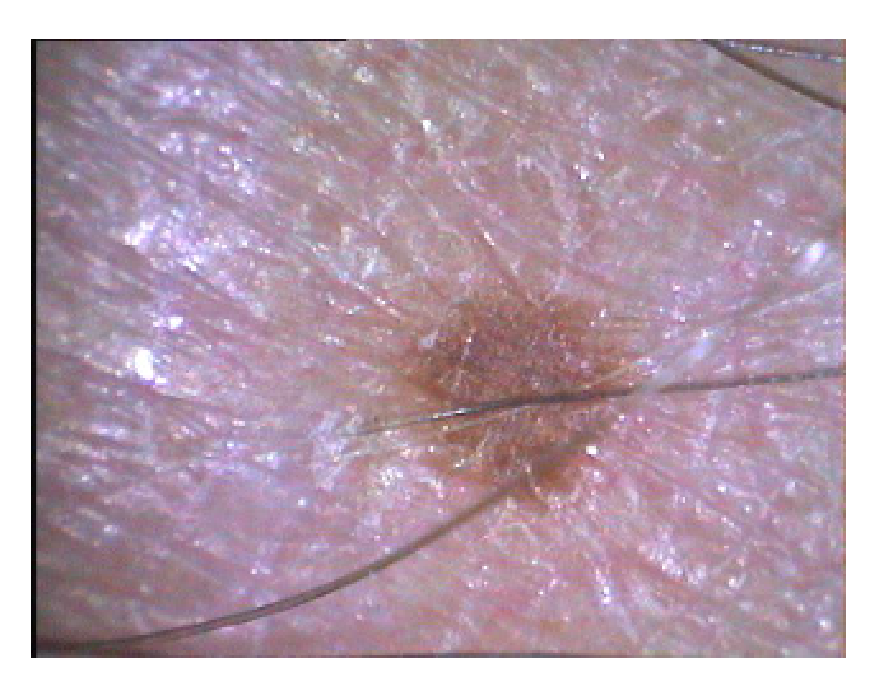
\psfig{file="./images/cpeli.eps",height=5cm,clip=}
  \hfill
  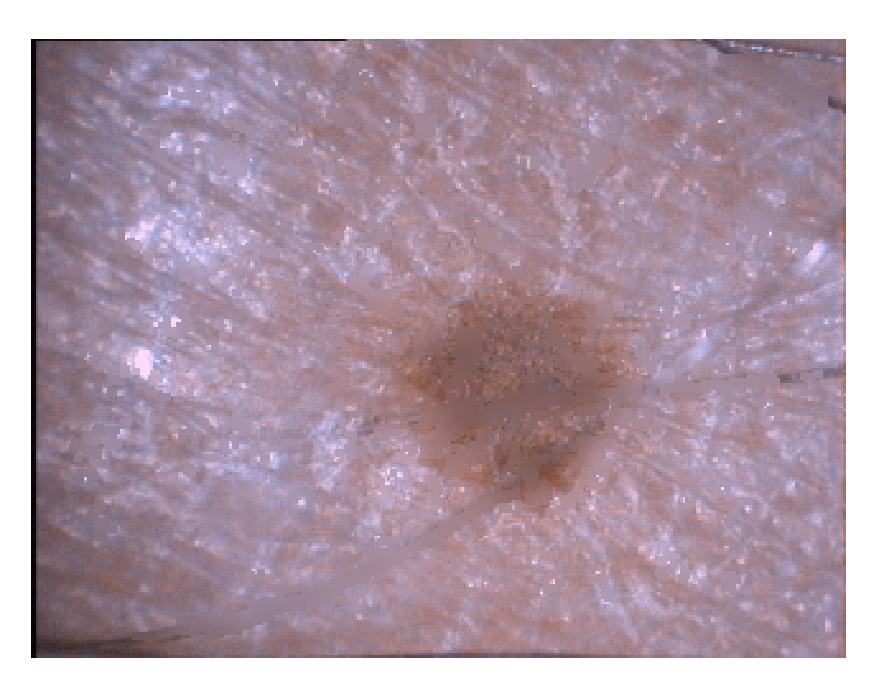
\psfig{file="./images/spelio.eps",height=5cm,clip=}}
 \centerline{
  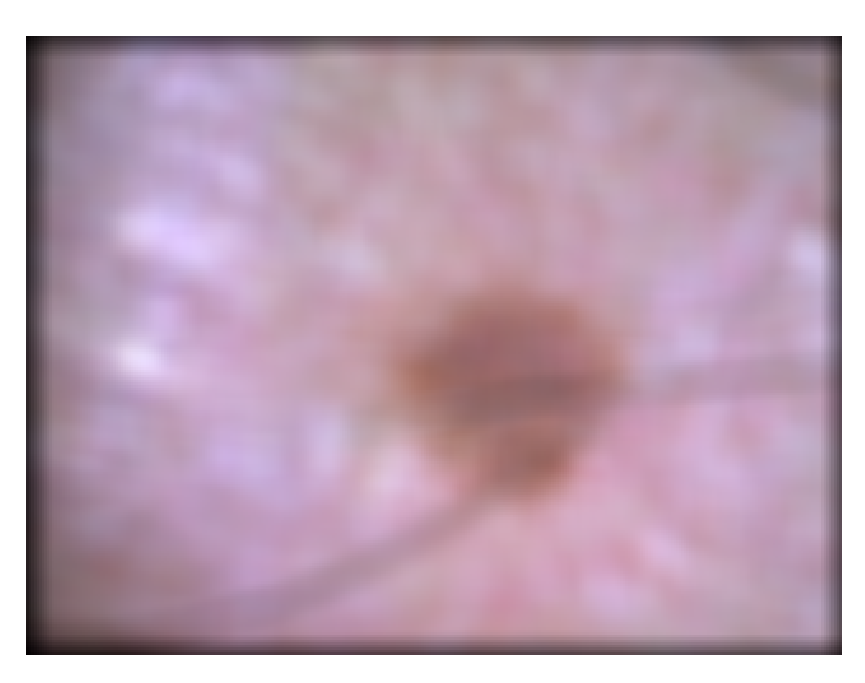
\psfig{file="./images/spelig.eps",height=5cm,clip=}
  \hfill
  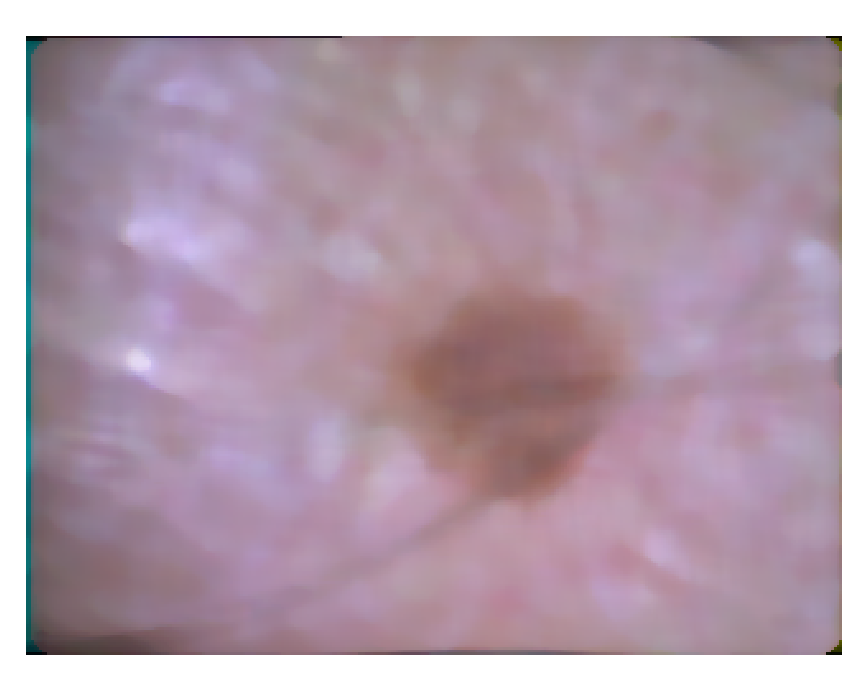
\psfig{file="./images/spelim.eps",height=5cm,clip=}}
 \caption[Attenuazione degli elementi di disturbo: peli]
  {Attenuazione degli elementi di disturbo: peli.\\
   {\sl In alto a sinistra \r{elpeli}.a}. Immagine originale.
   {\sl In alto a destra \r{elpeli}.b}. Utilizzo della
   misura di anisotropia definita dalla (\r{lam}) applicata alla componente principale della
   {\it trasformata di K.-L.} seguita da una sogliatura per individuare i punti pi\u probabilmente
   appartenenti ai peli. Quindi si \e sostituita una finestra circostante a ciascun punto con
   il valore di mediana della stessa.
   {\sl In basso a sinistra \r{elpeli}.c}. Applicazione del filtro passa-basso gaussiano.
   {\sl In basso a destra \r{elpeli}.d}. Applicazione filtro a mediana su tutta l'immagine.}
 \lb{elpeli}
\end{figure}

Si \e considerato invece di utilizzare un operatore locale, come
la stessa mediana, applicato per\o non su tutta l'immagine ma solo in corrispondenza del
disturbo individuato attraverso la misura di anisotropia definita dalla (\r{lam}).
La misura \e effettuata sulla prima componente della {\it trasformata di K.-L.} e la mappa che se
ne ottiene \e in scala di grigio con i valori massimi in corrispondenza
dei punti che appartengono a zone dell'immagine ad alta correlazione lungo una direzione.
Comunque fra i punti individuati non tutti appartengono ai peli, per cui \e necessario
introdurre un valore di soglia per selezionare quelli aventi una misura sufficientemente
elevata.

Ai punti individuati dalla sogliatura \e possibile quindi applicare un operatore locale, 
ad esempio un filtro a mediana come in Figura \r{elpeli}.

%--------------------------------------------------------------------------------------------
\subsection{Inizializzazione del contorno attivo - snake}

%.........................................................................................
\subsubsection{Motivazione}

Tenendo presente che l'immagine su cui si lavora non \e perfettamente binaria \e opportuno,
anche in relazione ai problemi di tempi di calcolo dell'evoluzione dello snake, definire
un contorno iniziale che sia il pi\u possibile prossimo a quello reale. 

Una possibilit\a \e quella di richiedere all'utente di definire alcuni punti e, ad esempio,
considerarli come i control points di una curva a B-splines e quindi costruire la curva 
che li approssima; oppure procedere ad una grossolana pre-segmentazione utilizzando
delle tecniche di binarizzazione.

Si considera in particolare quest'ultimo caso che comunque richiede un minimo apporto da parte
dell'utente che deve preselezionare sull'immagine originale un'opportuna finestra
che contenga il neo.

%.........................................................................................
\subsubsection{Processo di inizializzazione semiautomatica}

A partire dalla componente principale della {\it trasformata di K.-L.}, si effettua una riduzione 
della risoluzione applicando la (\r{campion}) ottenendo una consistente
diminuzione dei dati da analizzare e quindi del carico computazionale dei passi
successivi, sempre nell'ipotesi di approssimazione a cui si \e fatto riferimento.

Si procede quindi alla binarizzazione dell'immagine ottenuta con
i metodi indicati in (\r{segbin}).
\boss
Occorre tener presente che gli algoritmi indicati, per ragioni di efficienza, considerano
come oggetto di indagine l'istogramma del-l'immagine e non l'immagine completa,
per cui se l'area occupata dalla macchia \e circa uguale a quella circostante allora
l'istogramma normalizzato risulta abbastanza bimodale approssimando il meglio
possibile le ipotesi di validit\a su cui si basano gli algoritmi di binarizzazione.
Tale condizione pu\o essere condizionata dalla scelta dell'area da analizzare fatta
dall'utente.
\eoss

Per quanto riguarda i due metodi presentati si \e preferito quello iterativo in quanto,
fissata la tolleranza sull'approssimazione del valore di soglia in modo che non sia
eccessivamente restrittiva, si ottengono gli stessi risultati del caso dell'algoritmo di
classificazione ma in tempi inferiori.



Il risultato \e del tipo di Figura \r{neobin} in cui si pu\o notare come
non vi sia un unico elemento connesso e con contorni ben definiti, per cui si procede 
applicando in due passi successivi due operatori morfologici per ottenere una sola regione
compatta:
\ben
\im con una prima operazione di {\it apertura} si eliminano piccoli disturbi isolati e 
    l'eccessiva frastagliatura del contorno dell'elemento principale (Figura \r{neomorf}.a);
\im successivamente con un'operazione di {\it chiusura} si ottiene un unico elemento 
    compatto e, adottando un nucleo (o {\it structuring element}) circolare, con i bordi "regolari
    ({\it smooth})" (Figura \r{neomorf}.b).
\een

\begin{figure}[tbp]
 \centerline{
  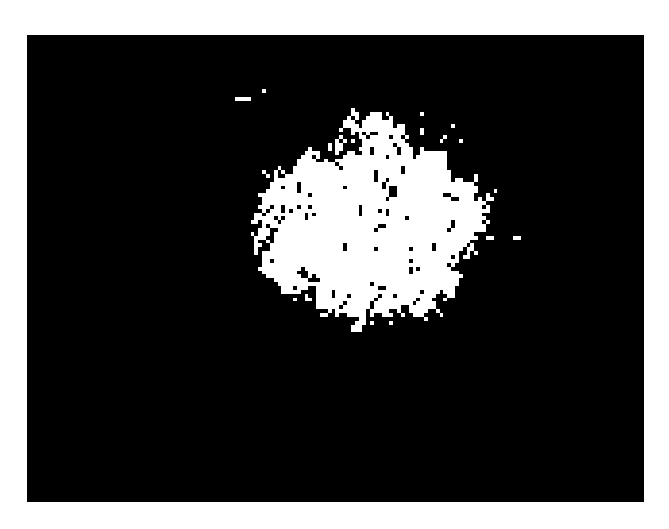
\psfig{file="./images/neobin2.eps",height=6cm,clip=}}
 \caption[Esempio di binarizzazione]
  {Esempio di binarizzazione ottenuta determinando il valore di soglia con il metodo
   iterativo proposto in (\r{segbin}). L'istogramma \e definito rispetto una regione
   definita dall'utente che circonda la macchia in modo che l'area occupata da quest'ultima
   sia prossima a quella complementare. (l'immagine riportata
   \e invece completa e non solo limitata alla finestra selezionata).}
 \lb{neobin}
 \centerline{
  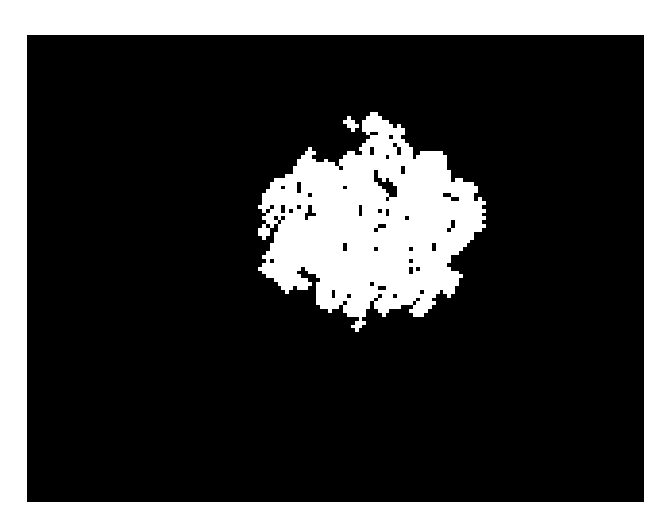
\psfig{file="./images/neobo2.eps",height=5cm,clip=}
   \hfill
  
\psfig{file="./images/neoboc2.eps",height=5cm,clip=}}
   \caption[Esempio di applicazione di operatori morfologici]
    {{\sl A sinistra \r{neomorf}.a}. Applicazione dell'operatore di apertura all'immagine binaria di
     Figura \r{neobin}: permette di eliminare i piccoli disturbi isolati e l'eccessiva 
     frastagliatura del contorno.
     {\sl A destra \r{neomorf}.b}. Applicazione dell'operatore di chiusura all'immagine di sinistra con lo
     scopo di ottenere un unico elemento compatto e con i bordi regolari; si \e perci\o
     utilizzato un nucleo (o {\it structuring element}) circolare.}
 \lb{neomorf}
\end{figure}

Il contorno attivo o {\it snake} iniziale \e ottenuto a partire dal bordo della regione appena
individuata ricorrendo ancora ad opportuni operatori morfologici:
\bdf
Sia B l'immagine binaria e K lo {\it stucturing element} scelto fra i due seguenti
$$
K\,=\,\qmatrix{1 & 1 & 1 \cr
               1 & 1 & 1 \cr
               1 & 1 & 1 \cr} \qquad o \qquad
K\,=\,\qmatrix{0 & 1 & 0 \cr
               1 & 1 & 1 \cr
               0 & 1 & 0 \cr}
$$
noti come $8-neighborhood$ e $4-neighborhood$ rispettivamente; allora l'insie-me dei punti
o pixel della matrice B che definiscono il contorno $\Gamma$ \e definito
$$
\Gamma\,=\,B\,/\,(B \ominus K)\,=\,B\,\cap\,\overline{(B \ominus K)}\,=\,
B\,\cap\,(\overline{B} \oplus K)
$$
\edf

Una volta individuato il contorno si determina la curva a {\it B-spline cubiche uniformi} che
la approssima.
Di seguito sono indicati i passi del procedimento:
\ben
\im l'insieme $\Gamma$ \e definito dai pixel $p(r,c)$, $r \in \{1,\dots,R\}$ e $c \in \{1,\dots,C\}$,
    le cui coordinate sono espresse in termini di coppie riga-colonna; per cui le si trasforma
    nel sistema di riferimento cartesiano $X-Y$;
\im i punti, nel nuovo sistema di riferiemnto, vengono ordinati in senso antiorario   
     \footnote{Oppure si parte da una descrizione del contorno in pixel gi\a definita
              in senso antiorario utilizzando ad esempio una rappresentazione tipo
              {\it chain code}.
     		  
     		  Il senso antiorario \e considerato il verso di percorrenza positivo della curva;
              risulta determinante nella relazione fra il versore tangente alla curva
              e la normale esterna.}; 
\im definendo un opportuno criterio di complessit\a \e possibile stabilire il numero di
    {\it spans} e quindi di {\it control points} (si veda il Capitolo \r{BSC}) 
    con cui descrivere una curva a B-splines che approssimi la curva di cui tali punti
    si considerano dei campioni. Per determinare i {\it control points} si procede alla
    soluzione di un sistema di equazioni lineari caratterizzato da un numero di incognite
    (i {\it control points}) inferiore ai valori noti (i punti campioni della curva)
    risolvendo un problema ai minimi quadrati;
\im considerando che la curva \e ottenuta dall'immagine originale ad una risoluzione ridotta
    occorre effettuare un cambiamento di scala opposto per riportarla
    nell'immagine originale tenendo presente che va aggiornata la componente di traslazione
    della trasformazione che lega i due sistemi di riferimento adottati: quello immagine
    e quello della curva.
\een

La definizione del criterio di complessit\a e il problema della determinazione dei 
{\it control points} sar\a esposto nei paragrafi successivi.

%===========================================================================================
\section{Algoritmo: Fase 2}

La seconda fase \e caratterizzata dall'evoluzione del contorno definito nella fase
precedente fino a raggiungere una condizione di equilibrio. Si considera come modello dello
snake la curva a B-splines cubiche uniformi la cui legge di evoluzione nel tempo \e definita
dall'algoritmo di {\it Yezzi, Tsai e Willsky} trattato in (\r{AYTW}).
\`E proposto inoltre un criterio per misurare la complessit\a del contorno della regione
da segmentare per ridefinire il numero e la distribuzione dei {\it control points}.

\balg
{\bf Evoluzione dello snake.}\par
\ben
\im \lb{PAYezzi1} A partire dal vettore dei control points ${\bf Q}$ e fissato il numero di campioni $N(i)$
    per lo span $i-esimo$, con $i=1,\dots,N_s$ con $N_s$ numero di spans della curva chiusa
    pari al numero di punti di controlllo, si pu\o calcolare il vettore ${\bf X}$ dei 
    campioni della curva. 
    Successivamente si calcolano i versori tangenti ${\bf X}_s$ e normali ${\bf X}_n$ alla
    curva nei punti ${\bf X}$ e la curvatura $k$ della curva in ${\bf X}$.
\im Calcolo di aree e medie interne ed esterne e dalla (\r{EYezzi}) lo stato energetico
    dello snake.
\im Se si \e raggiunta la condizione di minima energia, rispetto alle condizioni fissate,
    allora il processo di segmentazione \e concluso, altrimenti si continua con
    l'aggiornamento della curva.
\im Con il passo di aggiornamento si determina il nuovo vettore di punti ${\bf Y}$
    ottenuto da ${\bf X}$ secondo la legge di evoluzione definita dalla discretizzazione della
    (\r{flow}).
\im Ogni $T$ passi \e possibile aumentare il numero dei punti di controllo $N_s$ e 
    ridistribuire i campioni ${\bf Y}$ della curva secondo il criterio di complessit\a fissato. 
\im A partire da ${\bf Y}$ e $N_s$ (o eventualmente i loro aggiornamenti) si determina il nuovo
    vettore ${\bf Q}$ dei punti di controllo che definisce la curva a B-splines che meglio
    approssima, ai minimi quadrati, la curva i cui campioni sono dati da ${\bf Y}$.
\im Si ritorna al passo \r{PAYezzi1}.
\een
\ealg

Vediamo ora in dettaglio i singoli passi.

%--------------------------------------------------------------------------------------------
\subsection{Passo 1: calcolo di ${\bf X}$, ${\bf X}_s$, ${\bf X}_n$, $k$}

\`E possibile esprimere tali vettori in funzione dei punti di controllo definendo opportune
matrici ${\bf A}$, ${\bf A}_s$ e ${\bf A}_{ss}$ (si veda l'Appendice \r{A2}).\par
Considerata la curva chiusa $\Gamma$ descritta per mezzo delle B-splines cubiche e 
uniformi dalla carta ${\bf r}(s,t)$ e discretizzandola rispetto alla variabile $s$ \e possibile
ottenere il vettore dei campioni
\be
{\bf X}\,=\,{\bf A}\,{\bf Q}
\ee
I versori ${\bf \tau}$ tangenti alla curva sono definiti, nel continuo, dalla
\be
{\bf \tau}({\bf r}(s,t))\,=\,\frac{{\bf r}_s(s,t)}{\|{\bf r}_s(s,t)\|}
\ee
che applicata ai punti di ${\bf X}(i)$, $i=1,\dots,N_p$ risulta
\be
{\bf \tau}({\bf X}(i))\,=\,\frac{{\bf X}_s(i)}{\|{\bf X}_s(i)\|} \quad con \quad {\bf X}_s\,=\,{\bf A}_s\,{\bf Q}.
\ee
Considerato che ${\bf \tau}$ definisce l'orientamento positivo di percorrenza della curva,
che qui \e considerato antiorario, \e possibile calcolare la normale esterna ${\bf n}$ non
appena si fissi l'orientamento positivo del piano che \e considerato dal versore ${\bf e}_3$;
per cui risulta
\be
{\bf n}({\bf r}(s,t))\,=\,{\bf \tau}\wedge{\bf e}_3({\bf r})\,=\,(\tau_y,-\tau_x,0)
\ee
e che si riduce alla coppia $(\tau_y,-\tau_x)$; quindi esprimibile dalla 
\be
{\bf n}({\bf r}(s,t))\,=\,\smatrix{2}{ 0 & 1 \cr
                                      -1 & 0 \cr}{\bf \tau}
\ee
Riferito ai campioni della curva vale
\be
{\bf X}_n(i)\,=\,\smatrix{2}{ 0 & 1 \cr
                       -1 & 0 \cr}{\bf \tau}(X(i)).
\ee

Per quanto riguarda la curvatura si considera la definizione
\be
k({\bf r}(s,t))\,=\,\frac{{\bf r}_s(s,t) \wedge {\bf r}_{ss}(s,t)}{\|{\bf r}_s(s,t)\|^3}
\ee
che rappresenta la curvatura con segno della curva ${\bf r}(s,t)$; che si semplifica nella
\be
k({\bf X}(i))\,=\,\frac{{\bf X}_s(i) \wedge {\bf X}_{ss}(i)}{\|{\bf X}_s(i)\|^3}
\ee
dove ${\bf X}_{ss}={\bf A}_{ss}\,{\bf Q}$.
\`E possibile definire anche il vettore curvatura diretto lungo la normale esterna
${\bf k}\,=\,k\,{\bf n}$.

%--------------------------------------------------------------------------------------------
\subsection{Passo 2: calcolo delle medie e aree interne ed esterne alla curva}

La funzione energia definita da Yezzi et al. \cite{Yezzi} e la relativa legge di aggiornamento
prevedono il calcolo del vettore delle medie e delle aree delle regioni interna ed esterna
rispetto alla curva chiusa.

Considerando che dalla Fase 1 si ottiene una curva iniziale che \e abbastanza
prossima al contorno finale \e conveniente applicare la versione locale suggerita nello stesso
articolo: ovvero la regione interna compresa fra la curva $\Gamma$ e la curva interna
$\Gamma^{int}$ e la regione esterna fra $\Gamma$ e $\Gamma^{est}$.

Le due nuove curve possono essere ottenute sfruttando quanto visto a proposito dell'invarianza
delle curve a B-splines nei confronti delle omotetie (Figura \r{omotetia}).

Sfruttando la versione locale si evita di dover considerare la zona vicine
ai bordi dell'immagine maggiormente soggetta ai disturbi dovuti agli effetti di bordo
dell'ottica del sensore e ad una illuminazione non uniforme.

%--------------------------------------------------------------------------------------------
\subsection{Passo 3: la condizione di equilibrio}

L'evoluzione dello snake termina quando la funzione energia ha raggiunto il punto di minimo
ovvero, come punto di estremo, ha gradiente nullo.
Fra le due condizioni, teoricamente equivalenti, si \e scelta la prima in quanto pi\u
semplice da determinare una volta note le due medie; la seconda infatti richiede di 
verificare che l'incremento fra due istanti successivi \e trascurabile per ogni campione della
curva.

In condizioni ideali la funzione ${\cal E}(t)$, che descrive l'andamento dell'energia durante
l'evoluzione dello snake, \e monotona decrescente fino alla condizione di equilibrio, e
poi rimane costante, per cui il minimo \e individuato nel momento in cui vale
${\cal E}(t^\ast)={\cal E}(t^\ast +1)$ per i due istanti successivi $t^\ast$ e $t^\ast +1$.

Nelle condizioni reali invece ci\o non vale a causa delle approssimazioni introdotte e quindi
per stabilire il raggiungimento della condizione di equilibrio \e pi\u opportuno valutare
l'andamento dell'energia negli ultimi $T_e$ passi di calcolo; in particolare si considera
la funzione
\be
\epsilon(t)\,=\,\frac{1}{|{\cal E}(t)|}\,
                \frac{1}{T_e}\,\sum_{t-T_e+1}^{t}\,|{\cal E}(t)-{\cal E}(t-1)|
\ee

che rappresenta la media dei valori assoluti delle variazioni dell'energia totale degli
ultimi $T_e$ passi di calcolo relativa all'energia all'istante $t$.

Si considera ${\cal E}(t)$ "costante" quando $\epsilon(t)$ \e inferiore ad un valore
prefissato che essendo espresso in termini relativi \e indipendente dal valore di
${\cal E}(t)$.

%--------------------------------------------------------------------------------------------
\subsection{Passo 4: aggiornamento della curva in base alla legge di evoluzione}

Come detto si considera il modello di {\it snake} la cui legge di evoluzione \e data dalla (\r{flow})
\be
\frac{d \Gamma}{dt}\,=\,\sum_{j=1}^{N}\,(m_j^{int}-m_j^{est})\,
              \bigg[\frac{P_j-m_j^{int}}{A^{int}}\,+\,\frac{P_j-m_j^{est}}{A^{est}}\bigg].
\ee
Per poterla applicare \e necessario discretizzarla sia nella variabile spaziale sia in 
quella temporale; per quanto riguarda la prima si procede come sopra considerando i campioni
della curva dati da ${\bf r}_i$, mentre per la variabile temporale si approssima la
derivata con il rapporto incrementale (un'approssimazione del primo ordine):
\be
\frac{d \Gamma}{dt}\,=\,\frac{\Gamma (t + \Delta t)-\Gamma (t)}{\Delta t}
\ee
da cui si ottiene 
\be
\Gamma (t + \Delta t)\,=\,\Gamma (t)\,+\,\frac{d \Gamma}{dt}\,\Delta t
\ee
ovvero
\be
{\bf Y}(i)\,=\,{\bf X}(i,t + 1)\,=\,{\bf X}(i,t)\,+\,g(k_i)\frac{d \Gamma}{dt}\,({\bf X}(i))
\ee

\boss
Le coordinate dei campioni ${\bf X}$ sono definite in $[0,C]\times[0,R]\subset\M(R)^2$, mentre
le primitive $P_j$ sono definite per i pixels di coordinate $(r,c)$ appartenenti a
$\{1,R\}\times\{1,C\}\subset\M(N)^2$, con $R$ e $C$ numero di righe e di colonne, quindi \e
necessario poter stabilire l'intensit\a della primitiva da associare al campione della
curva.
Il punto $X(i)=(x_i,y_i)$ pu\o essere associato al pixel di riga $r=\lceil y_i \rceil$
e colonna $c=\lceil x_i \rceil$( \footnotemark ), per cui l'intensit\a della primitiva \e
$P(r,c)$.
\footnotetext{Si fa riferimento al caso in cui il sistema di riferimento cartesiano della
curva ha l'origine coincidente con lo spigolo in alto a sinistra della matrice $P$ e con
gli assi $X$ e $Y$ diretti lungo le colonne e le righe rispettivamente.}

Per tener conto che il punto non \e necessariamente al centro del pixel e del fatto che il
valore del pixel stesso potrebbe essere affetto da rumore \e opportuno considerare $P$ su una
finestra di pixel nell'intorno di quello fissato; ad esempio considerando la media pesata
o la mediana dei valori dei pixel della finestra.
\eoss

%.......................................................................................
\subsubsection{La funzione guadagno g(k)}

Si noti che l'"incremento temporale" $\Delta t$ \e stato conglobato nella
funzione $g(k)$ che definisce un opportuno guadagno che dipende dalla curvatura nel
punto $i-esimo$ $X(i)$.
La dipendenza del guadagno dalla curvatura permette di modulare l'incremento in funzione 
delle caratteristiche locali della curva riducendo il peso delle misure effettuate in
tratti ad elevata curvatura che potrebbero determinare la formazione di cappi.

Tenendo presente che $k$ \e la curvatura con segno, la funzione guadagno deve essere pari,
per cui una possibile scelta \e data dalla gaussiana
\be
g(k)\,=\,g_0\,\exp(- \alpha k^2)
\ee
dove $g_0$ \e il guadagno massimo e il fattore $\alpha$ definisce la forma del filtro.

La scelta di $g_0$ va fatta tenendo conto che se da un lato pu\o aumentare la velocità
dello {\it snake}, ovvero ridurre i tempi di convergenza, dall'altro pu\o renderlo instabile
o fare in modo che l'evoluzione si arresti su minimi relativi non corrispondenti al bordo
dell'oggetto che si vorrebbe identificare. 

%.......................................................................................
\subsubsection{Gli insiemi di livello}

Nell'articolo \cite{Yezzi} gli autori utilizzano gli {\it insiemi di livello} ({\it level set}) \cite{Malladi}
come soluzione per l'implementazione della legge di evoluzione; tale metodo permette inoltre
di realizzare in modo efficiente e automatico le operazioni topologiche di divisione e fusione
di {\it snakes} per poter individuare pi\u oggetti presenti nell'immagine a partire da una sola
curva oppure da pi\u curve ({\it semi}) disseminate sull'immagine.

La possibilit\a di realizzare tali trasformazioni non \e 
presente negli altri modelli di snake se non con l'aggiunta di procedure supplementari 
(come nel caso proposto in \cite{Terzopoulos}). 

Nel nostro caso comunque si \e scelto di adottare la legge espressa nella sua forma originale
e procedere a semplici discretizzazioni.

%--------------------------------------------------------------------------------------------
\subsection{Passo 5: il criterio di complessit\a della curva}

Nella fase di inizializzazione dello {\it snake} vengono individuati un certo numero di control
points che si ritiene sufficiente a descrivere il contorno dell'oggetto individuato dalla
binarizzazione, numero che potrebbe non essere comunque sufficiente in relazione alla
complessit\a effettiva dell'elemento da segmentare.

Durante l'evoluzione inoltre si pu\o trovare che un certo numero di campioni \e maggiormente
concentrato in un tratto della curva non eccessivamente complesso, e con essi anche un
maggior numero di control points, con conseguenze negative per la regolarit\a della curva
stessa (si veda \r{PSCBS}).
Si \e deciso perci\o di ricostruire una nuova sequenza di campioni da ridistribuire ad un
nuovo insieme di punti di controllo di dimensioni diverse dal precedente; in questo modo
si scorrela l'evoluzione della curva dai passi precedenti accelerando la convergenza al
risultato finale.

%.......................................................................................
\subsubsection{Ricampionamento della curva}

Dato il vettore di punti ${\bf Y}$ ottenuto nel passo precedente, si considera la poligonale
i cui vertici sono proprio gli elementi di ${\bf Y}$ e a questa si sovrappone un particolare
reticolo e si determinano le intersezioni ${\bf \Upsilon}(i)$ fra la poligonale e il reticolo:
quest'ultime costituiscono i nuovi campioni della curva (Figura \r{reticolo}).

\begin{figure}[tbp]
 \centerline{
  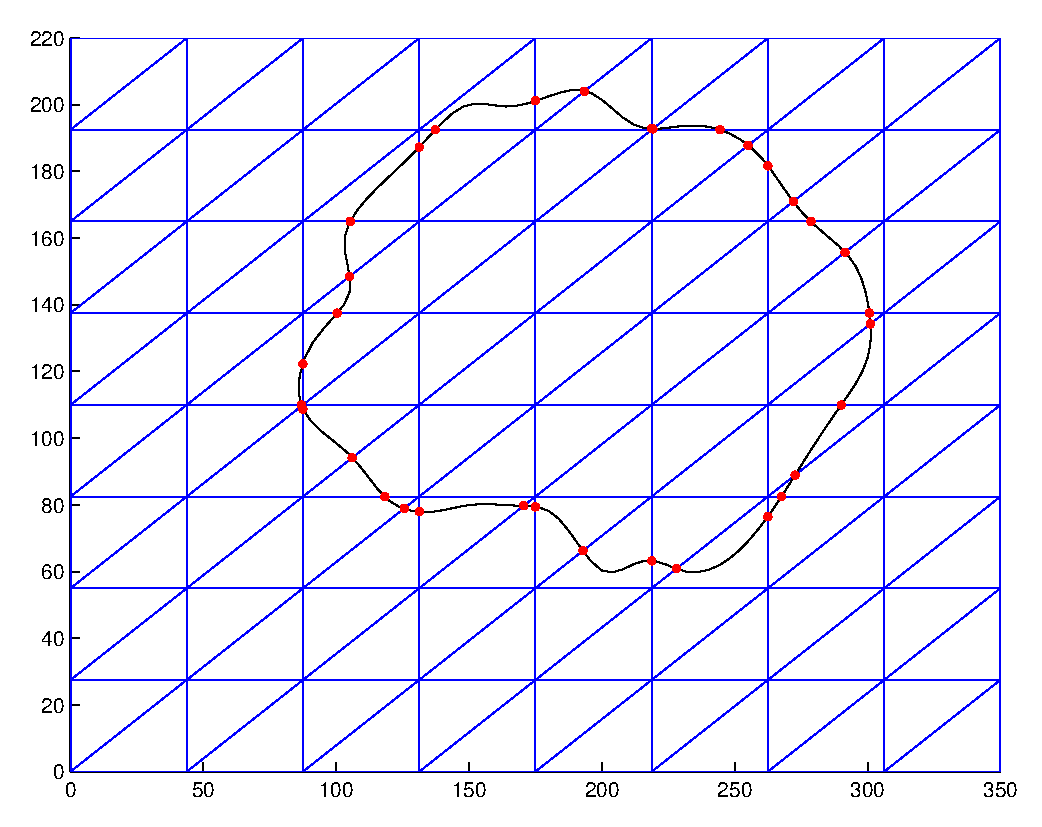
\psfig{file="./images/reticolo.eps",height=6cm,clip=}}
 \caption[Riparametrizzazione dello snake a B-splines]
  {Ricampionamento dello {\it snake} a B-splines realizzato intersecando la curva con un 
   reticolo ottenuto come scomposizione simpliciale, a simplessi triangolari, del piano
   immagine. I nuovi campioni ${\bf \Upsilon}(i)$ corrispondono alle intersezioni.}
 \lb{reticolo}
\end{figure}

Il reticolo introdotto rappresenta un esempio di {\it reticolazione simpliciale} o 
{\it triangolazione} del piano che risulta scomposto nella somma di {\it simplessi} topologici,
che nel caso in esame sono i singoli triangoli \footnotemark, che offre i seguenti vantaggi:

\footnotetext{La scomposizione simpliciale \e sviluppata nell'ambito della Topologia
Algebrica.}

\bi 
\im una rappresentazione univoca della curva;
\im variando la densit\a del reticolo \e possibile controllare il grado di 
approssimazione del contorno e di conseguenza anche
la velocit\a di convergenza al risultato finale.
\ei

Si osserva che la scelta della riparametrizzazione con l'uso della triangolazione simpliciale
\e utilizzata in \cite{Terzopoulos} per implementare le trasformazioni topologiche.
 
%.......................................................................................
\subsubsection{Definizione del criterio di complessit\a}

I nuovi campioni vengono successivamente distribuiti ai nuovi spans in modo che la 
complessit\a di ciascun span sia entro un limite massimo prefissato ${\cal M}$ interpretabile
come la "massa" totale dello span.

\bdf
{\bf Complessit\a.}\par
Per ciascun punto ${\bf \Upsilon}(i)$ si considerano i due vettori ${\bf u}(i)$ e ${\bf v}(i)$
$$
{\bf u}(i)=\frac{{\bf \Upsilon}(i-1)-{\bf \Upsilon}(i)}{L} \qquad
{\bf v}(i)=\frac{{\bf \Upsilon}(i+1)-{\bf \Upsilon}(i)}{L},
$$
normalizzati rispetto la lunghezza $L$ della poligonale di vertici ${\bf \Upsilon}(i)$, e le due
funzioni 
$$
d(i)\,=\,d({\bf u}(i),{\bf v}(i))\,=\,\|{\bf u}(i)\|+\|{\bf v}(i)\|
$$
$$
c(i)\,=\,c({\bf u}(i),{\bf v}(i))\,=\,\|{\bf u}(i)+{\bf v}(i)\|
$$
che descrivono i due contributi della complessit\a della "curva" nel punto: il primo tiene
conto della distanza fra i due vertici precedente e successivo, in senso antiorario, mentre
il secondo del grado di allineamento fra i tre punti (una sorta di curvatura).
Entrambi sono normalizzati rispetto alla lunghezza (perimetro) della poligonale in modo
da rendere il procedimento indipendente dalle dimensioni.

La complessit\a totale \e definita dalla combinazione dei due termini secondo i pesi $w_d$ e
$w_c$:
\be
\mu(i)\,=\,w_d\,d(i)\,+\,w_c\,c(i)
\ee
\edf

\boss
Nell'applicazione considerata, si sono ottenuti migliori risultati con $w_d > w_c$.
\eoss

Quindi nota la "densit\a" $\mu(i)$ si suddivide il vettore $\Upsilon$ in {\it spans} aventi
"massa" minore o al pi\u uguale a ${\cal M}$; in tal modo si determina la nuova
lunghezza del vettore dei control points $N_s^{\,\prime}$ per i quali vanno aggiornate le
matrici ${\bf A}$, ${\bf A}_s$ e ${\bf A}_{ss}$ che saranno utilizzate all'inizio del successivo
passo di evoluzione dello snake.

\begin{figure}[tbp]
 \centerline{
  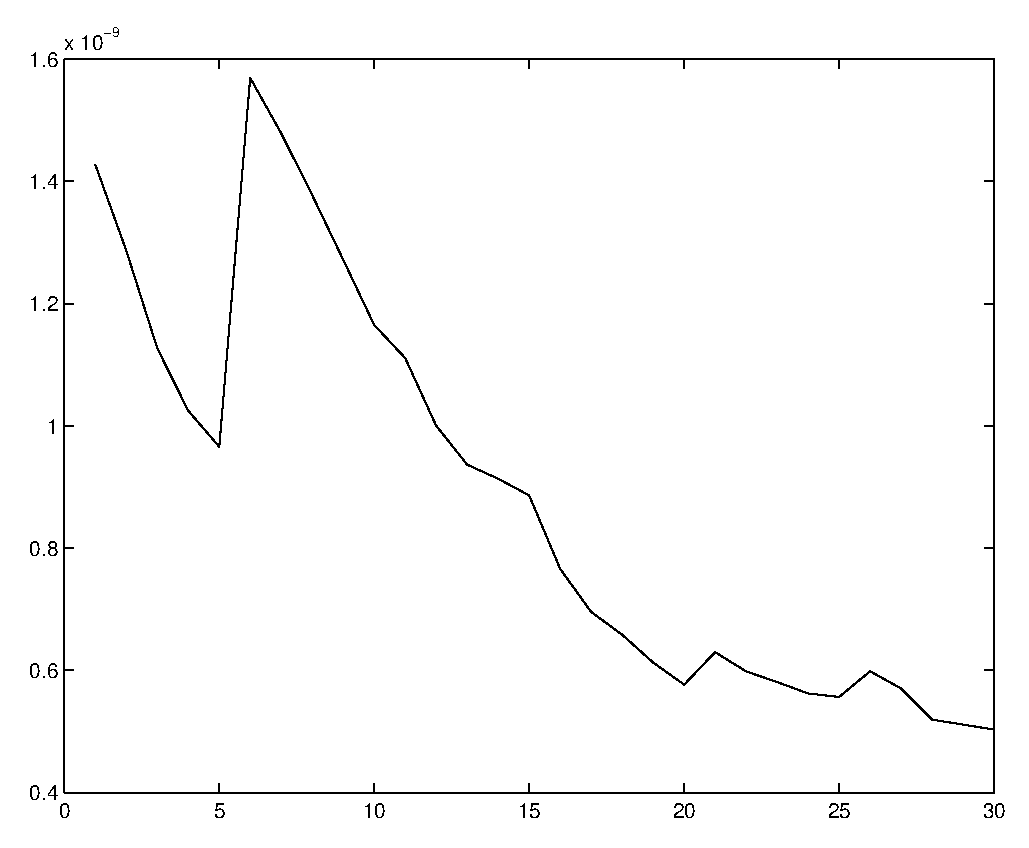
\psfig{file="./images/Ec.eps",height=5cm,clip=}
   \hfill
  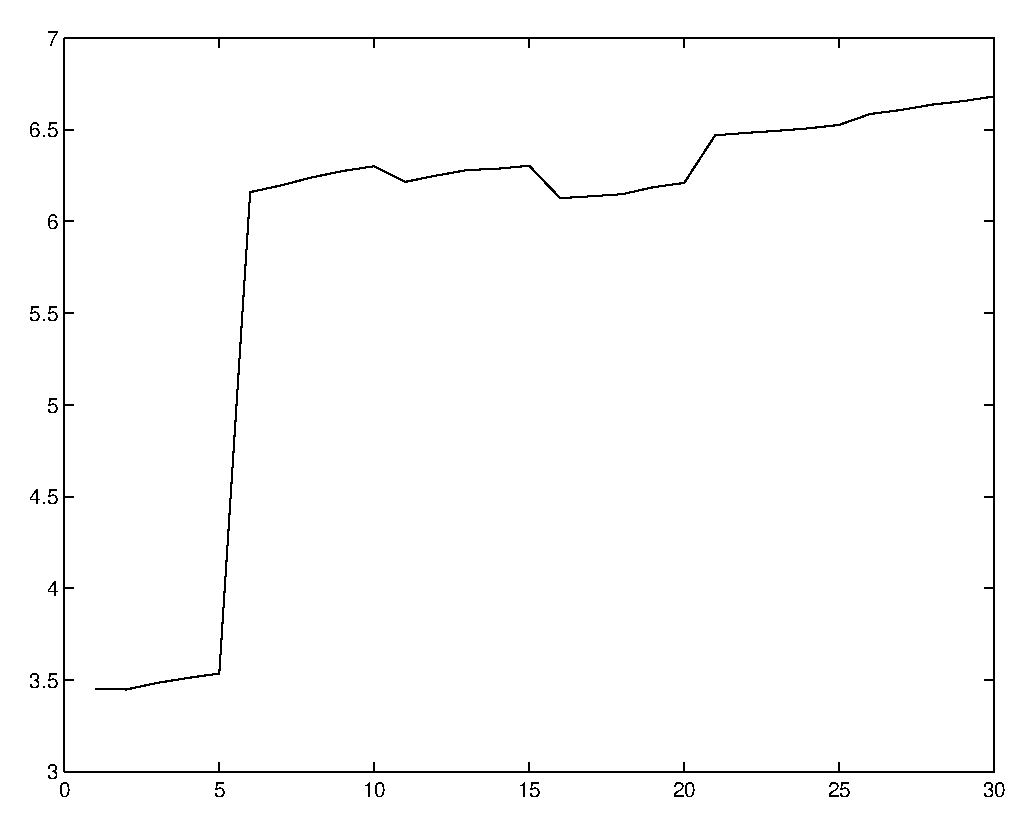
\psfig{file="./images/Et.eps",height=5cm,clip=}}
   \caption[Energie dello snake]
    {{\sl A sinistra \r{energie}.a}. Energia delle "forze" deformanti (si veda il testo).
     {\sl A destra \r{energie}.b}. Modulo dell'energia totale dello snake (\r{EYezzi}).}
 \lb{energie}
\end{figure}

In Figura \r{energie}.a mostra è rappresentato l'andamento dell'energia dei
campioni della funzione $(d \Gamma / dt)({\bf X}(i))$, ovvero la norma $L_2$ dello stesso vettore,
che si pu\o pensare indicativa delle "forze" deformanti che agiscono sullo {\it snake};
la \r{energie}.b mostra invece il modulo dell'energia dello snake valutata secondo la
(\r{EYezzi}).

Man mano che si procede verso lo stato di equilibrio finale si ha mediamente una diminuzione
della prima in quanto si \e sempre pi\u vicini all'o-biettivo finale (come se agisse una forza
elastica) mentre la seconda aumenta, ovvero l'energia con segno del sistema diminuisce,
coerentemente con le ipotesi fatte sullo stato di equilibrio a minima energia potenziale.

%--------------------------------------------------------------------------------------------
\subsection{Passo 6: la rappresentazione a B-splines della curva aggiornata}

Ad ogni ciclo sia che si abbia una ridistribuzione dei punti ${\bf \Upsilon}$ sia che si
considerino direttamente i punti ottenuti dal processo di aggiornamento $\bf Y$, si procede
alla determinazione della rappresentazione della curva a {\it B-splines 
cubiche uniformi} che approssima i campioni ottenuti calcolando il nuovo vettore di control points $\hat{\bf Q}$.

A partire dall'espressione definita precedentemente ${\bf X}={\bf A}\,{\bf Q}$, che lega i
control points ai campioni della curva, \e possibile ricavare una soluzione al problema
inverso ovvero ottenere i control points dai campioni ${\bf \Upsilon}$.

Per il sistema di equazioni lineari
\be
{\bf A}\,{\bf Q}\,=\,{\bf \Upsilon},
\ee
dove il numero di vincoli (equazioni) \e superiore al numero di incognite (${\bf Q}$), 
si considera il problema in termini di approssimazione ai minimi quadrati,
ovvero si considera come soluzione il vettore $\hat{\bf Q}$ per cui \e minima la norma 
$\|\,{\bf \Upsilon}\,-\,{\bf A}\,\hat{\bf Q}\|$.

La soluzione \e unica ed \e data da
\be
\hat{\bf Q}\,=\,{\bf A}^{\dagger}\,{\bf \Upsilon} 
\ee
dove ${\bf A}^{\dagger}=({\bf A}^{T}{\bf A})^{-1}){\bf A}^{T}$ \e la
{\it pseudo-inversa sinistra} di ${\bf A}$.
 
%===========================================================================================
\section{Risultati}

Nelle Figure \r{risIm}, \r{risIsa} e \r{risIp} sono visualizzati alcuni esempi di risultati
dell'ap-plicazione dell'algoritmo di segmentazione sviluppato.

Dalle Figure \r{risIm} e \r{risIsa} si pu\o notare che l'algoritmo \e abbastanza insensibile
alla condizione iniziale fissata per il contorno attivo, in funzione comunque della qualit\a
dell'immagine elaborata: nel primo caso infatti vi sono dei disturbi dovuti a fenomeni di
riflessione in prossimit\a dei bordi.
Nel secondo caso invece le due soluzioni sono abbastanza simili, la differenza tra le due
inizializzazioni \e soprattutto in relazione al tempo di calcolo necessario per raggiungere 
l'equilibrio finale.

In Figura \r{risIp} \e evidenziato il problema della presenza dei peli in prossimit\a dei
bordi e il miglioramento del risultato se si fa precedere una fase di preelaborazione con
un operatore locale anisotropo basato sulla misura di anisotropia definita dalla (\r{lam}).

\finepar

\begin{figure}[tbp]
 \centerline{
  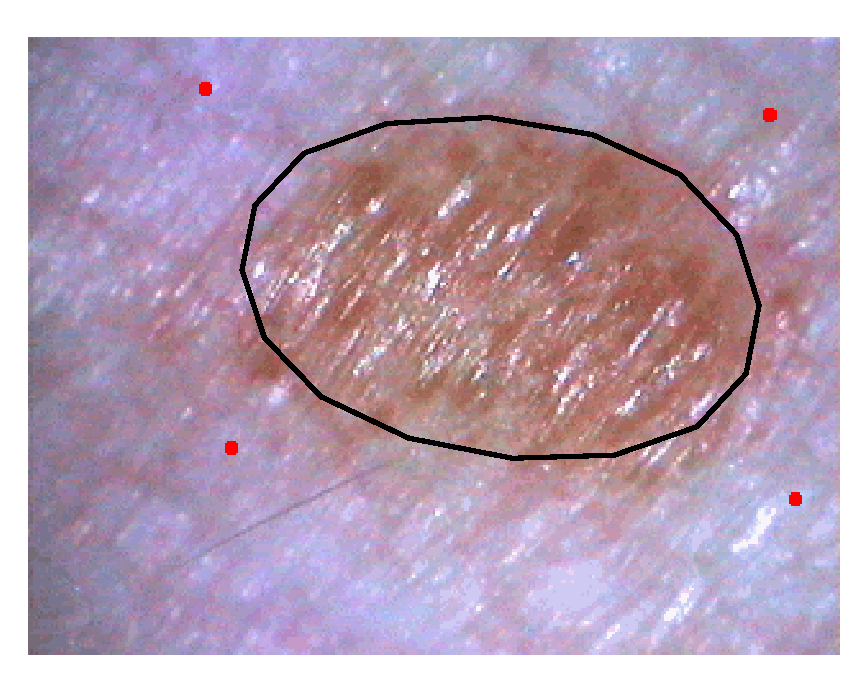
\psfig{file="./images/ris1I1o.eps",height=5cm,clip=}
   \hfill
  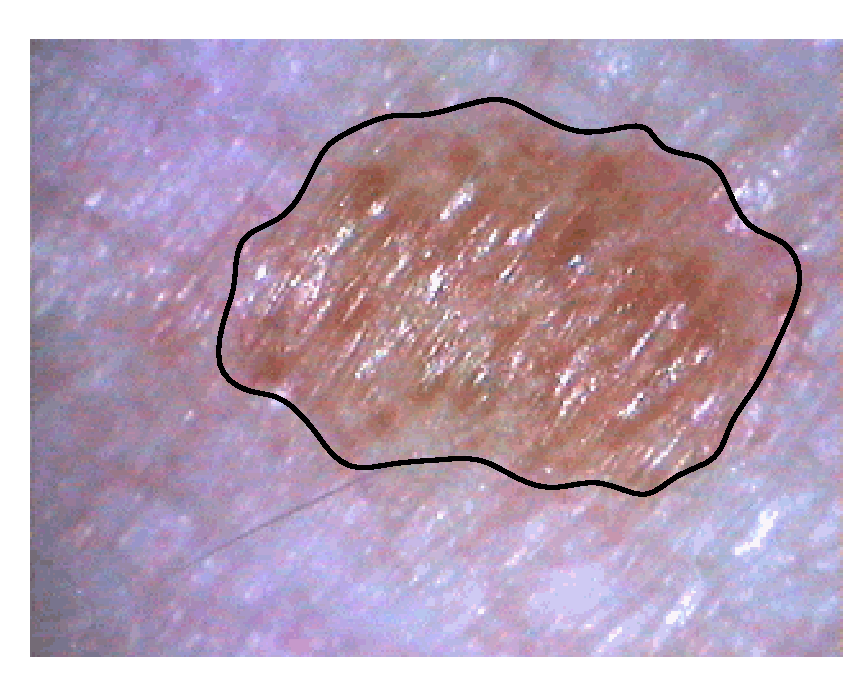
\psfig{file="./images/ris1I1.eps",height=5cm,clip=}}
 \centerline{
  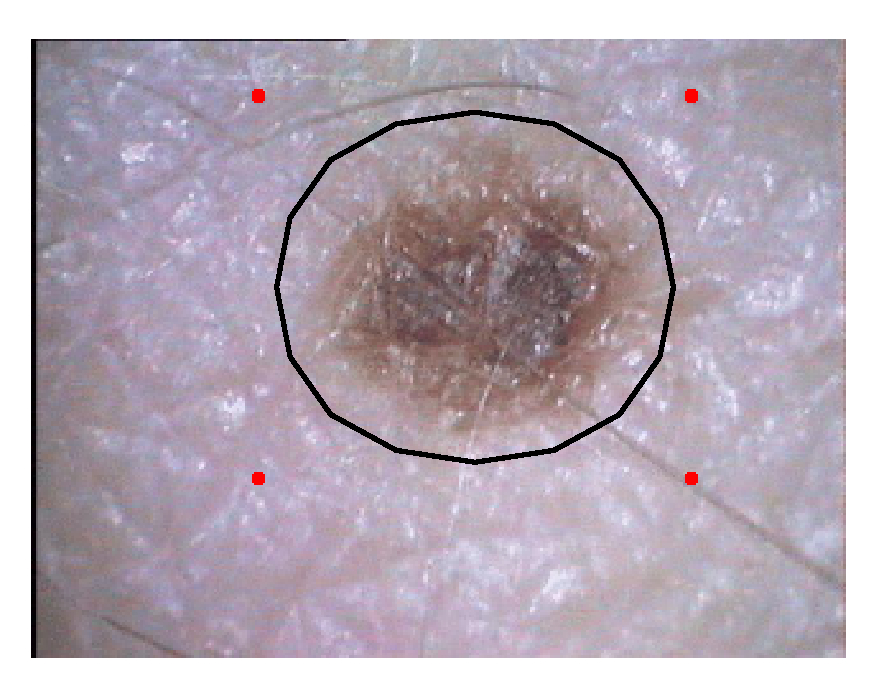
\psfig{file="./images/rI2o.eps",height=5cm,clip=}
   \hfill
  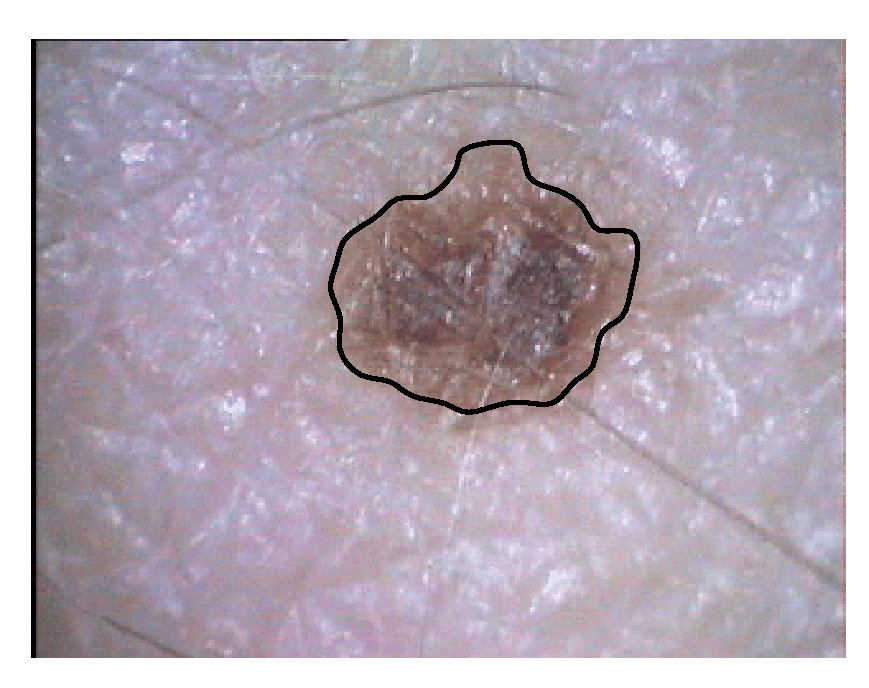
\psfig{file="./images/rI2f.eps",height=5cm,clip=}}
   \caption[Risultato della segmentazione con inizializzazione manuale]
    {{\sl A sinistra}: inizializzazione manuale del contorno iniziale; sono evidenziati i $4$
     punti di controllo e la curva a B-splines che li approssima. {\sl A destra}: risultato 
     della segmentazione.}
 \lb{risIm}
\end{figure}

\begin{figure}[tbp]
 \centerline{
  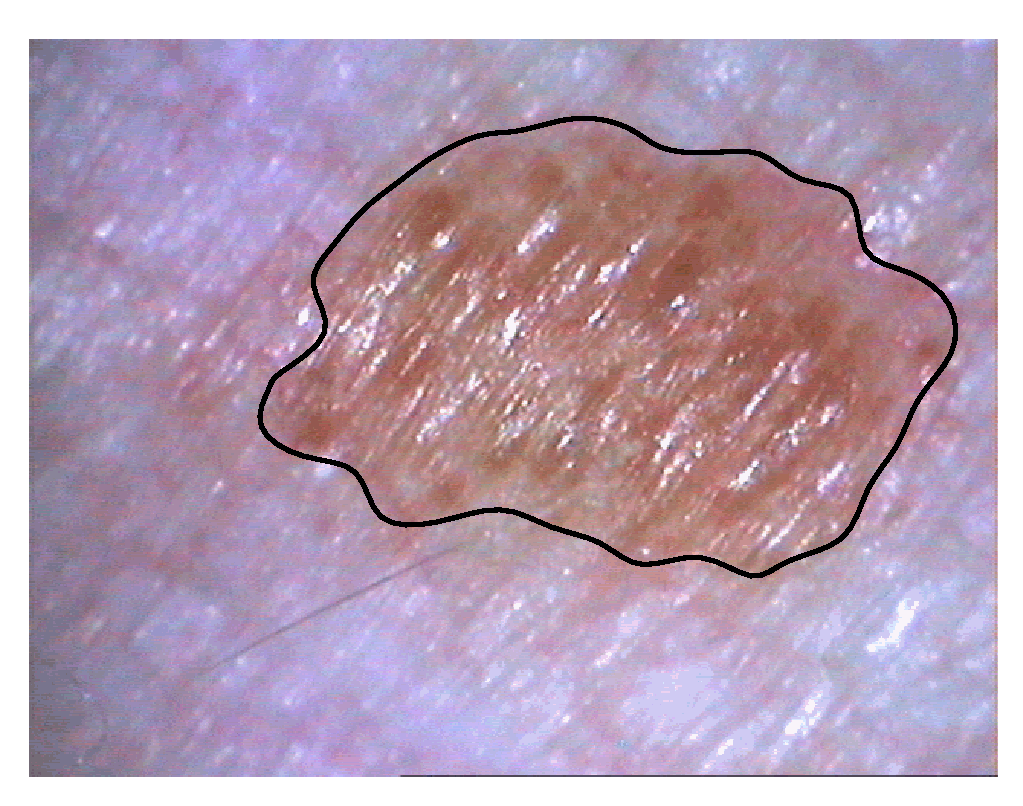
\psfig{file="./images/segfin1.eps",height=5cm,clip=}
   \hfill
  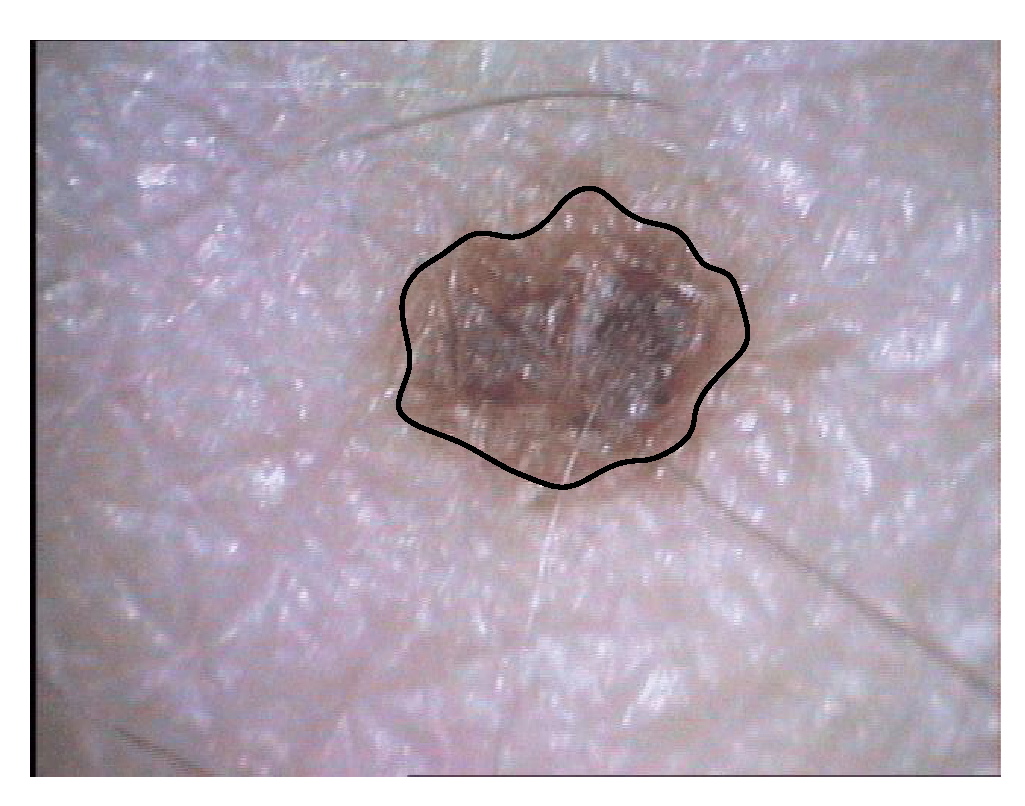
\psfig{file="./images/segfin2.eps",height=5cm,clip=}}
   \caption[Risultato della segmentazione con inizializzazione semiautomatica]
    {Due risultati dell'applicazione dell'algoritmo di segmentazione con inizializzazione
     semiautomatica, dove il contorno iniziale \e ricavato dal bordo della regione compatta
     ottenuta dalla binarizzazione della componenete principale della trasformata di K.L.
     dell'immagine originale.}
 \lb{risIsa}
\end{figure}

\begin{figure}[tbp]
 \centerline{
  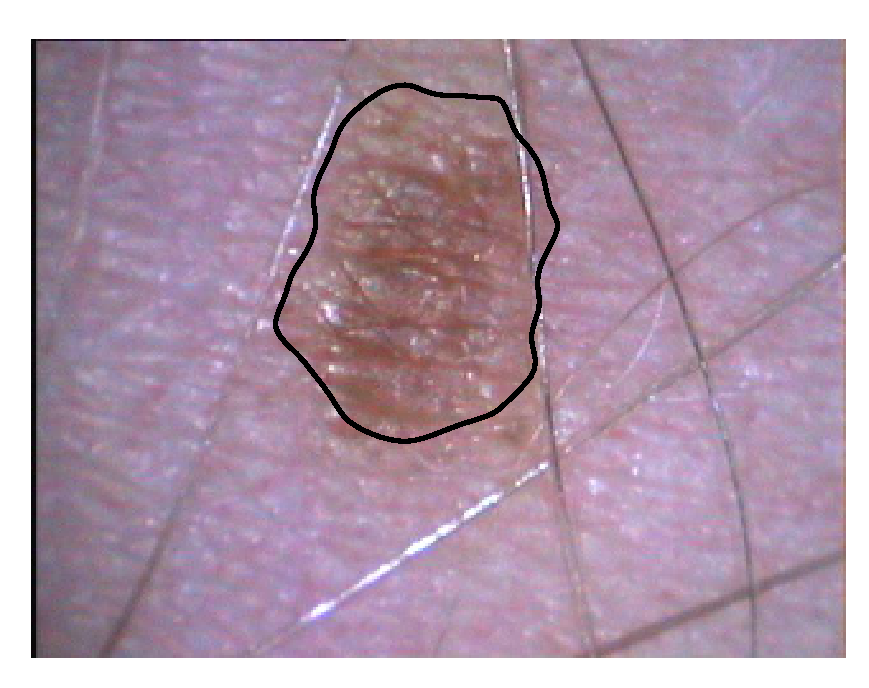
\psfig{file="./images/r3I9.eps",height=5cm,clip=}
   \hfill
  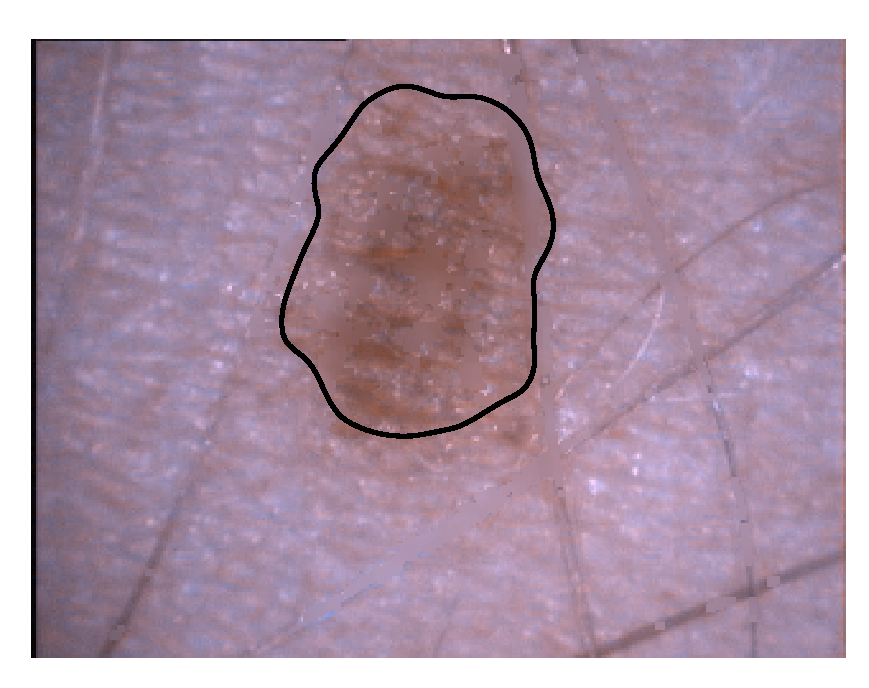
\psfig{file="./images/r2I9.eps",height=5cm,clip=}}
   \caption[Risultato della segmentazione con l'applicazione di un operatore anisotropo per la
    riduzione dei disturbi]
    {{\sl A sinistra}: applicazione dell'algoritmo di segmentazione direttamente all'immagine
     originale. {\sl A destra}: il processo di segmentazione \e preceduto da una fase di 
     preelaborazione in cui si riduce l'effetto di disturbo dei peli con l'applicazione
     di un operatore locale anisotropo.}
 \lb{risIp}
\end{figure}

 



% Conclusioni
\chapter{Conclusioni}

In questa tesi \e proposto un algoritmo si segmentazione per l'individuazione dei contorni
di macchie cutanee il cui nucleo \e costituito dal metodo di segmentazione basato su un
interessante modello di contorno attivo o {\it snake} proposto da Yezzi et al. in \cite{Yezzi}.
Esso infatti combina i vantaggi dei due approcci con cui vengono affrontati i problemi di
segmentazione: quello basato sulla propriet\a di omogeneit\a dei segmenti e quello che
realizza la segmentazione individuando i bordi che separano i segmenti.

Per ottenere inoltre una rappresentazione compatta dello stesso contorno, in vista delle
successive misure, si \e scelta la sua rappresentazione a B-splines cubiche uniformi.
Visto per\o che la forma dell'oggetto da segmentare non \e nota a priori vi \e la necessit\a
di definire un metodo per permettere allo snake di adattarsi alla diversa complessit\a
della macchia da individuare.
Si \e perci\o considerato un metodo che sfrutta la riparametrizzazione della curva a partire
dai campioni ottenuti dall'intersezione con un reticolo, che \e la scomposizione simpliciale 
(o triangolazione) del piano immagine, e la successiva ripartizione di tali punti fra
i nuovi {\it control points}, in funzione di un criterio di complessit\a che tiene conto della
distanza e del grado di allineamento, o "curvatura", fra i campioni.

Dai test effettuati si \e visto che l'algoritmo \e poco sensibile
all'inizia-lizzazione del contorno attivo, comunque per ridurre i tempi di calcolo \e opportuno
che la curva iniziale sia prossima al bordo dell'oggetto da segmentare.
Per questo si \e
definita una procedura di inizializzazione basata sul contorno della regione compatta ottenuta
dalla binarizzazione, e successiva elaborazione morfologica, della componente principale della
{\it trasformata di Karhunen-Lo\`eve} dell'immagine originale.

In relazione ai tempi di esecuzione si pu\o dire che il punto critico \e dato dal calcolo delle
medie interne ed esterne alla curva, \e quindi opportuno considerare con attenzione una 
possibile approssimazione della funzione intensit\a delle primitive.

\`E stato definito inoltre un operatore locale basato su una particolare misura di anisotropia
per ridurre l'effetto di disturbo dei peli, non sempre 
trascurabile nel momento in cui tali elementi si trovano in prossimit\a del bordo e quindi
possono influenzare la dinamica dello {\it snake}.

L'algoritmo \e stato sviluppato per la segmentazione di macchie cutanee, ma come \e
strutturato e per la natura del modello di snake \e potenzialmente applicabile ad altri
oggetti non appena siano caratterizzabili con un opportuno vettore di primitive ({\it features}).

\finepar

%===================================================================================

\begin{appendici}

\appendice{Matrici per B-splines cubiche uniformi}\lb{A}

%===========================================================================================
\section{Matrice di omotetia}\lb{A1}

Dato il vettore dei {\it control points} ${\bf X}=[{\bf x}_i]$ che descrivono la curva,  
e il centroide ${\bf c}$ \e definito da
\be
{\bf c}\,=\,\frac{1}{m}\,\sum_{i=0}^{m-1}\,{\bf x}_i.
\ee
si considerino ${\bf z}_i={\bf x}_i-{\bf c}$ i raggi vettore uscenti da ${\bf c}$ verso gli ${\bf x}_i$.

Applicando l'omotetia di fattore $\gamma$ i nuovi raggi vettore $\hat{\bf z}_i$ risultano
\be
\hat{\bf z}_i\,=\,\gamma\,{\bf z}_i
\ee
per cui i nuovi control points si ottengono da
\beqa
\hat{\bf x}_i & = & \hat{\bf z}_i\,+\,{\bf c}\, 
                    \,=\,\gamma\,({\bf x}_i-{\bf c})\,+\,{\bf c}\,= \nonumber\\
              & = & \gamma\,{\bf x}_i\,+\,(1-\gamma)\,{\bf c}\, 
                    \,=\,\gamma\,{\bf x}_i\,+\,\frac{1-\gamma}{m}\,{\bf 1}_{1 \times m}\,{\bf X}
\eeqa
Quindi il nuovo vettore di {\it control points} risulta 
\beqa
\hat{\bf X} & = & \gamma\,\qmatrix{     1 &     0 & \dots  &      0 \cr
                                        0 &     1 & \dots  &      0 \cr
                                   \vdots & \dots & \ddots & \vdots \cr
                                        0 & \dots & \dots  &      1 \cr}\,{\bf X}\,+\,
                  \frac{1-\gamma}{m}\qmatrix{     1 &     1   \dots  &      1 \cr
                                                  1 &     1 & \dots  &      1 \cr
                                             \vdots & \dots & \ddots & \vdots \cr
                                                  1 & \dots & \dots  &      1 \cr}\,{\bf X}
                  \nonumber\\
            &   & \nonumber\\
            & = & \Big[\,\gamma\,{\bf I}_m\,+\,\frac{1-\gamma}{m}\,{\bf 1}_m\,\Big]\,{\bf X}\,=\,
                  {\bf R}(\gamma)\,{\bf X}
\eeqa
con ${\bf I}_m$ matrice identica di ordine $m$ e ${\bf 1}_m$ matrice $m \times m$ di "$1$".
 
Esprimendo la rappresentazione a B-spline della curva nella forma
\be
{\bf r}(u)\,=\,\sum_{i=0}^{m-1}\,B_i(u)\,{\bf x}_i\,=\,{\bf B}(u)\,{\bf X}                                                      
\ee
dove ${\bf B}(u)$ e ${\bf X}$ sono rispettivamente i vettori delle basi $B_i$ e dei control
points, la curva trasformata risulta
\be
\hat{\bf r}(u)\,=\,{\bf B}(u)\,{\bf R}(\gamma)\,{\bf X}.                                                     
\ee

%===========================================================================================
\section{Matrici per la rappresentate a B-splines di curve}\lb{A2}

A partire dalla (\r{cBsmat}), \e possibile rappresentare in termini di prodotto di matrici 
la carta a B-splines che descrive lo span $i-esimo$, $i=0,\dots,N_s-1$, della curva
$\Gamma$
\be
{\bf r}_i(s)\,=\,\frac{1}{6}\,{\bf s}^T\,{\bf M}\,{\bf Q}_i
\ee
dove ${\bf s}=[s^3,s^2,s,1]^T$, $s\in[0,1]$, $M$ \e la matrice $(4 \times 4)$ che descrive
la forma della B-spline $B$ di riferimento, e ${\bf Q}_i$ \e la quaterna di {\it control
points} che definiscono come si combinano i quattro tratti di cubica (Capitolo \r{BSC}).

Si proceda quindi alla discretizzazione di $s$ a cui corrispondono i campioni ${\bf r}_i(s_j)$
per $s_j=j/N_c$ con $j=0,\dots,N_c-1$ e $N_c$ il numero di campioni per span; si ottiene 
quindi, per il singolo campione, 
$$
X_i(j)\,=\,\frac{1}{6}\,{\bf s}_j^T\,{\bf M}\,{\bf Q}_i
$$
e incolonnando per tutti i campioni dello span 
\be
{\bf X}_i\,=\,\hat{\bf A}_i\,{\bf Q}_i
\ee 
$$
\hat{\bf A}_i=\frac{1}{6}\,\qmatrix{{\bf s}_0^T \cr
                                         \vdots \cr 
                                    {\bf s}_j^T \cr
                                         \vdots \cr
                                    {\bf s}_{N_c-1}^T \cr}\,{\bf M}\,=\,
              {\bf S}_i\,{\bf M} \qquad (N_c \times 4)
$$

Un'ulteriore passo nella semplificazione dell'espressione \e fatto considerando 
${\bf Q}_i={\bf G}_i{\bf Q}$, con ${\bf Q}$ vettore completo dei control points;
quindi riassumendo si ottiene
\be
{\bf X}\,=\,\qmatrix{      {\bf X}_0 \cr
                              \vdots \cr 
                           {\bf X}_i \cr
                              \vdots \cr
                     {\bf X}_{N_s-1} \cr}\,=\,
\qmatrix{            \hat{\bf A}_0\,{\bf G}_0 \cr
                                       \vdots \cr 
                     \hat{\bf A}_i\,{\bf G}_i \cr
                                       \vdots \cr
         \hat{\bf A}_{N_s-1}\,{\bf G}_{N_s-1} \cr}\,=\,{\bf A}\,{\bf Q}
\ee
con ${\bf X}\,(N_s\,N_c \times 2)$, ${\bf A}\,(N_s\,N_c \times N_s)$ e ${\bf Q}\,(N_s \times 2)$.

Le matrici ${\bf G}_i\,(4 \times N_s)$ legano lo span $i-esimo$ con i relativi {\it control points}
in ${\bf Q}$. 
Si noti che rispetto a quanto detto nel Capitolo \r{BSC} \e possibile rappresentare un circuito senza aggiungere
i primi tre {\it control points} alla fine del vettore ma direttamente attraverso la matrice ${\bf A}$.

\vs(5)

Per chiarire la struttura delle ${\bf G}_i$ si considera l'esempio in cui $N_s=5$:
$$
{\bf G}_0\,=\,\qmatrix{ 1 & 0 & 0 & 0 & 0 \cr
                        0 & 1 & 0 & 0 & 0 \cr
                        0 & 0 & 1 & 0 & 0 \cr
                        0 & 0 & 0 & 1 & 0 \cr}, \quad
{\bf G}_1\,=\,\qmatrix{ 0 & 1 & 0 & 0 & 0 \cr
                        0 & 0 & 1 & 0 & 0 \cr
                        0 & 0 & 0 & 1 & 0 \cr
                        0 & 0 & 0 & 0 & 1 \cr}, \quad \dots
$$
Come si pu\o notare la seconda matrice \e ottenuta traslando verso destra la diagonale di $1$,
ovvero moltiplicando la matrice ${\bf G}_0$ per una matrice ${\bf K}$ quadrata $(N_s \times N_s)$
$$
{\bf K}\,=\,\qmatrix{ 0 & 1 & 0 & 0 & 0 \cr
                      0 & 0 & 1 & 0 & 0 \cr
                      0 & 0 & 0 & 1 & 0 \cr
                      0 & 0 & 0 & 0 & 1 \cr
                      1 & 0 & 0 & 0 & 0 \cr}
$$
Il risultato pu\o essere esteso anche alle altre matrici ${\bf G}_i$ per cui vale
$$
{\bf G}_{i+1}\,=\,{\bf G}_i\,{\bf K} \qquad i=0,\dots,N_s-2 
$$
e dove ${\bf G}_0$ ha una struttura nota
$$
{\bf G}_0\,=\,\qmatrix{{\bf I}_4 & | &{\bf O}_{4,N_s-4} \cr}.
$$ 
 
\vs(5)

Per ottenere le matrici ${\bf A}_s$ e ${\bf A}_{ss}$ \e sufficiente considerare che derivando
rispetto a $s$ la ${\bf r}_i(s)$ si ottiene 
\be
{\bf r}_{i_s}(s)\,=\,\frac{1}{6}\,{\bf s}_s^T\,{\bf M}\,{\bf Q}_i
\ee
con ${\bf s}_s=[3s^3,2s,1,0]$; per cui \e sufficiente modificare le singole ${\bf S}_i$.

Analogamente per la derivata seconda rispetto $s$.

\finepar 
 
    




\appendice[Funzionali definiti su regioni regolari]
          {Gradiente di funzioni integrali definite su regioni regolari}\lb{B}

%========================================================================================
%\section{}

\blem
Data ${\bf A}$, matrice quadrata $(n \times n)$, ${\bf x}$ e ${\bf y}$ due vettori colonna
$n-dim$ allora vale
 \be
 {\bf A}\,{\bf x}\cdot{\bf y}\,-\,{\bf A}\,{\bf y}\cdot{\bf x}\,=\,
             {\bf x}\cdot\Big[{\bf A}^T-{\bf A}\Big]\,{\bf y}.
 \ee
\lb{lemmaB1}
\elem

\begin{proof}
  Dalla definizione di prodotto scalare $(\cdot)$  
 $$
 {\bf A}\,{\bf x}\cdot{\bf y}\,=\,({\bf A}\,{\bf x})^T\,{\bf y}
 $$
 e dalla commutativit\a si ha che 
 $$
 {\bf A}\,{\bf x}\cdot{\bf y}\,-\,{\bf A}\,{\bf y}\cdot{\bf x}\,=\,
 {\bf x}^T\,{\bf A}^T\,{\bf y}\,-\,{\bf x}^T\,{\bf A}\,{\bf y}\,=\,
 $$
 $$ 
 {\bf x}^T\,\Big[{\bf A}^T-{\bf A}\Big]\,{\bf y}\,=\,
 {\bf x}\cdot\Big[{\bf A}^T-{\bf A}\Big]\,{\bf y}. 
 $$
\end{proof}


Sia
\be 
h(t)\,=\,\ds\int_{R(t)}\,f(x,y)\,dxdy
\ee
con $R(t)$ la regione racchiusa dalla curva chiusa $\Gamma(t)$ e $f:\M(R)^2 \longrightarrow \M(R)$
una funzione continua.

Definita la funzione vettoriale {\bf g}(x,y) con
\be
g_1(x,y)\,=\,-\,\ds\int_0^y\,f(x,\lambda)\,d\lambda \qquad
g_2(x,y)\,=\,\ds\int_0^x\,f(\lambda,y)\,d\lambda
\ee
\e possibile scrivere
\be
h(t)\,=\,\ds\int_{R(t)}\,\frac{1}{2}\,
 \Bigg[\frac{\partial g_2}{\partial x}\,(x,y)\,-\,\frac{\partial g_1}{\partial y}\,(x,y)\Bigg]
 \,dxdy
\ee

Dal {\it teorema di Stokes}, che nel caso in esame di curve piane si riduce alle {\it formule
di Green}, si ottiene 
\be 
h(t)\,=\,\frac{1}{2}\ds\int_{\Gamma(t)}\,{\bf g}\cdot{\bf \tau}\,dl.
\ee
Considerando che $\Gamma(t)$ \e rappresentata dalla carta ${\bf r}(s,t)=[x(s,t),y(s,t)]$,
con $s \in [0,1]$\footnotemark, e che il vettore tangente alla curva \e esprimibile in funzione
della parametrizzazione
\be
{\bf \tau}(s,t)\,=\,\frac{{\bf r}_s(s,t)}{\|{\bf r}(s,t)\|}
\lb{tau}
\ee
risulta
\be
h(t)\,=\,\frac{1}{2}\ds\int_0^1\,{\bf g}\cdot\frac{{\bf r}_s(s,t)}{\|{\bf r}(s,t)\|}\,
         {\|{\bf r}(s,t)\|}\,ds\,=\,
       \,\frac{1}{2}\ds\int_0^1\,{\bf g}\cdot{\bf r}_s(s,t)
\ee

\footnotetext{Si \e scelto il dominio del parametro $s$ in $[0,1]$ per comodit\aac; \e
comunque valido un qualsiasi intervallo del tipo $[\omega_o,\omega_1]$.} 

Calcolare $\nabla h$ lungo la curva regolare $\Gamma$ \e equivalente a massimizzare la
variazione $h^{\,\prime}(t)$
\be
h^{\,\prime}(t)\,=\,\frac{1}{2}\ds\int_0^1\,\Bigg[{\bf g}_t\cdot{\bf r}_s(s,t)\,+\,
                                            {\bf g}\cdot{\bf r}_{s,t}(s,t)\Bigg]\,ds.
\ee

Integrando per parti rispetto a $s$ il secondo termine dell'integranda risulta
\beqa
\ds\int_0^1\,{\bf g}\cdot{\bf r}_{s,t}(s,t)
  & = & {\bf g}\cdot{\bf r}_t\Big\vert_{s=0}^{s=1}\,
        -\,\ds\int_0^1\,{\bf g}_s\cdot{\bf r}_t(s,t)\,ds\,= \nonumber\\
  & = & -\,\ds\int_0^1\,{\bf g}_s\cdot{\bf r}_t(s,t)\,ds 
\eeqa
in quanto il primo addendo \e nullo dato che la curva \e chiusa e quindi 
${\bf r}(0)={\bf r}(1)$ per cui ${\bf g}({\bf r}(0))={\bf g}({\bf r}(1))$ e cos\iac\,pure 
${\bf r}_t(0)={\bf r}_t(1)$.

Considerando inoltre che il differenziale di funzioni composte
\beqa
{\bf g}_s & = & {\bf g}_s({\bf r}(s,t))\,=\,J{\bf g}(x,y){\bf r}_s(s,t) \nonumber \\
          &   & \\
{\bf g}_t & = & {\bf g}_t({\bf r}(s,t))\,=\,J{\bf g}(x,y){\bf r}_t(s,t), \nonumber
\eeqa
con
$$
J{\bf g}(x,y)\,=\,
\smatrix{2}{{\ds\frac{\partial g_1}{\partial x}} & {\ds\frac{\partial g_1}{\partial y}} \cr
        {\ds\frac{\partial g_2}{\partial x}} & {\ds\frac{\partial g_2}{\partial y}}}(x,y)\,=\,
\smatrix{2}{ 0 & -f \cr
             f &  0 }(x,y)\,=\,
$$
\be
=\,f(x,y)\,\smatrix{2}{ 0 & -1 \cr
                        1 &  0 },
\lb{jac}
\ee
assieme alle precedenti si ottiene l'espressione per $h^{\,\prime}(t)$
\be
h^{\,\prime}(t)\,=\,\frac{1}{2}\ds\int_0^1\,\Big[J{\bf g}\,{\bf r}_t\cdot{\bf r}_s\,-\,
                    J{\bf g}\,{\bf r}_s\cdot{\bf r}_t\Big]\,ds.
\ee

Applicando il Lemma \r{lemmaB1} con ${\bf x}={\bf r}_t$, ${\bf A}=J{\bf g}$ e
${\bf y}={\bf r}_s$ 
\be
h^{\,\prime}(t)\,=\,\frac{1}{2}\ds\int_0^1\,
                  \Big[{\bf r}_t\cdot\bigg((J{\bf g})^T-J{\bf g}\bigg)\,{\bf r}_s\Big]\,ds
\lb{hprime}
\ee

Dalla (\r{jac}) si vede che lo {\it Jacobiano} \e antisimmetrico, per cui lo \e pure la
differenza $(J{\bf g})^T-J{\bf g}$ che infatti vale
$$
2\,f(x,y)\,\smatrix{2}{  0 & 1 \cr
                        -1 & 0 },
$$
dato che per la propriet\a di antisimmetria $(J{\bf g})^T=-J{\bf g}$.

Sostituendo nella (\r{hprime}) 
\be
h^{\,\prime}(t)\,=
         \,\ds\int_0^1\,\Big[{\bf r}_t\cdot\,f\,\smatrix{2}{  0 & 1 \cr
                                                             -1 & 0 }\,{\bf r}_s\Big]\,ds
\lb{hprime2}
\ee

Nell'ipotesi per cui l'orientamento positivo di percorrenza di $\Gamma$ sia quello antiorario
e che l'orientamento positivo della regione $R$ sia ${\bf e}_3$ allora sussiste la relazione
fra il versore tangente e quello normale alla curva 
$$
{\bf n}\,=\,\smatrix{2}{  0 & 1 \cr
                         -1 & 0 }\,{\bf \tau};
$$
considerando inoltre l'espressione (\r{tau}) si ha
\be
\|{\bf r}_s\|\,{\bf n}\,=\,\smatrix{2}{  0 & 1 \cr
                                        -1 & 0 }\,{\bf r}_s.
\ee 

Quest'ultimo \e uno dei termini del prodotto scalare dell'integranda in (\r{hprime2}) e 
quindi
\be
h^{\,\prime}(t)\,=
         \,\ds\int_0^1\,\Big[{\bf r}_t\cdot\,f\,{\bf n}\Big]\,\|{\bf r}_s\|\,ds\,=\,
         \,\ds\int_{\Gamma(t)}\,{\bf r}_t\cdot\,f\,{\bf n}\,dl
\lb{hprime3}
\ee
per cui la direzione lungo la quale deformare la curva $\Gamma$ in modo che sia massima
$h^{\,\prime}$ \e data dal flusso 
$$
{\bf r}_t\,=\,f\,{\bf n}.
$$


\finepar

\end{appendici}

%=================================
% Bibliografia

\bibliographystyle{plain}

\bibliography{tesibib}

%=================================
\end{document}
